%% Käytä toinen näistä:
%% ensimmäinen, jos käytät pdflatexia, joka kääntää tekstin suoraan 
%% pdf-tiedostoksi (kuvat on oltava jpg- tai pdf-tiedostoina)
%% toinen, jos haluat tuottaa ps-tiedostoa (käytä eps-formaattia kuville,
%% alä käytä ps-muotoisia kuvia!)


%% Käytä näitä, jos kirjoitat englanniksi. Katso englanninokset tiedostosta
%% thesistemplate.tex.
\documentclass[english,12pt,a4paper,pdftex,elec,utf8]{aaltothesis}
%\documentclass[english,12pt,a4paper,dvips]{aaltothesis}

\usepackage{graphicx}
\usepackage[binary-units=true]{siunitx}
%\sisetup{detect-family}
%\AtBeginDocument{\sisetup{math-rm=\mathrm, text-rm=\rmfamily}}

%% Matematiikan fontteja, symboleja ja muotoiluja lisää, näitä tarvitaan usein 
\usepackage{amsfonts,amssymb,amsbsy}

\usepackage{listings}
\usepackage[super]{nth}
\usepackage{csquotes}
\usepackage{tikz}
\usetikzlibrary{shapes,arrows}
\usetikzlibrary{dsp, chains}
\usetikzlibrary{arrows, decorations.markings}
\DeclareMathAlphabet{\mathpzc}{OT1}{pzc}{m}{it}
\newcommand{\z}{\mathpzc{z}}
\usepackage{pgfplots}
\usepackage{amsmath,bm,times}
\newcommand{\mx}[1]{\mathbf{\bm{#1}}} % Matrix command
\newcommand{\vc}[1]{\mathbf{\bm{#1}}} % Vector command

\renewcommand{\labelenumii}{\theenumii}
\renewcommand{\theenumii}{\theenumi.\arabic{enumii}.}

\newcommand{\Clanguage}{\lstset{
  language=C++,                % choose the language of the code
  basicstyle=\ttfamily,
  %numbers=left,                   % where to put the line-numbers
  %stepnumber=1,                   % the step between two line-numbers.        
  %numbersep=5pt,                  % how far the line-numbers are from the code
  %backgroundcolor=\color{white},  % choose the background color. You must add \usepackage{color}
  %showspaces=false,               % show spaces adding particular underscores
  %showstringspaces=false,         % underline spaces within strings
  %showtabs=false,                 % show tabs within strings adding particular underscores
 % tabsize=2,                      % sets default tabsize to 2 spaces
 % captionpos=b,                   % sets the caption-position to bottom
  %breaklines=true,                % sets automatic line breaking
  %breakatwhitespace=true,         % sets if automatic breaks should only happen at whitespace
  title=\lstname,                 % show the filename of files included with \lstinputlisting;
}}

%% Jos et jostain syystä pidä, miten alla oleva hyperref-paketti käyttää
%% fontteja, värejä yms., käytä tämän paketin makroja muuttamaan
%% fonttimäärittelyt. Katso paketin dokumentaatiota. Paketti määrittelee
%% \url-makron, joten ota paketti käyttöön, jos et käytä hyperref-pakettia.
%%
%\usepackage{url}

%% Saat pdf-tiedoston viittaukset ja linkit kuntoon seuraavalla paketilla.
%% Paketti toimii erityisen hyvin pdflatexin kanssa. 
%%
\usepackage{hyperref}
\hypersetup{pdfpagemode=UseNone, pdfstartview=FitH,
  colorlinks=true,urlcolor=red,linkcolor=blue,citecolor=black,
  pdftitle={Default Title, Modify},pdfauthor={Your Name},
  pdfkeywords={Modify keywords}}

%\usepackage{textcomp}

\usepackage[backend=biber,
style = numeric]{biblatex}
\addbibresource{bibliography.bib}
%% Kaikki mikä paperille tulostuu, on tämän jälkeen
\begin{document}

%% Korjaa vastaamaan korkeakouluasi, jos automaattisesti asetettu nimi on 
%% virheellinen 
%%
%% Change the school field to specify your school if the automatically 
%% set name is wrong
% \university{aalto-yliopisto}
% \school{Sähkötekniikan korkeakoulu}

%% Vain kandityölle: Korjaa seuraavat vastaamaan koulutusohjelmaasi
%%
\degreeprogram{Elektroniikka ja sähkötekniikka}
%%

%% VAIN DI/M.Sc.- JA LISENSIAATINTYÖLLE: valitse laitos, 
%% professuuri ja sen professuurikoodi. 
%%
\department{Department of Automations and Systems Technology}
\professorship{Jotakin kivaa}

\univdegree{MSc}
\author{Miika Ihonen}
\thesistitle{Sensor Based Dairy Cow Estrus Detection}
\place{Espoo}

%% Kandidaatintyön päivämäärä on sen esityspäivämäärä! 
%% 
\date{16.1.2015}

%% Kandidaattiseminaarin vastuuopettaja tai diplomityön valvoja.
%% Huomaa tittelissä "\" -merkki pisteen jälkeen, ennen välilyöntiä ja
%% seuraavaa merkkijonoa. 
%% Näin tehdään, koska kyseessä ei ole lauseen loppu, jonka jälkeen tulee 
%% hieman pidempi väli vaan halutaan tavallinen väli.
%%
\supervisor{Prof.\ Arto Visala} %{Prof.\ Pirjo Professori}

%% Kandidaatintyön ohjaaja(t) tai diplomityön ohjaaja(t). Ohjaajia saa
%% olla korkeintaan kaksi.
%% 
%\advisor{Prof.\ Pirjo Professori}
%\advisor{TkT Olli Ohjaaja}
\advisor{M.Sc.\ (tech.) \ Samuli Mäkinen}

%% Aaltologo: syntaksi:
%% \uselogo{aaltoRed|aaltoBlue|aaltoYellow|aaltoGray|aaltoGrayScale}{?|!|''}
%% Logon kieli on sama kuin dokumentin kieli
%%
\uselogo{aaltoRed}{''}

%% Tehdään kansilehti
%%
\makecoverpage



%% Suomenkielinen tiivistelmä
%% Kaikki tiivistelmässä tarvittava tieto (nimesi, työnnimi, jne.) käytetään
%% niin kuin se on yllä määritelty.
%% Tiivistelmän avainsanat
%%
\keywords{Kiimantarkkailu, Lypsylehmä, \\ Kiihtyvyysanturi}
%% Tiivistelmän tekstiosa
\begin{abstractpage}[finnish]
Tässä opinnäytetyössä tutkitaan sensoreihin perustuvia lypsylehmän kiimantunnistus menetelmiä. Tutkimusta varten kerättiin kiihtyvyys- ja lämpöanturidataa lehmiltä kaulalle kiinnitetyillä datan keruulaitteilla. Työn lopputuloksena on kolme erilaista kiihtyvyysanturin dataan perustuvaa algoritmia. Kaikki algoritmit suoriutuivat kiimantunnistuksesta. Kuitenkin passiivisuuden tunnistukseen perustuva algoritmi osoittautui kaikista luotettavimmaksi ja varmimmaksi erilaisilla parametreilla. Työn johtopäätöksenä on, että lypsylehmän kiima on tunnistettavissa kiihtyvyysanturiin perustuvalla sensorilaitteella. Kuitenkin varmojen johtopäätösten tekemiseksi, tämän työn tulokset tulisi vielä vahvistaa onnistuneilla siemennyksillä.
\end{abstractpage}

%% Pakotetaan uusi sivu varmuuden vuoksi, jotta 
%% mahdollinen suomenkielinen ja englanninkielinen tiivistelmä
%% eivät tule vahingossakaan samalle sivulle
%%
\newpage
%
%% Opinnäytteen ostikko englanniksi. Poista, jos et tarvitse sitä.
\thesistitle{Sensor Based Dairy Cow Estrus Detection}
%\supervisor{Prof.\ Pirjo Professori}
%\advisor{D.Sc.\ (Tech.) Olli Ohjaaja}
\advisor{M.Sc. (tech.)\ Samuli Mäkinen}
\degreeprogram{Electronics and electrical engineering}
\department{Department of Automation and Systems Technology}
\professorship{Autonomous Systems}
%% Abstract keywords
\keywords{Estrus Detection, Dairy Cow,\\ Accelerometer}
%% Abstract text
\begin{abstractpage}[english]
This research studies sensor based dairy cow estrus detection. For the study, we recorded motion and temperature data with a collar sensor. The data was used in algorithm development end evaluation. In result, we developed three different algorithms, all suitable for micro-controller based devices. All the developed algorithms succeeded in the estrus detection against a reference system. However, inactivity detection based algorithm was the most reliable and tolerant to different configurations. In conclusion, the estrus is detectable with accelerometer based sensors. However, in order to make secure conclusions, the results of this study should be verified by a successful insemination. 
\end{abstractpage}

%%% Force new page so that the Swedish abstract starts from a new page
%\newpage
%%
%%% Ruotsinkiellinen tiivitelmä. Poista, jos et tarvitse sitä.
%%% 
%%% Opinnäytteen ostikko ruotsiksi.
%\thesistitle{Arbetets titel}
%%\supervisor{Prof.\ Pirjo Professori}
%\advisor{TkD\ Olli Ohjaaja} %
%%\advisor{M.Sc.\ Tina Tutkija}
%\degreeprogram{Elektronik och elektroteknik}
%\department{Institutionen för radiovetenskap och -teknik}%
%\professorship{Kretsteori}  %
%%% Abstract keywords
%\keywords{Nyckelord p\aa{} svenska,\\ Temperatur}
%%% Abstract text
%\begin{abstractpage}[swedish]
% Sammandrag p\aa{} svenska.
% Try to keep the abstract short, approximately 
% 100 words should be enough. Abstract explains your research topic, 
% the methods you have used, and the results you obtained.  
%\end{abstractpage}

%% Note that if you are writting your master's thesis in English, place
%% the English abstract first followed by the possible Finnish abstract


%% Esipuhe 
%%
\mysection{Prologue}
I would like to thank you everyone. \cite{tmp112datasheet} \cite{bma222datasheet}

\vspace{5cm}
Otaniemi, 16.1.2017

\vspace{5mm}
{\hfill Miika S.\ Ihonen \hspace{1cm}}



%% Pakotetaan varmuuden vuoksi esipuheen jälkeinen osa
%% alkamaan uudelta sivulta
\newpage


%% Sisällysluettelo
\thesistableofcontents


%% Symbolit ja lyhenteet
\mysection{Symbols and Abbreviations}


\subsection*{Symbols}

\begin{tabular}{ll}
$g$          & acceleration unit $ \approx 9.81 \mathrm{[m/s^2]}$\\
$\mathbf{B}$  & magneettivuon tiheys  \\
$c$              & valon nopeus tyhjössä $\approx 3\times10^8 \mathrm{ [m/s]}$\\
$\omega_{\mathrm{D}}$    & Debye-taajuus \\
$\omega_{\mathrm{latt}}$ & hilan keskimääräinen fononitaajuus \\
$\uparrow$       & elektronin spinin suunta ylöspäin\\
$\downarrow$     & elektronin spinin suunta alaspäin
\end{tabular}

\subsection*{Operators}

\begin{tabular}{ll}
$\nabla \times \mathbf{A}$              & vektorin $\mathbf{A}$ roottori\\
$\displaystyle\frac{\mbox{d}}{\mbox{d} t}$ & derivaatta muuttujan $t$ suhteen\\
[3mm]
$\displaystyle\frac{\partial}{\partial t}$  & osittaisderivaatta muuttujan $t$ suhteen \\[3mm]
$\sum_i $                       & summa indeksin $i$ yli\\
$\mathbf{A} \cdot \mathbf{B}$    & vektorien $\mathbf{A}$ ja $\mathbf{B}$ pistetulo
\end{tabular}

\subsection*{Abbreviations}

\begin{tabular}{ll}
MCU & Micro-Controller Unit (or micro-controller) \\
SD & Secure Digital \\
SDHC & High Capacity Secure Digital \\
SDXC & Extended Capacity Secure Digital \\
SPI & Serial Peripheral Interface bus \\
I$^2$C & Inter-Integrated Circuit bus (also IIC) \\
EEPROM & Erasable Programmable Read-Only Memory \\
SRAM & Static Random-Access Memory \\
FIR & Finite Impulse Response \\
IIR & Infinite Impulse Response \\
FIFO & First In, First Out \\
IDE & Integrated Development Environment \\
FFT & Fast Fourier Transform \\
RISC & Reduced Instruction Set Computer \\
CISC & Complex Instruction Set Computer \\
USB & Universal Serial Bus \\
ISR & Interrupt Service Routine \\
I/O & Input/Output \\
LSB & Least Significant Bit \\
MSB & Most Significant Bit \\
\end{tabular}



%% Sivulaskurin viilausta opinnäytteen vaatimusten mukaan:
%% Aloitetaan sivunumerointi arabialaisilla numeroilla (ja jätetään
%% leipätekstin ensimmäinen sivu tyhjäksi, 
%% ks. alla \thispagestyle{empty}).
%% Pakotetaan lisäksi ensimmäinen varsinainen tekstisivu alkamaan 
%% uudelta sivulta clearpage-komennolla. 
%% clearpage on melkein samanlainen kuin newpage, mutta 
%% flushaa myös LaTeX:n floatit 
%% 
\cleardoublepage
\storeinipagenumber
\pagenumbering{arabic}
\setcounter{page}{1}


%% Leipäteksti alkaa
%%

\clearpage
\section{Introduction}
\thispagestyle{empty}

People have been using milk as a source of nutrition since the beginning of animal husbandry. The research show that the drinking of milk started 8000 years ago in the present Turkey area. Ever since the dairy farming has spread all over the world. Meanwhile, the spectrum of the available dairy products and fabrication techniques have been increasing. Initially, the headcount of a cattle was small, and it served only a family or a local community. However, since industrialization the farm sizes increased whereas, the number of farms begun to decrease. Same trend has been going on thereafter. Nowadays, strict competition in local and global markets has driven the farming financial in challenges. Consequently, human labor has become an expensive recourse cutting the profitability. Moreover, it has caused the increase of the workload of the farmers. Thus, they have less time to spend with the cattle observing the status of estrus and health issues. Punctual estrus detection is fundamental factor in keeping the calving interval within the optimal range. Extended calving intervals have direct affect in milk yield and the profitability. In Finland, the average calving interval has already exceeded 400 days whereas, 360 days is the optimal and recommended interval. Traditionally, estrus and health issues have been detected sight-wise by a cattle tender. This method is time consuming and considered inefficient. However, such symptoms as lameness are still difficult to detect with sensor-based solutions. Visually, lameness is rather easy to detect. Nevertheless, sensor-based technologies aim to detect health issues before they escalate into sever conditions such as lameness.

Currently, there are numerous technological solutions available as an alternative to human labor. However, they are relatively expensive investments and their actual payback time is difficult to define. Therefore, specially many smaller farms have postponed the use of modern technological aids in cattle monitoring. Additionally, even large farms in developing countries are in the same stage and still rely on human labor and traditional methods. In addition to the high cost and long payback time, the functionalities and the performance level of the solutions can vary significantly. Thus, achieving of complementary solutions are rather challenging. Typically, these commercial solutions offer aids for estrus detection and general health tracking. In fact, they tend to trigger alarms for cattle tender to start inspections instead of providing accurate health status.

Based on this background information, the rigorous detection of estrus for insemination is the most critical issue in nowadays dairy farming. Thus, this study aims to develop and evaluate an effective algorithm for dairy cow estrus detection. Conventionally, cattle tender monitors cattle and detects estrus behavior. That is, a cow being mounted by other cows is considered as secure indication of ongoing estrus. There are additional behaviors giving a hint of ongoing estrus. However, confident detection requires several occasions of these behaviors. By contrast, in sensor-based estrus detection it is more convenient to detect proestrus instead of the actual estrus. The use of accelerometer as the fundamental sensor in these applications is reasonable, hence, the behavior of the cow is very active in this phase. Additionally, detection of proestrus provides the farmer enough time to prepare the insemination before the actual estrus. Unfortunately, cows in tie-stall are not able to be active walking around the cowshed. Thus, only loose-housed cows are considered in this study. Additionally, the results of this study could be adoptable for beef cattle as well as other species. Nevertheless, these options are not discussed in this study. In addition to the active behavior of the cow, its body temperature rises during the estrus. Therefore, some commercial solutions include body temperature measurement. Similarly, the hardware solution in this study includes a temperature sensor. Nevertheless, the accelerometer is the fundamental component in estrus detection and the temperature sensor is to confirm or question the detection.

 The focus of the evaluation is in reliability and punctuality. Therefore, the algorithm shall not trigger false estrus or miss a true estrus either. Additionally, the timing shall remain within reasonable tolerance.  Thus, the resulting algorithms shall be able to detect estrus in real-time. In addition to these requirements, the algorithm shall be stand-alone solutions suitable for low-cost micro-controller devices. Therefore, in this study we use common low-cost components in the sensor device hardware configurations. Additionally, the hardware design is rather simple in order to keep the costs low. However, in wearable battery-based solutions the high capacity batteries expensive and their cost may exceed the price of the other hardware. Thus, low energy consumption is considered in the discussions of this study. In addition to the estrus detection, we attempt to review the possibility of behavior monitoring as well. However, the behavior monitoring is a minor topic of this study. Therefore, the results related to behavior monitoring only are discussed only briefly in this study.

Efficient data analysis, algorithm development and testing are an absurd approach. Specially, when the estrus cycle of a cow lasts approximately 21 days and the phases of proestrus and estrus several hours. Therefore, it is essential to use recorded sensor data in algorithm development and in testing as well. Consequently, implementation of suitable data recording software is one of the core topics in this study. Furthermore, properly implemented data recording application gains benefits in possible future studies as well. The data recording application shall be implemented on similar cost-efficient hardware platform as the actual estrus detection algorithm would be. In contrast to software, designing of hardware is not included in this study. However, we will introduce the hardware platform used in this study. Furthermore, we will discuss of its components and their functionalities in reasonable detail. In despite of the requirements of real-time punctuality of the estrus detection algorithms, real-time algorithm testing is excluded from this study. By contrast, the algorithms shall be implemented and tested with appropriate software tool and the results are discussed in the results section. Nevertheless, the convertibility of the algorithms are considered throughout the development process. Furthermore, the actual algorithm implementation for a micro-controller are not discussed in this study.


In despite of the real-time punctuality of the resulting algorithms, testing of the algorithms on-site is not in scope of this study. Conversely, the algorithms shall be developed and tested with a suitable computer software. The algorithm development requires real cow data from a dairy farm. Therefore, implementation of a suitable data recording software for a low-cost micro-controller device is one of the core topics in this study. 


Kerro menetelmistä.

Onko muita rajauksia?

Puuttuuko jotain muita perusteluja tutkimuksen tekemiselle, valinnoille yms?



\clearpage 
 
\section{Background ok} \label{backgroundsection}
 
Originally, humans were hunter-gatherers who obtained food by collecting plants and pursuing wild animals. The methods for acquiring food have changed substantially since the beginning of the agriculture. That is, plants and animals are grown centralized in large farms instead of numerous small producers. Actually, the animal husbandry has been estimated to been started more than 10,000 years ago in western Asia. Accordingly, goats were among the first domesticated animals in human history \cite{ancienthistoryofmilk}. Thereafter, people have been domesticating other species e.g. cows, sheep and pigs for milk, meat and other animal products. In addition to the quantity of various species, the headcount has been increaing with the population. Furthermore, the industrial revolution has started a trend of growing farm sizes and a loss of smaller farms. Recently, the total headcount of the world has been estimated almost up to 1,000 million heads in 2016 \cite{livestockandpoultry}.

Nowadays, the cattle breeding is divided into two trends of beef and dairy farming. As a result, the breeds of beef cattle and dairy cattle are considerably different in physics and by nature. The beef breeds are more muscular whereas milk breeds are more tame. Moreover, the scope of beef breeding is in rapid brawn growth, while high milk yield is the target of the dairy cattle breeding. In spite of the same origin of the breeds, they are as distinct as different species. Therefore, the scope of this study is only in dairy farming. Accordingly, the following subsections will discuss briefly of the history and the basics of the modern dairy farming \ref{dairyfarmingsection}. Furthermore, we will survey through the life of a cow \ref{dairycowsection} and discuss of related issues. Additionally, we will focus in two fundamental cycles in the life of a dairy cow, estrus cycle and lactation cycle \ref{lactationandestruscyclessection}. These cycles are directly related to the milk yield and profitability of the dairy farm. In addition to the discussions of the dairy cow, we will take an overview on dairy cow monitoring \ref{currentsolutionssection}. The overview includes as well as traditional methods as currently available technological aids. Lastly in the background section, we will survey through the most recent research and studies in dairy cow monitoring \ref{researchandstudiessection}. In the survey, we will focus specially in wearable sensor devices and behavior monitoring.


\subsection{Dairy Farming ok} \label{dairyfarmingsection}

As discussed in previously, the origins of animal husbandry are over 10,000 years old. Whereas, the drinking of milk started 8,000 years ago in present Turkey area. Thousand years later, dairy farming started to spread into Europe and thousend yars after that into Africa \cite{ancienthistoryofmilk}. Thereafter, dairy farming has spread all over the world. Meanwhile, the variety of dairy products has exploded simultaneously. In result, there are numerous different milk, cheese and yogurt products as well as other dairy refinements. Additionally, dairy products have an essential part in human nutrition nowadays. Furthermore, milk and other dairy products are produced more than ever before. Concurrently, the farm headcounts have been increasing whereas the number of farms has started to decrease. Alone in Finland, there were total of 909,000 cows of which 282,000 milking cows. Meanwhile, 7890 farms delivered milk to milk processing plants in the end of the year 2015. As aresult, the average yield of a farm was 279 thousand liters whereas the average yield of a cow was 8300 liters. Accordingly, the total milk yield in Finland was 2365 million liters in 2015 \cite{ruokajaluonnonvaratilastot2016}. Correspondingly in the Unites States of America, there were more than 89 million cows and calves of which more than 9 million were milking cows in 2014. The corresponding cash income of the dairy farms was more than 49,349 million dollars in 2014 in the USA \cite{agriculturalstatistics2015}.


Originally, cows were wild pasture animals and, afterwards,  domesticated by humans. At the beginning of animal husbandry, the people was migrating nomads. Therefore, the cattle traveled with people. Eventually, people started farming and settled in constant regions with their animals. First, the animals were held in yards but then people started to build structures for protection and easier keep of the animals. Next, people started to keep their cattle inside buildings. In linear pottery culture, people and animals lived together inside longhouses. Finally, people started to build separate buildings for theri animals. Special building for keeping cows are called cowsheds. Currently, the cowsheds are divided in two types of tie-stall and loose-housed cowsheds \cite{lehmahavaintoja}. In general, tie-stall cowsheds are smaller and, therefore,  tighter than loose-housed cowsheds. Furthermore, cows are not allowed to move freely in tie-stall. Conversely, In loose-housed cowshed cows are allowed to move freely round the clock. Additionally, they may have free access to pasture in some solutions. Recently, the tie-stall cowsheds have been under critique. That is, the cows are not able to behave as social animals. Additionally, the monitoring and health keeping of the cows is more difficult in tie-stalls. Therefore, most of the new-builds are rather loose-housed than tie-stall cowsheds. In addition, it is considered the cows of being happier and healthier in loose-housed cowsheds. 

\begin{figure}
%[thb]
\centering
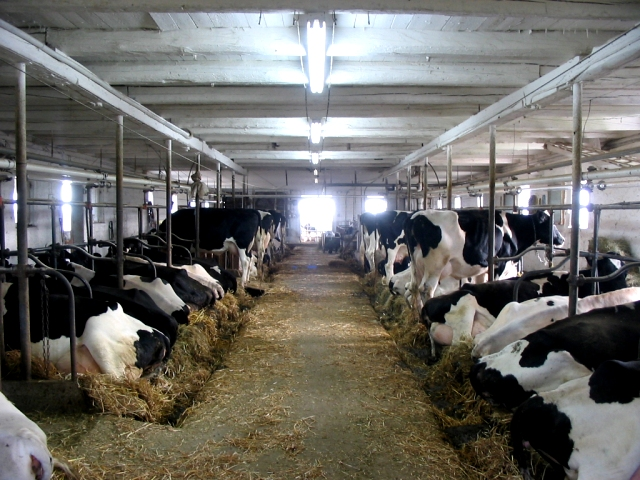
\includegraphics[width = 0.75\textwidth]{figures/tie-stall-barn.jpg}
\caption{Cows in a tie-stall-cowshed \cite{tiestallbarnpicture}. Cows are tied in stall and they are not able to move freely. They also have less space than in a loose-housed cowshed.}
\end{figure}

\begin{figure}
%[thb]
\centering
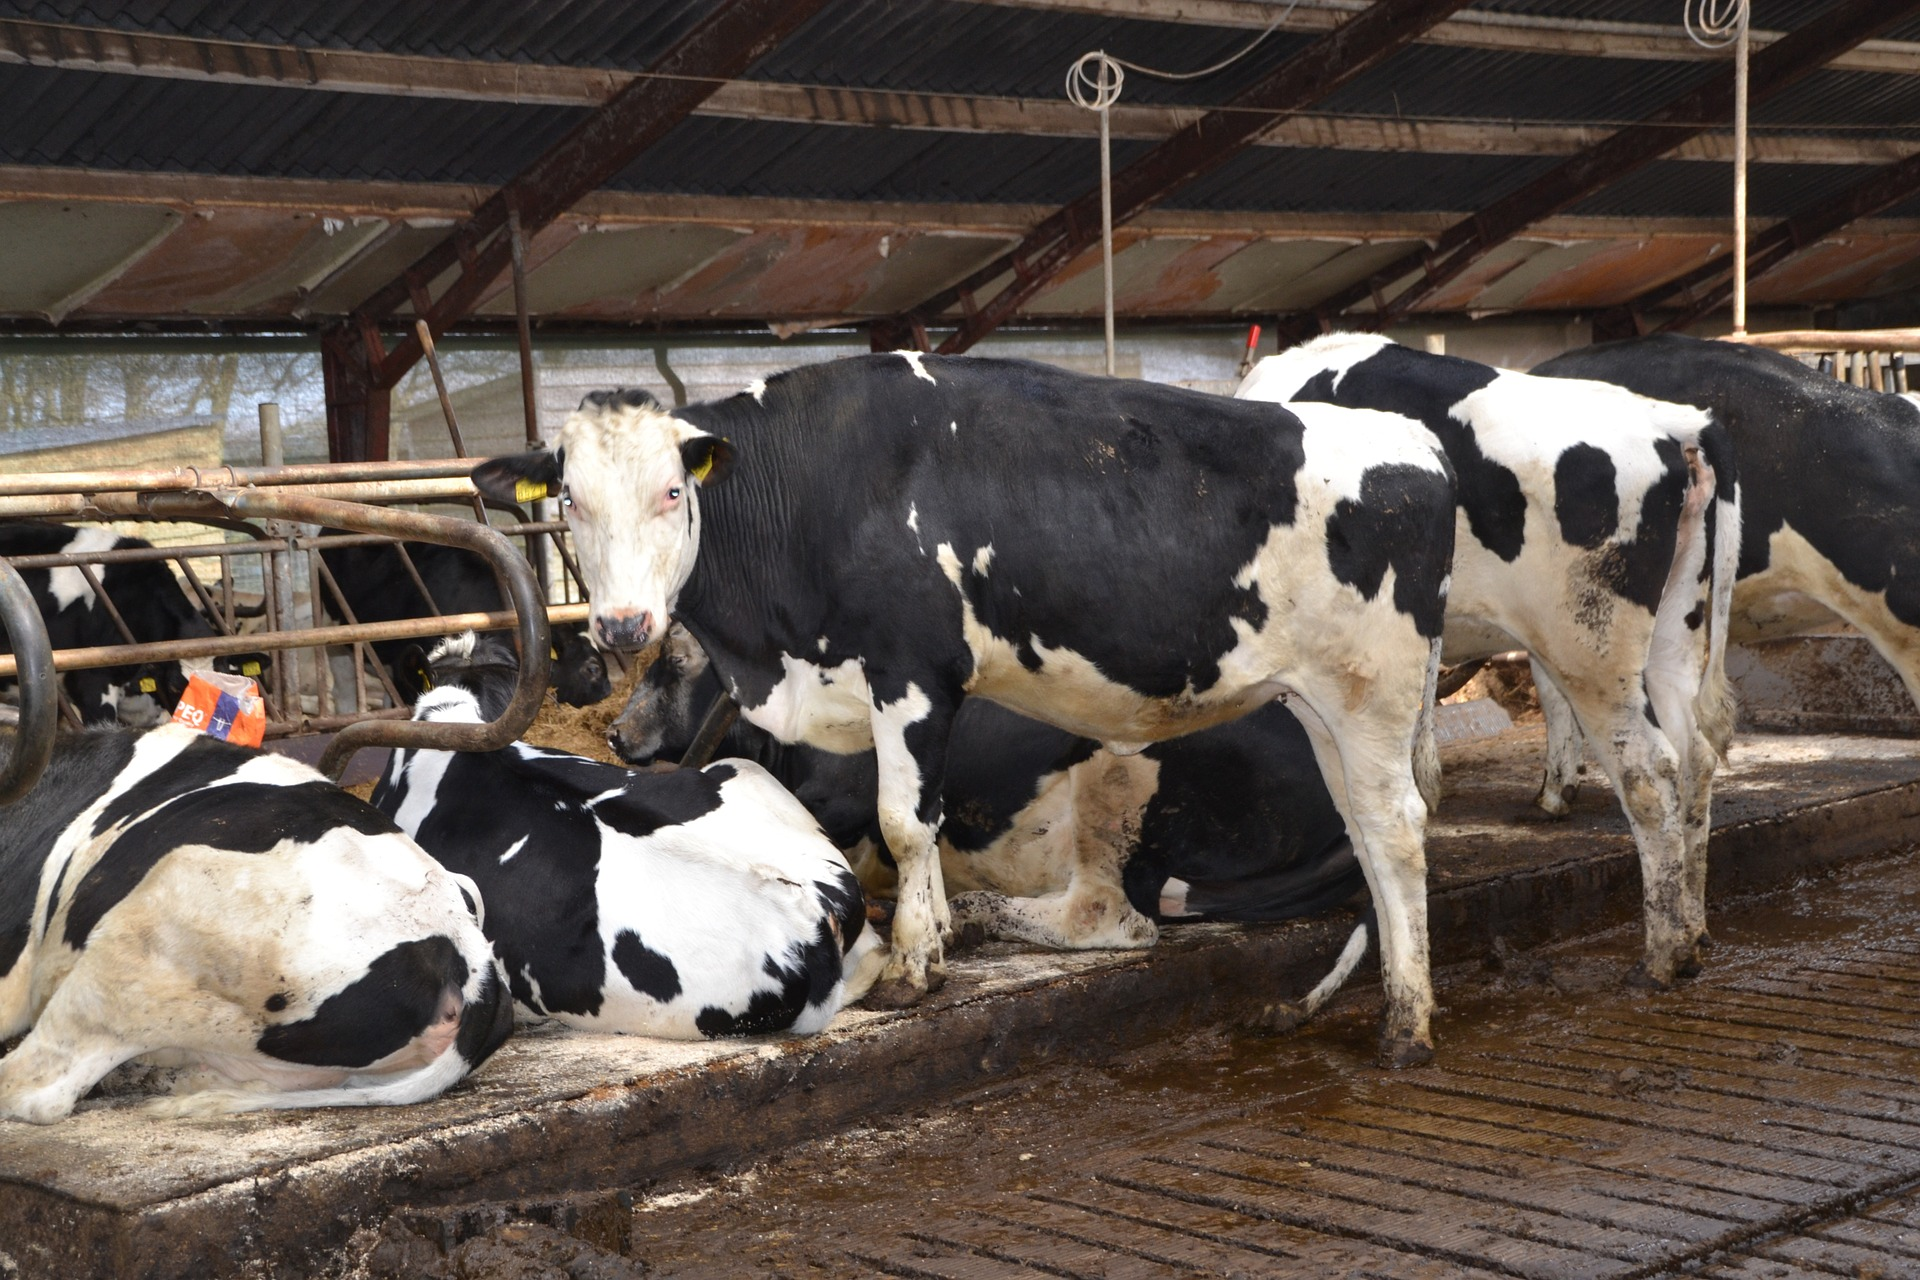
\includegraphics[width = 0.75\textwidth]{figures/free-stall-barn.jpg}
\caption{Cows in a loose-housed-cowshed \cite{freestallbarnpicture}. Cows are able to move freely and act as social animals.}
\end{figure}



\subsubsection{Dairy Cow} \label{dairycowsection}

Tähän alkuun vielä jotakin lehmän perustietoja, kuten arvio rotujen määristä. Lehmän keskimääräinen paino, koskeus, pituus jne. Ehkä myös maininta siitä, kuinka paljon lehmä tarvitsee tilaa mm. laskeutumiseen ja ylösnousuun. 

Previously, we surveyed through the history of animal husbandry and discussed of the beginning milk producing. Additionally, we introduced such cowsheds as tie-stall and loose-housed cowsheds. Correspondingly, this subsection will debate on the dairy cow itself in general level. Whereas, the subsequent subsections will focus on such milk yield related cycles as estrus and lactation cycles. Inherently, cows are plain and herd animals. Moreover, they live in hierarchy \cite{julkaisuja52}. In large herds they form smaller groups where they do their daily activities such as eat and rest together \cite{julkaisuja52} \cite{lehmahavaintoja}. 

Typically, cows lay down approximately from \SI{11}{\hour} to \SI{12}{\hour} every day. Meanwhile, they stand up and change their pose several times \cite{luomunaudanruokinta}. Additionally, they may move their location between haunts and watering places. Thus, in loose-housed cowshed a cow may walk from  \SI{400}{\metre} to \SI{800}{\metre} per day \cite{luomuopas}. On pasture, their daily walking range may extend to several kilometers \cite{luomuopas} \cite{julkaisuja52}. However,  cows are very cautious animals. Thus, insecure circumstances such as slippery ground or high steps can reduce their daily range. Furthermore, cows can be easily injured in challenging places. Naturally, injuries effects to their health and consequently to profitability \cite{lehmahavaintoja}. Nevertheless, Walking enforces the health of them, increases hormonal activity and metabolism \cite{luomuopas}. \\

In addition to their normal activity, cows may have exceptional states. Typically, these states become apparent in their behavior. That is, sicknesses and injuries reduces their activity level, whereas, proestrus increases it. Phases of estrus are covered in detail in section \ref{lactationandestruscyclessection}.

Tänne vähän lisää tietoa lehmien terveysongelmista, kuten ontumisesta, sorkkahommista ja ruoansulatusvaivoista. 

 

 Cow can lick all of its body excluding neck and head. Cows doze standing and sleep lying. The estrus period is approximately 21 days and the estrus lasts from 12 to 16 hours. A bull may detect estrus 2 days before the main estrus.   \cite{julkaisuja52}

 Access to fresh and clean water is vital. \cite{luomuopas} 



\subsubsection{Lactation and Estrus Cycles} \label{lactationandestruscyclessection}

In previous subsections, we discussed of dairy farming and dairy cow in general. Consequently in this section, we will proceed the discussion to lactation cycle. The lactation cycle is emphatically related to the milk yield and thus, the profitability of the farm. The lactation cycle means the period between two calves. Thus, it is also called as calving period. After the calving a cow begins to lactate, which is the the actual purpose of a dairy cow \cite{lehmahavaintoja}. However, the calves are more or less a secondary product in dairy farming and they are not in scope of this study. Nevertheless, the milk yield if a cow increases in the first weeks after the calving. However, after the first weeks the milk yield begins to decrease as illustrated in picture \ref{lactationapproximation}. Consequently, it is not cost-efficient to keep on milking the cow infinitely. Therefore, cyclic calving is preferred in order to maintain the profitability. However, the cow will stop milking before calving which causes a dry period. This causes a dilemma. That is, too short as well as too long calving interval reduces the total milk yield and cuts the profitability. Is general, it is recommended to keep the calving interval roughly in 360 days. Moreover, the milk yield increases after each calving. Thus, it supports the idea of regular calving \cite{lehmientuotoskasvaa}.

 \begin{figure}
 %[thb]
 \centering
 \begin{tikzpicture}
    \begin{axis}[
        xlabel=weeks from calving,
        ylabel=milk yield (kg)]
    \addplot[smooth, blue] plot coordinates {
    	(0,15)
        (1, 30)
        (2, 38)
        (4, 40)
        (6,	39)
        (8,	38)
        (10, 37)
        (12, 35)
        (16, 33)
        (20, 30)
        (24, 27)
        (28, 25)
        (32, 22)
        (36, 21)
        (40, 20)
    };
    \end{axis}
    \end{tikzpicture}
    \caption{An illustrative lactation curve of a dairy cow representing the realtion between the weeks in milk and the milk yield. After the beginning of the lactation, the milk yield reduces in the function of time \cite{lactationcurve}.} \label{lactationapproximation}
 \end{figure}

In recent years, the calving interval has been increasing globally. Alone in Finland, the average calving interval has been extended up to 400 days and it has affected to the milk yield. There has been discussions of the root causes for the extended calving interval. In general, whereas the farm sizes have been increasing the cattle tenders have more work and less time for observing the cows. Thus, it has been more difficult for them to detect any estrus behavior and take actions for insemination. Consequently, this trend has forced the farmers to seek technological aids for punctual estrus detection. Thus, the main scope of this study is in developing of estrus detection algorithms for wearable sensor device. The hardware and software designs are intoruced in section \ref{researchsection} and the results are discussed in \ref{resultssection}. Additionally, we will survey through of currently available solutions in section \ref{currentsolutionssection}.

However, before proceeding to the research of this study, it is necessary to discuss of the estrus cycle of dairy cow. The estrus cycle is the period between ovulations. Actually, the estrus cycle is considered to begin from the ovulation. The normal duration of a cow estrus cycle is approximately 21$\pm$3 days. A bull may detect an estrus already 2 days in advance. The estrus lasts from 12 to 16 hours \cite{julkaisuja52}. The estrus is the time frame when the cow is ready to mate or being inseminated. The estrus is also called as standing heat, hence, the cow allows to being mounted by other cows. Traditionally, being mounted by others has been considered as certain sign of ongoing estrus. Before the estrus, cow has a proestrus period. During the proestrus, cow behaves restlessly and usually it attempts to mount other cows. Normally, cows who are not in estrus do not allow to be mounted. Therefore, these are only attempts and are not considered as a sign of estrus. Typically, the duration of proestrus is from 9 to 18 hours \cite{lehmahavaintoja}.





\subsection{Health Monitoring and Estrus Detection} \label{healthmonitoringandestrusdetectionsection}

The previous subsection \ref{dairyfarmingsection} discussed of the fundamentals of dairy farming. The discussion started form the history of animal husbandry and ended to study of dairy cow itself. The study of dairy cow included basic knowledge of the cow and its environments. Moreover, we discussed of lactation and estrus cycles and their affect on the milk yield and profitability. Additionally, we briefly surveyed through the most common health issues with dairy cow. In continuation to previous discussions, this subsection discusses of different methods for live-stock monitoring. First of the following subsection \ref{currentsolutionssection} surveys through currently used methods and technologies. Correspondingly, the second subsection \ref{researchandstudiessection} discusses of studies of existing technology as well as recent development projects for future solutions.  


\subsubsection{Current Solutions} \label{currentsolutionssection}

Traditionally, live-stock monitoring has been sight-wise task assigned to the cattle tender \cite{lehmahavaintoja}. However, this method is not considered to be efficient. In the USA alone, the rate of successfully detected estruses has been estimated below \SI{50}{\percent} in large farms. Additionally, this inefficiency leads to annual loss of 800 million dollars for the milk industry \cite{BRUNASSI2010}. Naturally, the reliability of the observations depends on several such factors as the experience of the cattle tender, availability of time and the amount of cattle. Additionally, even experienced cattle tender might be erroneous with non-familiar cattle. Furthermore, the head count of farms tend to be increasing whereas the number of cattle tenders remaining the same. Consequently, the tenders have less and less time for purely observing the cattle. Therefore, detection of estrus of health issues has become even more difficult. In despite of the challenges, sight-wise observations by the cattle tender are still common monitoring method in small farms and in developing countries \cite{BRUNASSI2010}. 

Nowadays, there are several commercial poruducts available for dairy cow monitoring. Most typically, these products are sensor devices attached with a strap to leg \cite{iceroboticproductbrochure,geacowscout} or to collar \cite{heatime,geacowscout,moocall} sensor devices are collar or leg devices mounted with straps. \cite{heatime} \cite{iceroboticproductbrochure}. However, there are even tail-attached sensor \cite{moocall} and in rumen \cite{wellcowbolus} sensors available. In addition to various attachments, the devices have various applications. Some sensors are specialized in calving detection \cite{moocall} or digesting monitoring \cite{wellcowbolus} only whereas leg and collar sensors provide more wide range of functionalities. Typically, they monitor the cow motion and activity \cite{iceroboticproductbrochure, heatime, geacowscout, moocall}. Moreover, leg sensors can count steps and detect the pose of the cow (standing, lying and walking). Furthermore, the leg and collar sensors are used in estrus detection. Additionally, some devices are capable of monitoring rumination \cite{heatime} and eating \cite{geacowscout}. Most of the devices are planned for wireless data transmission between the sensor device and a computer of farm server \cite{heatime} \cite{geacowscout} \cite{iceroboticproductbrochure} \cite{wellcowbolus}. However, some devices require wired USB data transmission \cite{iceroboticproductbrochure}. In despite of the technology or the feature being monitored, all the solutions aim to a healthier cow and, thus, improvements in profitability. Others may alert of possible health issues in advance \cite{heatime, geacowscout, iceroboticproductbrochure} whereas others are guiding to optimize the feeding and digestion \cite{wellcowbolus}. Furthermore, numerous current solutions provide mobile phone interfaces ans most significant alerts are given in SMS messages or in email \cite{heatime}.


\subsubsection{Research and Studies} \label{researchandstudiessection}

In former subsection we discussed of currently available technological aids for dairy cow monitoring. Different products provide different functionalities from rumination and digestion monitoring to motion tracking and estrus detection. Similarly in this section, we survey various researches and studies for dairy cow monitoring. In contrast to the previous section, the solutions discussed here are not yet commercially available products. Nevertheless, some studies have been using commercially available devices in their research. In this subsection, our scope will be specially in solutions that are not available in current product range such as behavior monitoring. However, studies of the estrus detection are in our interest as it is the main topic of this study as well. 

Most typically in these researches, the sensor devices are based on various accelerometers \cite{Martiskainen200932} \cite{VazquezDiosdado2015} \cite{Jonsson20116} \cite{Pastell2009545} or pedometers \cite{BRUNASSI2010}. Additionally, such alternative approaches as intravaginal probe has been tested for estrus detection \cite{7370219} \cite{Andersson2016101}. In despite most of the solutions are accelerometer-based, their approach to the topic is quite different. The most complex of these algorithm aims to full behavior detection with support vector machines \cite{Martiskainen200932}. They used an accelerometer based sensor attached to collar of the cow. Their overall performance of the multi-class model was \SI{78}{\percent} precision. However, The precision with lying down and standing up activities were poor. Correspondingly, another research studied use of simple decision tree instead of support vector machines of hidden Markov Models \cite{VazquezDiosdado2015}. In this study, they used various time windows from 1 to 10 minutes. In result, the 1 minute window provided better results than 10 minute window. Additionally, this method was barely equally goon in results as the vector machine algorithms.

Another study used a commercially available leg sensor for estrus detection \cite{Jonsson20116}. From the leg they were able to detect whether the cow was lying, standing or moving. The overall sensitivity in estrus detection was \SI{88.9}{\percent} adn error rate \SI{5.9}{\percent}. Also they used 1 minute sample periods. In this study, the detected estruses were controlled by success of insemination. In their conclusions, they suggested this method could only support existing methods and the reliability is not high enough for standalone solution. Yet another research used pedometers for a step-count based estrus detection \cite{BRUNASSI2010}. In this method they were able to improve the visual estrus detection rate up to \SI{84.2}{\percent}. Also in this study, the estrus detection was verified by the success of insemination. Either this solution was standalone, hence the purpose was use it together with the sight-wise estrus detection. In addition to these accelerometer-based behavior and estrus detection, one research studied lameness detection as attaching one accelerometer to each limb \cite{Pastell2009545}. Their ground idea was sample the accelerometer data from each limb at \SI{25}{\hertz} and use wavelet analysis in order to detect asymmetry, which could be considered as lameness.


In contrast to these more traditional accelerometer-based solution,  another researche studied the use of intravaginal probe for estrus detection \cite{Andersson2016101} \cite{7370219}. The probe was designed to be inserted inter vagina and transmit the temperature and conductivity data wirelessly. The idea for this study was to use non-motion based sensors. Therefore, this solution could be used  also in tie-stall cowshed. The research showed some promising results but lacked of reliability. In their sequel study they used two sizes of the intravaginal probes, \SI{160}{\milli \metre} and \SI{120}{\milli \metre} probes. However, neither of these were successful. The larger probe caused bleeding during the research, whereas the smaller started to rotate and even ejected the vagina. Nevertheless, they were able to found some correlation between the intravaginal temperature as well as the electrical conductivity and estrus.





In behavior based cow monitoring, the sensor devise attempts to recognize on or more of the following acts:

\begin{itemize}
\item \textit{Standing} is a state where the cow stand on all of its legs and stays still.
\item \textit{Lying} is state when the cow lies down on it side. Cows spend half of their day lying down.
\item \textit{Ruminating} is an act where the cow chews the feed from its rumen in order to digest fibers etc.
\item \textit{Feeding} means the act when the cow is eating feed.
\item \textit{Normal walking} when the cow is in health and walks normally.
\item \textit{Lame walking} when the cow has health issues in its legs or claw and its walking is cautions on asymmetrical.
\item \textit{Lying down} means when the cow is standing but changes its state into lying.
\item \textit{Standing up} is when the cow was lying but stands up.
\end{itemize}. The behavior monitoring provides beneficial information for the farmer about the health status as well as the mix of the feed.


\clearpage

\section{Research ok} \label{researchsection}

In previous section \ref{backgroundsection}, we discussed of the essential backgrounds of this study. The discussion started form the beginning of animal husbandry and dairy cow in modern farming. The discussion ended in introduction of currently used methods and survey of recent research and studies. Moreover, the background section focused in milk yield related estrus and lactation cycles in present day farming. In conclusion of the background, there is a certain need for an efficient solutions in dairy cow monitoring. Accordingly, wearable wireless sensor devices are currently the most promising option due their overall performance and availability. Respectively, the target of this study is to develop and evaluate convenient estrus detection algorithms for wearable wireless sensor devices. Therefore, this section discusses of required tools and supportive methods in data recording and algorithm development. Additionally, the data recording software in this study are created from a scratch. Thus, it is necessary to introduce the related software implementations in this study.

In this study, the research section has been divided in three subsections. The first subsections \ref{datarecordingsection}  discusses of data recording. The data records are essential component in algorithm development and evaluation. In this study we will not use already existing data. Thus, we will implement required software as well as record the data for further employment. The subsection introduces the hardware design for the data recording. The hardware discussion covers the main hardware components in reasonable detail. In addition to the hardware design, we discuss of the communication protocols between the main hardware components. Respectively, we introduce the principle work flow of the data recording software. Whereas, the hardware of this study was already existing, the software is self-implemented. Thus, we will discuss of  the implementation more in detail. The second subsection \ref{dataprocessingsection} introduces a set of data processing methods applied on the recorded data. The set of methods consists of basic statistics as well as various digital signal processing tools. In this study, we utilize only the basic statistical analysis and they are introduced briefly. In contrast, the digital signal processing tools are covered in more detailed discussion. Lastly in this section \ref{estrusdetectionalgorithmssection}, we develop three different algorithms for dairy cow estrus detection. All these algorithms have their base in the discussed methods. However, each of the algorithms have their own approach to estrus detection. Nevertheless, all the algorithms detects rather the pro-estrus than the actual estrus \ref{lactationandestruscyclessection}. However, the end of pro-estrus indicates the beginning of the estrus. Therefore, this kind of approach is highly applicable. Additionally, it provides the cattle tender more time to prepare for the required actions. 


\subsection{Data Recording ok} \label{datarecordingsection}

Above, we described the research section of this study in general level. As already stated, this subsection will discuss of the data recording process. The data records are essential components in algorithm development and evaluation. The discussions in this subsection will start from the introduction of data recording hardware. The hardware design in this study is an existing hardware setup. Therefore, we will discuss of the main components and functionalities only superficially. Next, we will discuss of the data recording software. The software for this study is created from a scratch. Therefore, the software design is discussed particularly. In this study, we recorded data in three different occasions of which, the first occasion with a different software implementation. Consequently, we introduce two different software implementation.  Lastly in the data recording subsection, we will describe the actual data recording procedure of all the occasions.


\subsubsection{Hardware ok} \label{hardwaresection}

As stated previously, the data recording hardware in this study is an already existing prototype of a dairy cow sensor device. Originally, the hardware consisted of micro-controller unit (MCU), accelerometer and thermometer. However, it lacked of large enough storage memory for data recording. Thus, the hardware was enhanced with a Secure Digital (SD) memory card slot and with a SD memory card for this study. Otherwise, the hardware design remained the same during the data recording processes. In spite of the mentioned customization, the hardware design is not in the scope of this study. Therefore, the following is rather a description of the hardware than a comprehensive discussion of the design itself. In addition to hardware components, we briefly discuss of the communication between the components. In general, the main hardware components brief descriptions are as follows.

\begin{itemize}
\item \textit{Atmel ATmega32u4} is a high perforamance low power 8-bit micro-controller. It is designed for optimizing power consumption versus processing performance. It contains 135 powerful Reduced Instruction Set Computer (RISC) architecture instructions of which most executable in a single clock cycle.  \cite{atmega32u4datasheet} 

\item \textit{Bosch Sensortec BMA222E} is an accelerometer with on-chip motion triggered interrupt controller. Thus, it enables motion-based applications even without utilizing a micro-controller. It is capable of measuring acceleration in three perpendicular axises. BMA222E is designed for various consumer products from game controllers to pedometers. It is small sized and low power consuming. Therefore, it is suitable for mobile battery-powered solutions.  \cite{bma222datasheet} 

\item \textit{Texas Instruments TMP112} is a high-accuracy, low-power, digital temperature sensor. It is designed for various applications from portable and battery-powered solutions to general temperature merasurements in industrial controls. \cite{tmp112datasheet} 

\item \textit{Secure Digital (SD)} memory card is specially designed to meet the security, capacity and performance requirements in newly emerging consumer electronic devices. The standard capacity of SD memory card is up to \SI{2}{\giga\byte}. However, High Capacity SD (SDHC) extends the maximum capacity to \SI{32}{\giga\byte} and Extended Capacity SD (SDXC) up to \SI{2}{\tera\byte}. \cite{sdspecification}. In this study, the maximum capacity of SDHC card shall be considered as the maximum available memory capacity. This restriction shall be taken into considerations while designing the sensor software. Moreover, the memory card shall be capable of recording one estrus cycle at minimum (approximately 21 days).

\end{itemize} In addition to the hardware components, the hardware configurations utilizes two serial interfaces, \textit{inter-inegrated circuit (I$^2$C) bus} and \textit{serial peripheral interface (SPI)}. They are explained briefly in the following.

\begin{itemize}
\item \textit{Inter-Inegrated Circuit (I$^2$C) bus} which is some times referred as \textit{Two-Wire Interface (TWI)} is a serial communication interface developed by Philips Semiconductor. The first version of  the I$^2$C was released in 1982. The design of it is rather simple hence, it requires only only two bidirectional open-drain lines, Serial Data Line (SDA) and Serial Clock Line (SCL), with pull-up resistors \cite{i2cmanual}.


\item \textit{Serial peripheral interface (SPI)} \cite{spimanual} is a more complex serial interface than the (I$^2$C) bus. It requires at minimum of three parallel wires in three-wire mode \cite{bma222datasheet} \textit{signal select} ($\bar{SS}$), \textit{serial clock} (SCK) and \textit{serial data input/output} (SDI). However, in normal four-wire mode the data input and output are in separate lines, \textit{master out, slave in} (MOSI) and \textit{master in, slave out} (MISO).
\end{itemize}  As we have now introduced the main components of the sensor device, the communication principles of the device are represented in figure \ref{serialdiagram}. As shown in the picture, SD memory card utilizes SPI serial interface whereas temperature sensor and accelerometer are connected into same I$^2$C bus. Naturally, all of these hardware components are assigned to their specific tasks with respect to their functional description. Therefore, their essential functionalities are discussed in the following topics.

\tikzstyle{vecArrow} = [thick,
   decoration={markings,mark=at position
   1 with {\arrow[semithick]{open triangle 60}}},
   double distance=2.4pt, shorten >= 5.5pt,
   preaction = {decorate},
   postaction = {draw,line width=1.4pt, white,shorten >= 4.5pt}]  
\tikzstyle{dvecArrow} = [thick,
   decoration={markings,mark=at position 0 with {\arrow[rotate=180, semithick]{open triangle 60}}},
   decoration={markings,mark=at position 1 with {\arrow[semithick]{open triangle 60}}},
   double distance=2.4pt,
   shorten >= 5.5pt,
   shorten <=5.5pt,
   preaction = {decorate},
   postaction = {draw,line width=1.4pt, white,shorten >= 4.5pt}]  
\tikzstyle{innerWhite} = [semithick, white,line width=2.4pt, shorten >= 4.5pt]
\tikzstyle{dinnerWhite} = [semithick, white,line width=2.4pt, shorten >= 4.5pt, shorten <= 4.5pt]


\begin{figure}
\centering
\begin{tikzpicture}[thick]
  \node[draw,rectangle, minimum width = 6em, minimum height = 10em] (ATMEGA) {ATmega32u4};
  \node[inner sep=0,minimum size=0,left of=ATMEGA, node distance = 10em] (LEFT) {}; % invisible node
  \node[inner sep=0,minimum size=0,right of=ATMEGA, node distance = 5em] (RIGHT) {}; % invisible node
  \node[draw, rectangle, minimum width = 5em, above of=LEFT, node distance = 3.5em, minimum height = 3em] (TMP) {TMP112};
  \node[draw, rectangle, minimum width = 5em, below of=LEFT, node distance = 3.5em, minimum height = 3em] (BMA) {BMA222e};
  \node[draw, rectangle, minimum width = 5em, right of = RIGHT, node distance = 5em, minimum height = 3em] (SD) {SD-card};
  \node[] at (-5.25em,1em) {I$^2$C};
  \node[] at (5.25em,1em) {SPI};
  \draw[dvecArrow] (TMP) to (BMA);
  \draw[dvecArrow] (ATMEGA) to (SD);
  \draw[vecArrow] (LEFT) to (ATMEGA);
  \draw[dinnerWhite] (TMP) to (BMA);
  \draw[dinnerWhite] (ATMEGA) to (SD);
  \draw[innerWhite] (LEFT) to (ATMEGA);
\end{tikzpicture}
\caption{The principal block diagram of the sensor device. The temperature sensor and accelerometer are connected to the micro-controller via the same I$^2$C-bus, whereas, SD-card is connected via SPI-bus. Power connections nor USB are not represented in this figure.}
\label{serialdiagram}
\end{figure}


\subsubsection*{Micro-controller ok}

The \textit{micro-controller unit (MCU)} is the core component of the sensors device in this study. That is, the micro-controller is responsible of execution of the software flow whenever the device is powered. Typically, the first executable task in the software flow is the system initialization. Normally, system is initialized once in software flow and each time after resetting or starting the micro-controller. During the initialization, the micro-controller sets up its control register according to the configurations in its program memory. These registers contains the configurations for the \textit{general purpose input output} (GPIO) pin configurations as well as timers, serial interfaces and other featured functionalities. In addition to self configuration, the micro-controller initializes connected hardware via serial interfaces according to the configurations in the software memory. Next, after initialization the micro-controller begins the execution of the actual software flow. Typically, this flow is a repetitive software loop including variable tasks and events. The hardware initialization and configurations as well as the application tasks and events are discussed more the software section \ref{softwaresection}.

As discussed earlier, Atmel ATmega32u4 \cite{atmega32u4datasheet} is the micro-controller unit of the sensor device in this study. It is a high performance, low power micro-controller for various applications. Therefore, we will discuss of its features and functionalities more in detail. In spite of the wide range of its features, only the most fundamental properties are covered in the following discussion.


\begin{itemize}
\item \textit{\SI{32}{\kilo\byte} of In-System Self-Programmable Flash memory} is the memory space for the actual program storage. Furthermore, the memory space is divided into two sections, Boot program Section and application Program section. 

\item \textit{USB 2.0 Full-Speed/Low-speed Device Module} provides interface to write on the in-system self-programmable flash memory of the controller. Thus, it enables uploading the application software without external USB module. Additionally, the interface contributes serial communication between computer and the device.

\item \textit{General I/O} consists of 26 programmable I/O lines. These lines can be set as input or output separately. Furthermore, specific input pins can be configured as interrupt pins. Typically, interrupts are utilized for triggering events in the software flow. Additionally, interrupts are also a required feature in serial communication events.

\item \textit{Interrupts} are occasions that usually set an interrupt flag. Next, the \textit{interrupt service routine (ISR)} corresponding the interrupt flag is executed with respect to its priority. Optionally, it is possible to execute a task directly in the interrupt. However, it temporarily disables other interrupts, hence, it is not recommended. Furthermore, there are internal and external interrupts. The source of internal interrupts are inside the micro-controller itself, as timers. Correspondingly, the source of external interrupts are external devices such as sensors or memory storages. Additionally, the interrupt can be enabled individually. The main advantage of utilizing interrupts is to execute tasks on-demand instead of periodically.

\item \textit{Watchdog Timer (WDT)} of ATmega32U4 employs a separate on-chip \SI{128}{\kilo \hertz} oscillator for creating timer events. If the WDT is enabled it is capable of resetting the entire micro-controller unless, the WDT is not reset regularly. Normally, WDT is utilized for recovering from deadlocks, unintentional conditions without exit. However, it is possible to utilize the watchdog timer as a wake-up timer in low power modes.


\item \textit{Power Management and Sleep Modes} allows the user to tailor the power consumption according the application requirements. Power management is beneficial feature specially with battery-powered solutions when regular re-charging is not effortless to accomplish.

\item \textit{SPI and I$^2$C} serial bus interfaces are used for device-internal communication of the micro-controller and the sensors as well as the SD memory card. The serial interfaces were briefly discussed in section \ref{hardwaresection}.

\end{itemize}


\subsubsection*{Accelerometer ok}

As discussed previously, a micro-controller is the core component of the hardware design of the sensor device. Similarly, an accelerometer is the essential sensors providing data for data recording as well as algorithm development. In this study, the utilized accelerometer is the Bosch Sensortech BMA222E \cite{bma222datasheet}. It is a triple-axial accelerometer used for measuring the change in the motion. Additionally, it can be employed in position recognition in constant situations. The axises of the accelerometer are perpendicular. Therefore, it is capable of measuring in all direction. Additionally, it contains several advantageous on-chip functions. It is capable of prior and post filtering acceleration measurements. Additionally, it can detect various conditions and trigger interrupts in result. Moreover, the filters as well as the detectable conditions are highly configurable. These configurations are discussed in the following description. Nevertheless, the accelerometer contains several functionalities without use-cases in this study. Consequently, those features are not covered in the discussions. However, some of the features have no direct use case in this study but are applicable in the future studies that are considered in section \ref{conclusionssection}. Additionally, the sensor configurations varies between two software implementations in this study and they are discussed in the sectin \ref{softwaresection}. The kay features of the BMA222E accelerometer are as follows.


\begin{itemize}
\item \textit{On-chip interrupt controller} is capable of generating  interrupts from various conditions. The conditions are configurable with respect to time or numerous motion statuses. On-chip interrupt controller yields an opportunity to create device applications even without a micro-controller. However, in this study all the interrupts are processed in the micro-controller. Nevertheless, the interrupt controller is utilized to create favorable sampling events instead of continuous sample recording.

\item \textit{On-Chip FIFO Register} is capable of storing up to 32 data frames. Depending on the configurations, one frame contains measurements from chosen or all three axis. Additionally, it is configurable whether the data in the register is filtered or unfiltered. Furthermore, the register contains information whether the data is new or old data.

\item \textit{Range} of the acceleration measurements is adjustable within four preset ranges,  $\pm$\SI{2}{\gram}, $\pm$\SI{4}{\gram}, $\pm$\SI{8}{\gram} and $\pm$\SI{16}{\gram}. However, increasing the range decreases the resolution and vice versa. Thus, selecting of appropriate range shall be considered.

\item \textit{8-bit Resolution} is applicable for both, acceleration and temperature measurements. As discussed, the range of acceleration measurements is adjustable and affects the resolution. Consequently, the resolution is from \SI{15.63}{\milli\gram} per \textit{least significant bit (LSB)} to \SI{125}{\milli\gram} per LSB. The  Nevertheless, the temperature resolution is fixed to \SI{0.5}{\celsius} per LSB.

\item \textit{Low Pass Filter} enables removing of high frequency distortion from the measured signals. Thus, no additional low pass filtering is needed in the micro-controller application. The low pass filter of the accelerometer is configurable with preset frequencies from $7.81$ Hz to $1000$ Hz. The bandwidth configuration effects the interval, how frequently, new data frame is readable from the register of the sensor. Roughly, the values are update twice often than the filter bandwidth according the Shannon-Nyquist sampling theorem.

\item \textit{Offset Compensation} allows removing offsets from the measured signals. At sea level, there is always approximately \SI{1}{\gram} offset present. Specially in integrative calculations the presence of offset accumulates and yield misleading results.


\item \textit{SPI and I$^2$C digital interfaces} are necessary interfaces for configuring the sensor as well as data transmission from the accelerometer from the micro-controller. It is configurable, which interface is utilized.

\item \textit{Low Power Consumption} is beneficial in portable and battery-powered solutions such as the sensor device in this study. Additionally, the accelerometer enables improvement of the power consumption with several power modes. However, the power modes are not applicable in this study because, one of the core ideas is to utilize the accelerometer as effectively as possible instead of more  power consuming micro-controller.
 
\item \textit{On-chip Temperature sensor} of the controller provides a resolution of \SI{0.5}{\celsius}. The accuracy of the BMA222E is relatively low in comparison to the TMP112 temperature sensor discussed later in this section. Nevertheless, it is useful as a reference or verification value with the measurements of the TMP112 temperature sensor. \cite{bma222datasheet}

\end{itemize}



\subsubsection*{Temperature Sensor ok}

Whereas the accelerometer is the main sensor of the sensor device, a temperature sensor is considered as a supportive sensor. Furthermore, the accelerometer contains a built-in temperature sensor. However, its resolution is relatively low. In contrast, Texas Instruments TMP112 is a high-accuracy temperature sensor for various applications from portable devices to industrial controls.  It is specially designed for replacing \textit{negative temperature coefficient (NTC)} and \textit{positive temperature coefficient (PTC)} thermistors in high accuracy applications. In this study, the temperature sensor is used for monitoring the skin temperature of the cow. The target of the monitoring is to find correlation between the change of skin temperature and ongoing estrus or pro-estrus. Therefore, in the case of positive correlation the temperature sensor can confirm the detected estrus. In contrast, a negative correlation can confuse the results and yield a need for further studies. The properties of the TMP112 temperature sensor are described in the following.


\begin{itemize}
\item \textit{High accuracy} of 

\begin{itemize}
\item \SI{0.5}{\celsius} in range from \SI{0}{\celsius} to \SI{65}{\celsius}

\item \SI{1.0}{\celsius} in range from \SI{-40}{\celsius} to \SI{125}{\celsius}
\end{itemize} 

without calibration. Furthermore, instructions for the calibration of the sensor are provided in the data sheet. 

\item \textit{High resolution} of \SI{0.0625}{\celsius} in both, 12-bit and 13-bit modes

\item \textit{Low power consumption} in two different power modes:
\begin{itemize}
\item \SI{10}{\micro \ampere} in active mode
\item \SI{1}{\micro \ampere} in shutdown mode
\end{itemize}

\item SMBus\textsuperscript{TM}, Tow-Wire and I$^2$C digital interfaces

\item supply voltage range from \SI{1.4}{\volt} to \SI{3.6}{\volt}

\item \textit{Conversion rate} from \SI{0.5}{\hertz}  to \SI{8}{\hertz}

\item \textit{12-bit resolution} from \SI{-55}{\celsius} to \SI{128}{\celsius}. The sensor has an 13-bit mode, when the measu
rement range is up to \SI{150}{\celsius}. \cite{tmp112datasheet}
\end{itemize} In this study, the temperature sensor is soldered directly on the circuit board. In result, the sensor is not in direct skin contact with the cow. Therefore, the skin temperature is conducted from skin to the sensor via heat conducting aluminum tape.

%\subsubsection*{Secure Digital Memory Card}

%As discussed above, suitable data storage was not initially included in the data recording hardware. Therefore, the original design was enhanced with a secure digital memory card slot for replaceable memory card. The purpose of the SD card is functioning as a long term data storage. Naturally, it is supposed to be capable of record data for more than one estrus cycle (approximately 22 days). The final requirements for appropriate card size depends on the sampling interval as well as the format the data is recorded on the card. Therefore, it is reasonable to estimate the required memory size after the device application software is implemented. Nevertheless, the maximum capacity the high capacity secure digital memory cards of \SI{32}{\giga\byte} shall be considered as the maximum. Thus, the software implementation shall adopt to this maximum memory limit.



\subsubsection{Software ok} \label{softwaresection}

As discussed in previous section, the data recording hardware in this study is a prototype of dairy cow sensor device enhanced with memory card slot. By contrast to the hardware, the data recording software had to be implemented from a scratch for this study. Therefore, this section will discuss of the software design as well as the software implementation.  Additionally, we will introduce the software development tools utilized in this study. The design phase of the software development included hardware test for defining the restrictions and capabilities. Consequently, it slowed the design process. Nevertheless, hardware test results that had no effect are not included in the results of this study. However, after proper testing and design, the actual software implementation was rather straight forward process. In this section we will first introduce rduino Integrated Development Environment (Arduino IDE) \cite{arduinoide} as our primary software tool in application development. Next, we will present two different software implementations. The first software implementation was utilized as a test and the results were mainly used in for software improvement. Consequently, the second software implementation differs from the first one and is more optimized for long term data recording. Lastly in this software section we will discuss of the data recording procedures. In the following we have short description of Arduino IDE and of its utilized libraries.


\begin{itemize}
\item \textit{Arduino IDE} provides a fast and easy software development environment for implementing micro-controller applications without prior expert-level knowledge on micro-controllers. Additionally, Arduino and Arduino community supports with comprehensive set of software libraries for various micro-controller applications.

\item \textit{Wire} library provides functionality for Inter-Integrated Circuit (I2C) communication. "This library allows you to communicate with I2C / TWI devices. On the Arduino boards with the R3 layout (1.0 pinout), the SDA (data line) and SCL (clock line) are on the pin headers close to the AREF pin. The Arduino Due has two I2C / TWI interfaces SDA1 and SCL1 are near to the AREF pin and the additional one is on pins 20 and 21." \cite{arduinowire}

\item \textit{SPI} library provides the interface for uitlizing of SPI bus for inter-integrated chip communication. Furthermore, Arduino's IDE library provides functionalities for both, master and slave devices \cite{arduinospi}. Nevertheless, in this study the sensor device shall work as a master. 

\item \textit{SD} library allows reading from and writing to SD cards. The library supports FAT16 and FAT32 file systems on standard SD cards and SDHC cards. It uses short 8.3 names for files. That is, eight characters for filename and three for extension. \cite{arduinosd}

\item \textit{EnableInterrupt} library provides interface for configuring interrupt pins. In additoin to enabling and disabling the interrupts, interrupt conditions e.g. rising edge, faling edge, low are configurable. \cite{arduinoenableinterrupt}

\item \textit{RingBuf} is a library for simple \textit{first in first out (FIFO)} buffers for the Arduino. Buffers created with the library can buffer any fixed size object such as ints, floats and structs. \cite{arduinoringbuf}
\end{itemize} In addition to the standard libraries, Arduino community provides plenty of open-source software libraries for various applications. In spite of the numerous software libraries, they do not comprehensively include all the functionalities of the supported micro-controllers. Therefore, a profound familiarization with the micro-controller data sheet is mandatory step in order to achieve the optimal performance of the controller. However, the Arduino programming language is merely a set of C/C++ functions. Thus, it enables of implementation of ad-hoc functions such as hardware configurations. In this study, this flexibility was utilized in driver implementation for the accelerometer and temperature sensor since, their original drivers were not correctly supported in Arduini IDE. Furthermore, the data logging interface was created from s scratch. In result, there are two different log types in this study, one for each software implementation. Nevertheless, in both cases, the logs are written on SD-card on common .txt-files. In the following subtopics, we will discuss both software implementations in detail.




\subsubsection*{First Software Implementation ok}\label{firstdatasetconfigurations}


% Define block styles
\tikzstyle{decision} = [diamond, draw,, aspect=2, fill=blue!20, 
    text width=7.5em, text badly centered, node distance=2.5cm, inner sep=0pt]  
\tikzstyle{block} = [rectangle, draw, fill=blue!20, 
    text width=5em, text centered, node distance=2.5cm, rounded corners, minimum height=4em]   
\tikzstyle{invisible} = [inner sep=0,minimum size=0, node distance = 2.5cm]
\tikzstyle{line} = [draw, -latex']
\tikzstyle{cloud} = [draw, ellipse,fill=red!20, node distance=2.5cm,
    minimum height=2em]
    
\begin{figure}
\centering
\begin{tikzpicture}[node distance = 2.0cm, auto]
    \node [block] (INIT) {Initialize};
    \node [cloud, left of = INIT, node distance = 4cm] (START) {Start};
    \node [decision, below of = INIT] (INTERRUPT) {Interrupt};
    \node [block, right of = INTERRUPT, node distance = 5cm] (READACC) {Read acceleration data};
    \node [decision, below of = READACC] (SAVEDATA) {Save data};
    \node [block, below of=SAVEDATA] (SAVETOSD) {Save data to SD-card};
    \node [invisible, left of = SAVEDATA] (MID2) {};
    \node [invisible, left of = SAVEDATA, node distance = 5cm] (MID1) {};
    \node [invisible, left of = SAVETOSD, node distance = 5cm] (MID6) {};
    \node [invisible, below of = MID6, node distance = 1.5cm] (MID10) {};
    \node [decision, below of = MID10, node distance = 1.5cm] (TIMER) {Timer};
    \node [invisible, below of = TIMER, node distance =1.5 cm] (MID7) {};
    \node [decision, below of = MID7, node distance = 1.5 cm] (TIMEOUT) {Timeout};
    \node [invisible, below of = TIMEOUT, node distance = 1.5 cm] (MID8) {};
    \node [decision, below of = MID8, node distance = 1.5 cm] (ERRORS) {Errors};
    \node [invisible, below of = ERRORS, node distance = 1.5cm] (MID9) {};
    \node [decision, below of = MID9, node distance = 1.5cm] (BUFFER) {Buffer empty}; 
    \node [block, right of = TIMER, node distance = 5 cm] (READTEMP) {Read Temperature};
    \node [block, right of = TIMEOUT, node distance = 5 cm] (SETFLAG) {Set interrupt flag};
    \node [block, right of = BUFFER, node distance = 5 cm] (WRITEDATA) {Write buffer to SD-card};
    \node [block, right of = ERRORS, node distance = 5 cm] (HANDLE) {Handle errors}; 
    \node [invisible, left of = BUFFER, node distance = 4cm] (MID4) {};
    \node [invisible, left of = INTERRUPT, node distance = 4cm] (MID5) {};
    \node [invisible, below of = WRITEDATA, node distance = 1.75] (MID11){};
    \node [invisible, below of = MID4, node distance = 1.5 cm] (MID12){};
    \path [line] (INIT) -- (INTERRUPT);
    \path [line] (START) -- (INIT);
    \path [line] (INTERRUPT) -- node {true}(READACC);
    \path [line] (READACC) -- (SAVEDATA);
    \path [line] (SAVEDATA) -- node {true}(SAVETOSD);
    \path [draw] (SAVEDATA) -- node[above] {false} (MID2);
    \path [line] (MID2) -- (MID1);
    \path [line] (SAVETOSD) |- (MID10); 
    \path [draw] (INTERRUPT) --  node[left]{false}(MID1);
    \path [line] (MID1) -- (TIMER);   
    \path [draw] (TIMER) -- node [left]{false} (MID7);
    \path [line] (MID7) -- (TIMEOUT);
    \path [draw] (TIMEOUT) -- node [left]{false} (MID8);
    \path [line] (MID8) -- (ERRORS);
    \path [draw] (ERRORS) -- node [left]{false} (MID9);
    \path [line] (MID9) -- (BUFFER);   
    \path [line] (TIMER) -- node[above] {true} (READTEMP);
    \path [line] (READTEMP) |- (MID7);
    \path [line] (TIMEOUT) -- node{true} (SETFLAG);
    \path [line] (SETFLAG) |- (MID8);   
    \path [line] (BUFFER) -- node {false} (WRITEDATA);
    \path [line] (ERRORS) -- node {true} (HANDLE);
    \path [line] (HANDLE) |- (MID9);
    \path [line] (BUFFER) -- node[above] {true}(MID4);
    \path [draw] (MID4) -- (MID5);
	\path [line] (MID5) -- (INTERRUPT);    
    \path [draw] (WRITEDATA) |- (MID12);
    \path [draw] (MID12) -- (MID4) ; 
\end{tikzpicture}
\caption{The software flow of the first data recording software. The rounded rectangles represents tasks whereas the diamonds are conditions. Each condition is followed by branches depending on the current situation. The tasks and conditions form a repetitive loop of executions excluding the initialize task.}
\label{softwareflow1}
\end{figure}

In this study, it was considered that software implementation based on strict initial assumptions could impair the the achieved results. Therefore, the approach for the first software implementation was to avoid utilizing unnecessary  or defective functionalities of the accelerometer. In conclusion, it was decided to prioritize high sampling rate over other features. Specially, irreversible pre-processes should be avoided. Thus, e.g. offset compensation was not in use in this software implementation. Furthermore, the offset data can provide vital information of the pose of the sensor. Nevertheless, the data was low-pass filtered in order to avoid the folding of frequencies higher than the half of the sampling rate. The maximum sampling rate of the accelerometer is limited in \SI{2000}{\hertz}. Consequently, the minimum update time is \SI{0.5}{\milli\second}. However, utilizing a filter douples the update time if filtered values are configured as output values. In spite of the high sampling rate of the accelerometer, the usage of secure digital (SD) memory card as a data storage limits the data rate rather effectively. That is, the duration of the SD file operations such as open, write and close exceeds the disposable time at high data rate. In result, it causes the FIFO buffers of the accelerometer to overflow. Consequently, undefined amount of data is lost. In contrast, a low sampling rate could cause a loss of possibly relevant features on higher frequencies. Therefore, the optimization of the data rate is more or less a trade of between data and feature losses.

The software flow of the first data recording software is represented in figure \ref{softwareflow1}. The flowchart consists of tasks (rounded rectangles) and conditions (diamonds). A condition is s state with two or more possible exit branches. In this study, the conditions are of Boolean type with only two following branches. In contrast, tasks are executable functions typically between conditions. Nevertheless, a branch may include a sequence of conditions as well as sequence of beaches. Furthermore, a task might contain smaller tasks and smaller conditions whereas conditions may contain smaller tasks and smaller conditions. Nevertheless, the conditions presented in the flowchart are discussed in the following itemization.


\begin{itemize}
\item \textit{Interrupt} is true if an interrupt flag is set by an interrupt from the accelerometer which in this case is a certain FIFO buffer level.

\item \textit{Timer} condition is used for reading temperature data from both of the sensors periodically. The temperature variation is not a high frequency process. Therefore, it is rather reasonable to read temperature values more seldom than accelerometer data.

\item \textit{Timeout} is a backup condition in the case of missed interrupt from the accelerometer. That is, the accelerometer gives FIFO level interrupt only once, unless the micro-controller reads it empty after receiving the interrupt. Therefore, if micro-controller misses the interrupt it will not receive a new one. In consequence, it can cause a deadlock situation.

\item \textit{Errors} condition is for handling of the detecting errors in the software flow. The detectable errors need to be defined. The purpose of error detection is mainly improving the software and evaluation the quality of the recorded data.

\item \textit{Buffer empty} condition checks the buffer level of the micro-controller. If the buffer level is more than zero the values in the buffer will be written to the text file on the SD card.

\item \textit{Save data} condition detects s safe timing for performing save data task. The save data task includes time consuming SD-card file operations such as close file and open file.

\end{itemize}
Correspondingly, the software flow contains the following tasks.

\begin{itemize}

\item \textit{Initialize} task (which is analogous for \textit{setup} function in Arduino IDE) is executed only once right after the device is powered up. This task initializes the micro-controller itself as well as the desired configurations for the accelerometer and the temperature sensor.

\item \textit{Read acceleration data} task reads all the data from the FIFO buffer of the accelerometer and stores the it into the FIFO buffer of the micro-controller. Actually, the serial interface is capable of transmitting less than six data frames at a time. Therefore, the task reads sets of five data frames until there are more than zero but less than five frames available. Lastly, the task reads the remaining frames. In result, the FIFO buffer of the accelerometer should be apty.

\item \textit{Save Data to SD-card} task saves the data written on the SD card. According to the Arduino's SD library, the written data is saved only after the file is closed utilizing the close function. Otherwise, the data will be lost and it is not possible to recover it afterwards. Additionally, in order to continue fluent writing process, the save data task re-opens the file. However, if the size of the log file exceeds the set maximum file size, the save data task will open a new log file. Furthermore, the duration of the open and close file operations could exceed the time required to fill up the FIFO buffer of the accelerometer. Thus, the FIFO buffer is being read empty before and after closing the current file and once more after opening a file. 

\item \textit{Read temperatures} task reads the temperature data of both sensors and stores the value to the memory of the micro-controller. No temperature data are buffered. Thus, only the latest values are written on the log file on the SD-card.

\item \textit{Set Interrupt flag} sets the interrupt flag without an interrupt if a timeout condition is met. Once the interrupt flag is set, the micro-controller will read the acceleration data from the FIFO buffer of the accelerometer. Consequently, it is possible for the accelerometer to set new interrupt flag once its FIFO buffer is being filled.

\item \textit{Handle errors} task handles predefined errors if one or more of them have occurred. In practice, this task writes the names of the occurred errors into the text file and resets all of the error flags.

\item \textit{Write buffer to SD-card} writes a single line of acceleration data from the FIFO buffer of the micro-controller into a text-file on the SD card. However, in normal execution of the software flow, all conditions are most likely false. In result, the software will sequentially write multiple lines of acceleration data before another condition is met.
\end{itemize}





\subsubsection*{Second Software Implementation ok}\label{seconddatasetconfigurations}


\begin{figure}
\centering
\begin{tikzpicture}[node distance = 2.0cm, auto]
    \node [block] (INIT) {Initialize};
    \node [cloud, left of = INIT, node distance = 4cm] (START) {Start};
    \node [decision, below of = INIT] (FIFO) {FIFO-level > 0};
    \node [invisible, below of = FIFO, node distance = 1.5 cm] (MID4) {};
    \node [decision, below of = MID4, node distance = 1.5 cm] (WDT) {WDT flag};
    \node [block, right of = WDT, node distance = 5 cm] (GETTEMP) {Read Temperature};
    \node [block, below of = GETTEMP] (OPENFILE) {Open file};
    \node [block, below of = OPENFILE] (WRITEDATA) {Write data to file};
    \node [block, below of = WRITEDATA] (CLOSEFILE) {Close file};
    \node [invisible, left of = CLOSEFILE, node distance = 5cm] (MID5) {};
    \node [decision, below of = MID5, node distance = 1.5 cm] (FIFO2) {FIFO-level > 0};
    \node [block, below of = FIFO2] (SLEEP) {Sleep};
    \node [invisible, left of = FIFO2, node distance = 4 cm] (MID2) {};
    \node [invisible, below of = WDT] (MID3) {};
    \node [block, right of = FIFO, node distance = 5 cm] (READACC) {Read acceleration};
    \node [invisible, left of = SLEEP, node distance = 4 cm] (MID6) {};
    \path [line] (START) -- (INIT);
    \path [line] (INIT) -- (FIFO);
    \path [draw] (FIFO) -- node[left]{false}(MID4);
    \path [line] (MID4) -- (WDT);
    \path [draw] (WDT) -- node [left]{false}(MID3);
    \path [line] (WDT) -- node{true}(GETTEMP);
    \path [line] (MID3) -- (FIFO2);
    \path [line] (FIFO) -- node{true}(READACC);
    \path [line] (READACC) |- (MID4);
    \path [line] (GETTEMP) -- (OPENFILE);
    \path [line] (OPENFILE) -- (WRITEDATA);
    \path [line] (WRITEDATA) -- (CLOSEFILE);
    \path [line] (CLOSEFILE) -- (MID5);
    \path [line] (FIFO2) -- node[left]{false}(SLEEP);
    \path [line] (FIFO2) -- node[above]{true}(MID2);
    \path [line] (MID2) |- (FIFO);
    \path [draw] (SLEEP) -- node [above]{wake up}(MID6);
    \path [draw] (MID6) -- (MID2);
\end{tikzpicture}
\caption{The program flow of the second data logging software}
\label{softwareflow2}
\end{figure}
Whereas the first software implementation was created without descent pre-knowledge, the second software implementation benefits from the results of the first data set. As discussed in the results section \ref{generalresultssection} the first data set experienced multiple lost data frames. Furthermore, the frequency analysis showed there is no need for high frequency sampling. Actually, most of the frequency spectrum was less than \SI{8}{\hertz}. Therefore, the approach in this second software implementation is in improving the performance. The focus is specially in avoiding lost data frames. Additionally, a secondary target is reducing the device lifetime considering the battery and memory card capacities. However, battery or memory card capacities were not issues with the first data set. Nevertheless, the improvements are beneficial with possible future studies as well. The flowchart of the second software implementation is represented in figure \ref{softwareflow2}. In comparison to the first implementation, the software design is rather simple in the design level. That is, the second implementation consist of only three conditions whereas the first was designed with six. Furthermore, the number of tasks is reduced by one. Additionally, the task are in sequence without intermediate conditions. The conditions of the second software implementation are described in the following itemization.

 
\begin{itemize}
\item \textit{FIFO-level > 0} condition is true if the FIFO buffer level of the accelerometer is non-zero.

\item \textit{WDT flag} condition is true if the watchdog timer has set a watchdog timer (WDT) flag.
\end{itemize}
Correspondingly, the tasks of the second software implementation are as follows.


\begin{itemize}
\item \textit{Initialize} task initializes the micro-controller as well as the other components of the sensor device.

\item \textit{Read acceleration} task reads all the data from the FIFO buffer of the accelerometer and stores the data into the FIFO buffer of the micro-controller.

\item \textit{Read temperature} task reads the temperature of both of the sensors, accelerometer and temperature sensor.

\item \textit{Open file} task opens a file for writing the data. The task opens a new file if the size of the current file exceeds a preset limit for maximum file size.

\item \textit{Write data to file} writes all the buffered acceleration data into the opened file on the SD card. In addition, the task writes the temperatures of both of the sensors, the number of occurred watchdog timer interrupts and the up-time of the micro-controller into the text file.

\item \textit{Close file} task closes the opened file in order to ensure the written data is being saved. 

\item \textit{Sleep} task sets the micro-controller into a power saving mode. That is, all the other functionalities except the watchdog timer and interrupts are disabled in order to minimize the power consumption. The micro-controller remains in the sleep until the watchdog timer or an interrupt from the accelerometer wakes up the micro-controller. After waking up, the continues the execution of the software flow from the beginning of the repetitive loop.

\end{itemize}

\subsubsection{Procedure ok} \label{proceduresection}

Previously we discussed of the software implementations for the data recording. In this section we will discuss of the actual data recording process on real dairy cow farm. The farm utilized in this study is located in coordinates N\ang{63;6;3.6} E\ang{23;10;35.5}. The breed of the farm contained of Ayrshire and Holstein cows and they both are used in data recording. The data was recorded in total of three separate occasions. First of the sessions was recorded with the first software implementation whereas the last two with the second software implementation. The recording of the first data set was started on Friday September the 9\textsuperscript{th} at the target farm. The sensor device was attached to the collar of the selected cow. The target of the first data recording was acquiring initial information of the cows behavior as well as performing frequency analysis of the data. Therefore, the cows was equipped also with additional trail camera. A  \SI{8}{\giga \byte} SD-memory card was used as a log file storage during this occasion. Initially it was estimated to sustain approximately 16 days, hence, the recording required approximately \SI{500}{\mega \byte} per a day. The recording of the first data set was ended on Sunday September the 18\textsuperscript{th}. After removing the devices from from the collar, all the log files as well as trail camera images were stored on computer for further studies. These results are discussed in results section \ref{resultssection}.

In contrast to the first data recording event, total of three devices were used on the second and third sessions. In addition to the increased number of devices, the sensor software was improved considering the capacity of data storage and batteries. In result, the memory storage was estimated to sustain roughly for 500 days and batteries at least 60 days. Furthermore, a video camera was mounted on the ceiling of the barn during the second data recording event. Nevertheless, the memory of the camera was fulfilled in 24 hours. The purpose of the video camera was similar to the trail camera in the first session, searching correlation between motion data and the video based behavior monitoring. During the third data recording event, no video devices were used. The second data set was recorded on the test farm from December the 14\textsuperscript{th} to 15\textsuperscript{th}. Meanwhile this data was analyzed and algorithms developed, the third data set was recorded until January the 20\textsuperscript{th}. In addition to the data recording sensors, the cow were equipped with Heatime cow monitoring system. This system was utilized as a reference for the estrus detection algorithms. Figure \ref{sensorikaulassakuva} illustrates the cow with a collar sensor. Additionally, the axises of the accelerometer are shown in the picture. In addition to the picture of cow wearing the sensor, figure \ref{heatconductingtape} shows the heat conducting tape on the bottom side of the sensor device. This aluminum tape is in continuous skin contact with the cow and conducts the heat to the temperature sensor on the circuit board. Furthermore, differences between the software implementations are represented in table \ref{softwareparameterstable}. Additionally, table contains information of fundamental performance estimation.



\begin{figure}[thb]
\centering
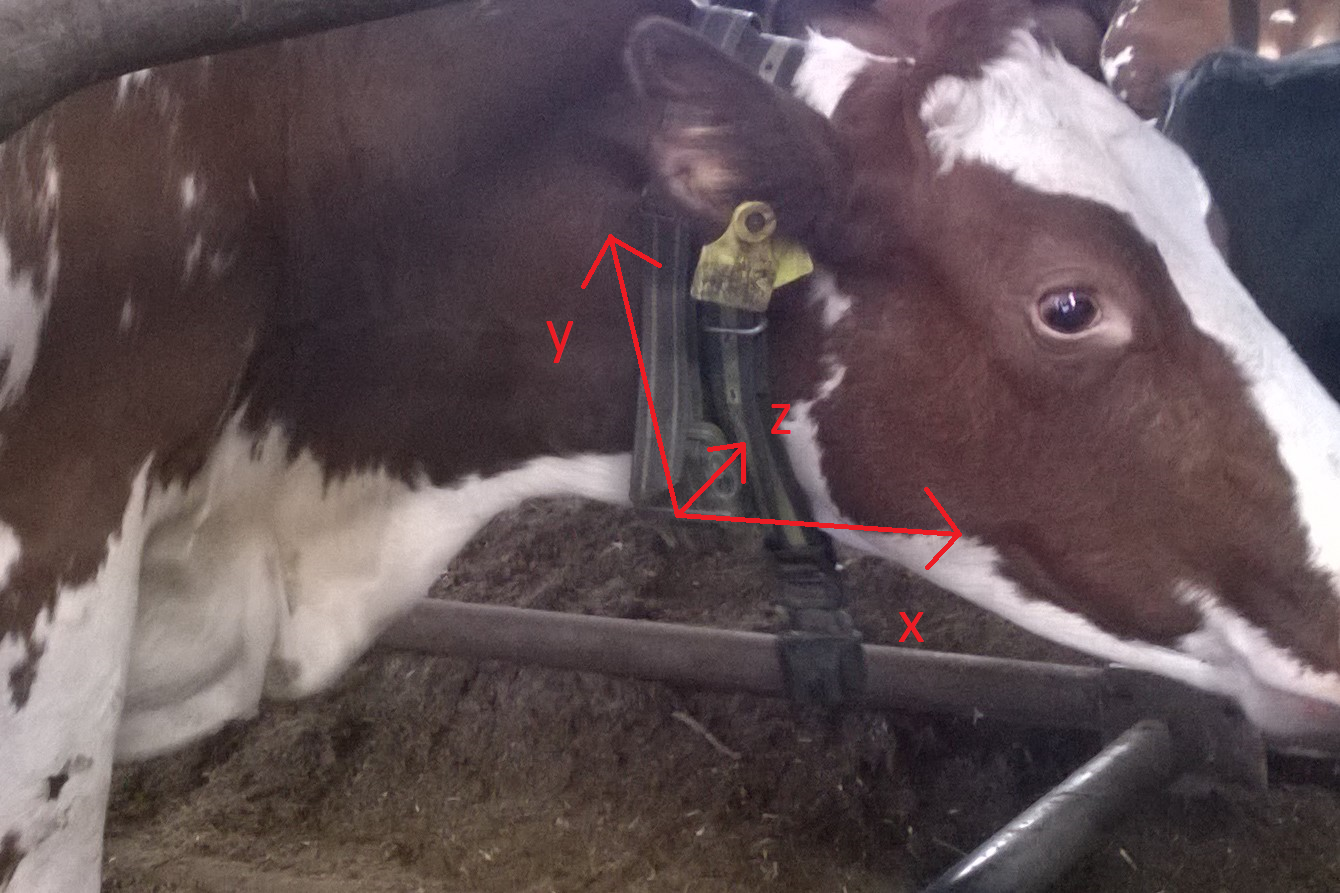
\includegraphics[width = 0.75 \textwidth]{figures/sensorikaulassa1.png}
\caption{Cow wearing a sensor device. The axis directions are illustrated with the red arrows in the figure. The sensor is in parallel with a commercial Heatime device also seen in this figure.}\label{sensorikaulassakuva}
\end{figure}


\begin{figure}[thb]
\centering
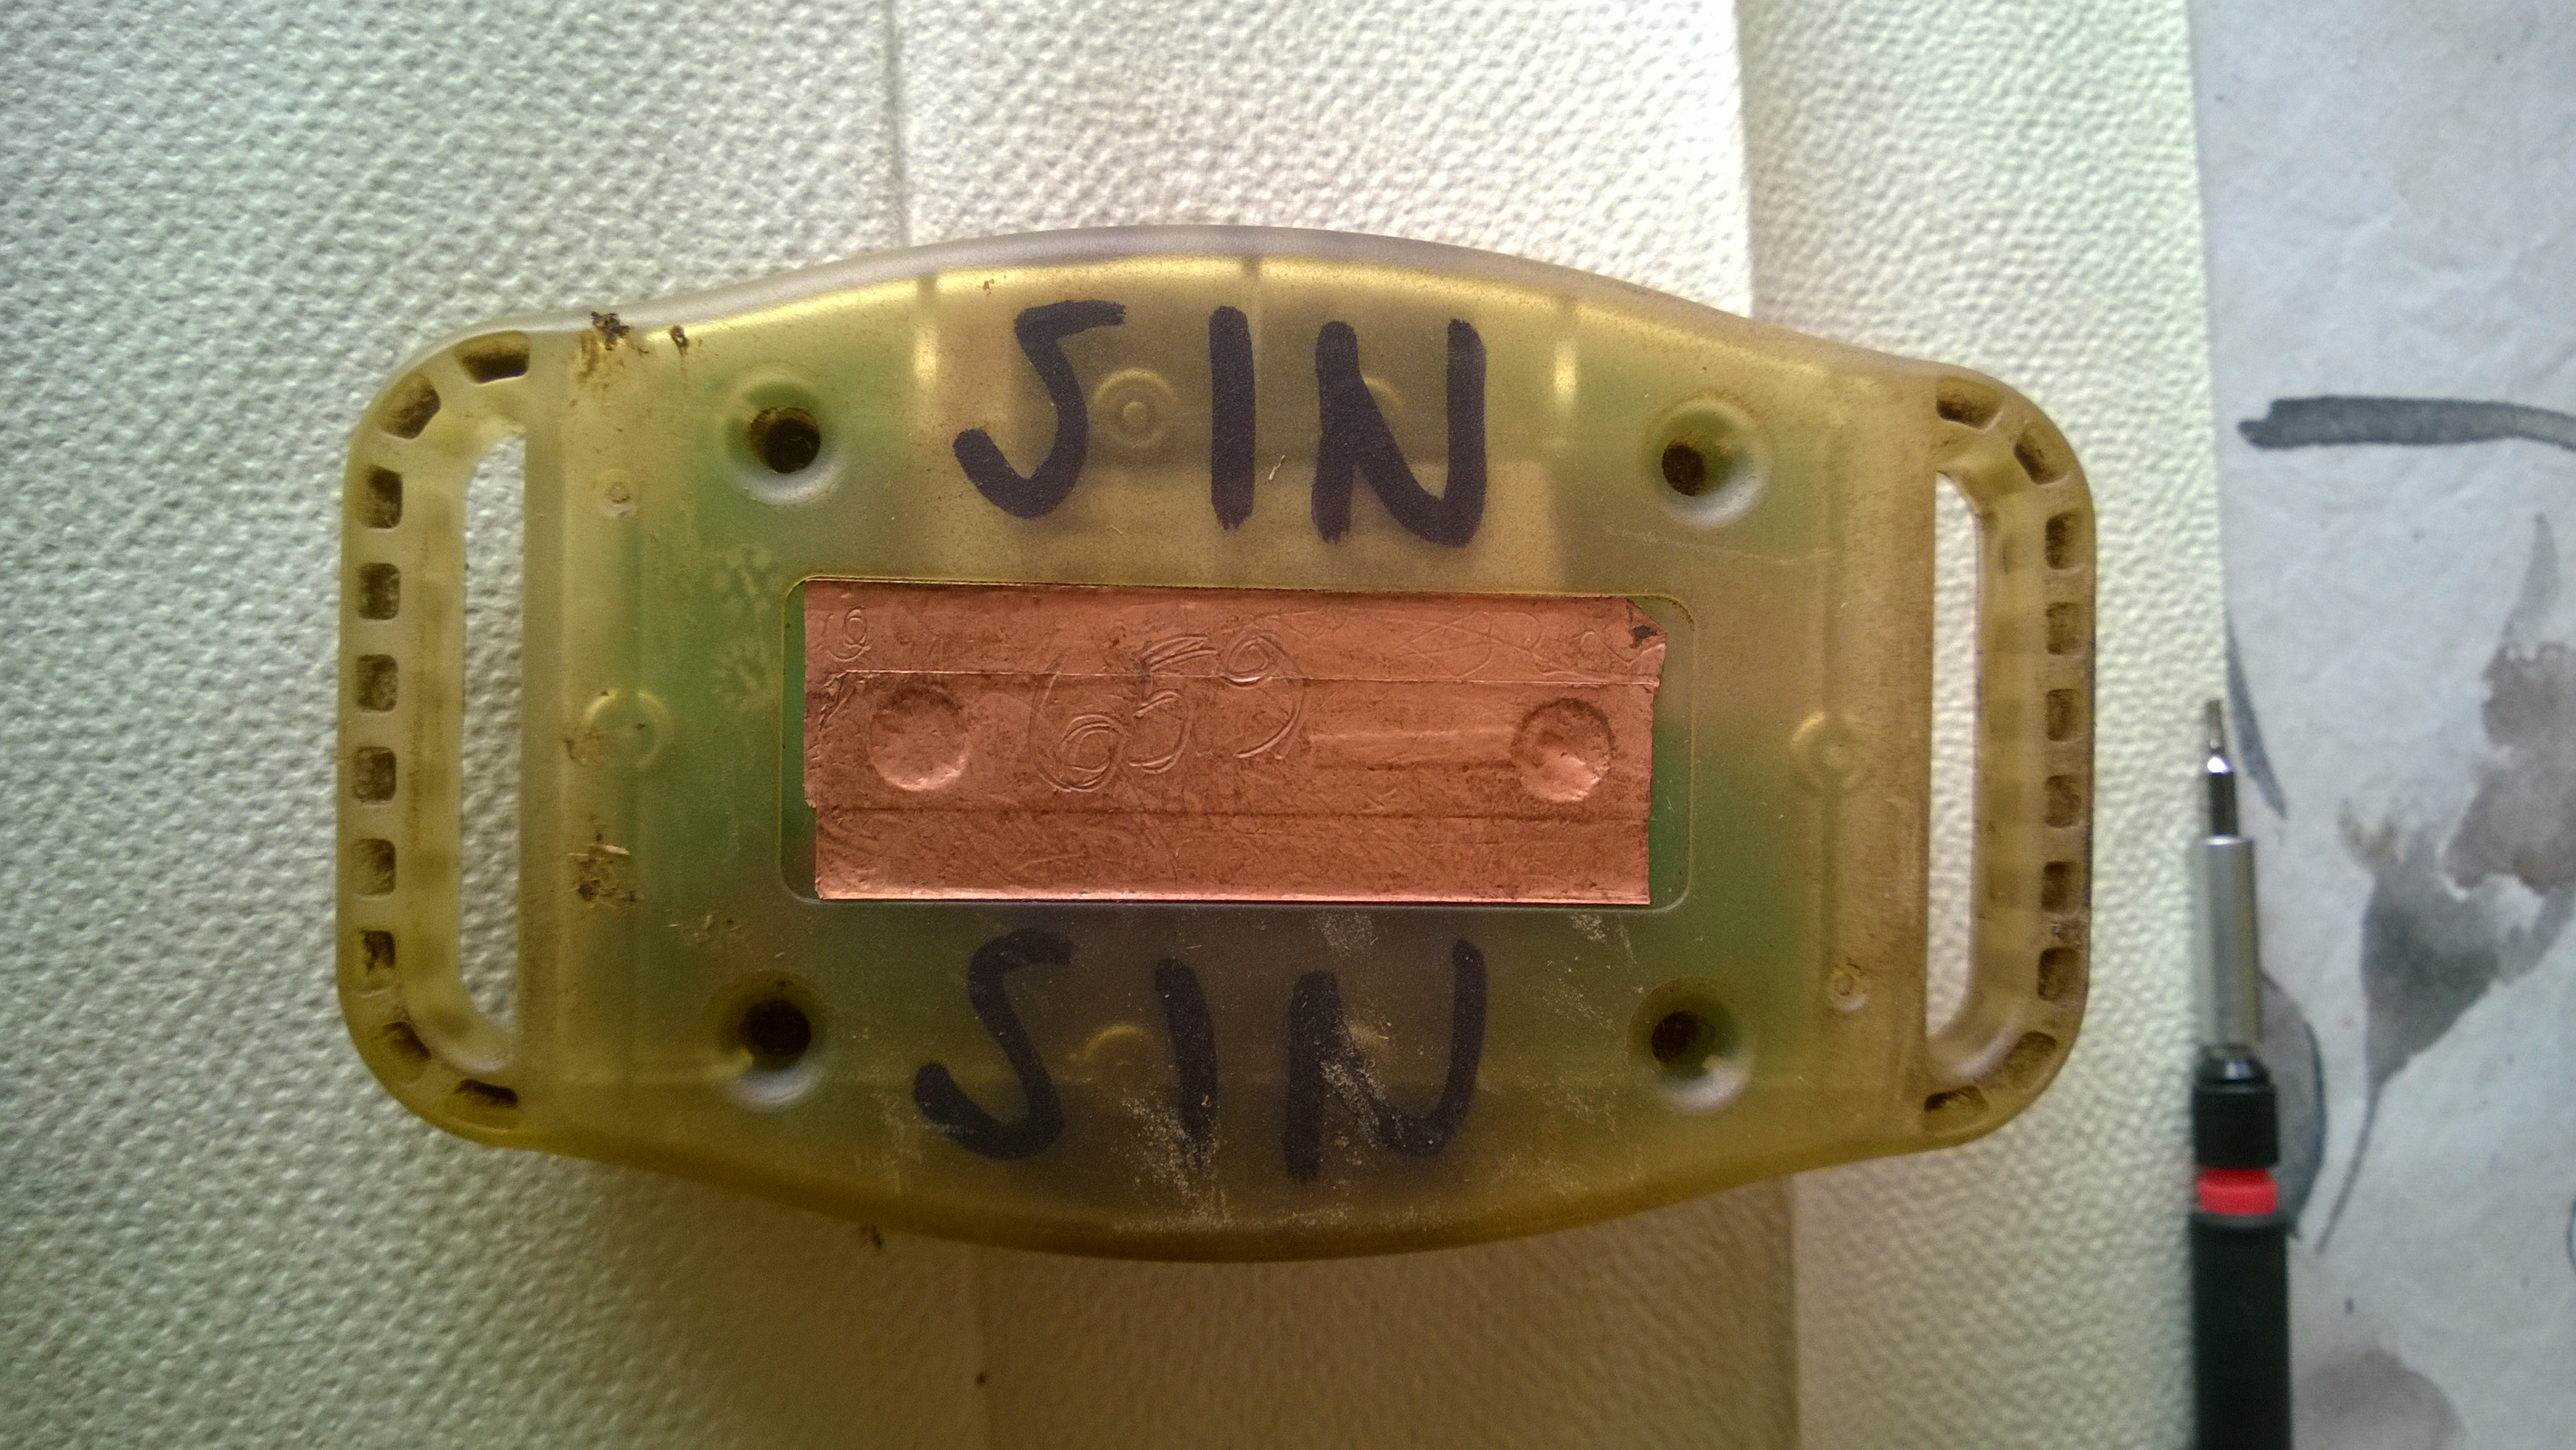
\includegraphics[width = 0.75 \textwidth]{figures/heatConductingTape.jpg}
\caption{The heat conducting tape on the bottom-side of the sensor device. The purpose of the tape is conducting the skin temperature of the cow to the temperature sensor on the circuit board.}\label{heatconductingtape}
\end{figure}



\begin{table} \caption{Data recording parameters of different data recording occasions and software implementation} \label{softwareparameterstable}
\centering
\begin{tabular}{| p{6.25cm} | p{3cm} | p{3cm} |}
\hline
\textbf{Parameter name} & \textbf{First software implementation} & \textbf{Second Software Implementation} \\  \hline
Low-pass filter bandwidth & \SI{125}{\hertz} & \SI{7.81}{\hertz} \\ \hline
Update interval & \SI{4}{\milli\second} & \SI{64}{\milli\second} \\ \hline
Measurement range & $\pm$\SI{4}{\gram} & $\pm$\SI{8}{\gram} \\ \hline
Accelerometer buffer size & 20 & 30 \\ \hline
Interrupt latching & \SI{12.5}{\milli\second} & latched \\ \hline
Internal Buffer Size & 200 frames & 200 frames \\ \hline
SD-memory card size & \SI{8}{\giga\byte} & \SI{16}{\giga\byte}  \\ \hline
estimated SD-capacity & approx. 16 days & approx. 500 days \\ \hline
\end{tabular}
\end{table}




\subsection{Data Processing ok} \label{dataprocessingsection}

Previously, we have been discussing of the data recording hardware and software as well as the data recording process itself. Accordingly, this section focuses in the data processing methods. The data processing methods consists of basic statistics as well as such digital signal processing methods as \textit{fast Fourier transform (FFT)} and digital filters. Thus, the discussion in this section will start from the most essential statistic methods. Second, we will study the Fourier transform as a tool fro the frequency analysis. Third, we discuss of digital filters. The discussion rest of the fact the accelerometer includes filter for distortion attenuation as well as offset compensation. Last, in this section we introduce a sliding window as an essential principle while processing large amounts of data.

However, prior processing of the data, it is essential to parse the data from log files into applicable form. In this study, we use \textit{MathWorks MATLAB} (later Matlab) \cite{matlaboverview} software for both, log file parsing and data processing. Furthermore, the format of log files varied depending on the software implementation. Therefore, corresponding data parsing scripts are required. In the log files, the data is written as certain rows containing the desired information. The purpose of the data parsing script is to convert the data from text characters into numeric values. Furthermore, the secondary purpose of the data parser is in reorganizing the data into practical structures for the future purposes. Additionally, the amount of data in log files was as minimal as reasonable. However, the paring sequence is capable to compute additional values such as time and include that into the structs for further purposes. In spite of these computational data processing methods, plotting and visual observation is the essential method in algorithms development as well as in feature identification.

\subsubsection{Statistics ok} \label{statisticssection}

As already discussed, the data processing methods in this study consists of various tools. The statistics is an effective method of describing large amounts of data in few characteristics. Furthermore, they are relatively easy to compute. Therefore, statistics are one of the fundamental data processing tools in this study. Additionally, the statistics are deployed in several sequences from prior analysis to the various phases of estrus detection algorithms. In spite of the benefits of advanced statistics, in this study we use only the most essential statistical characters. The utilized statistical numbers are discussed in the following itemization \cite{maoltaulukotmatematiikka}.

\begin{itemize}
\item \textit{Mean} is an average value that attempts to describe the most typical value of the data set. However, mean is sensitive to unevenly and asymmetrically distributed values. Therefore, in such cases median is more valuable depicting the most typical value. Nevertheless,  mean is defined as the sum of all values divided the number of values as in the following equation.
\begin{equation} \label{meanequation}
\bar{x} = \frac{\displaystyle \sum\limits^{n}_{i = 1} x(i)}{n}
\end{equation} 

\item \textit{Median} also describes the most common value of the data. In contrast to the mean, it is not that sensitive to unevenly and asymmetrically distributed values. Therfore, it is more applicable when data contains such features as large peaks Median is defined as the middlemost value of sorted data. If the number of values in the data is even, the median is the mean of the two middlemost values.

\item \textit{Variance} describes the expectation of the squared deviation of a random variable from its mean, and it informally measures how far a set of (random) numbers are spread out from the mean:
\begin{equation} \label{varianceequation}
s^2 = \frac{ \sum\limits_{i = 1}^{n}(x(i) - \bar{x})^2}{n}
\end{equation} 

\item \textit{Standard deviation} describes the amount of variation in the data set. A low standard deviation means the values tend to be close to the mean value, whereas a high value means the values tend to be far from the mean. In contrast to the variance, the standard deviation describes the ``typical''  distance between the values and the mean. The standard deviation is actually the square root of variance:
\begin{equation} \label{standarddeviationequation}
s = \sqrt{\frac{ \sum\limits_{i = 1}^{n}(x(i) - \bar{x})^2}{n}}
\end{equation}

\item \textit{Minimum} is the smallest value in the data set.

\item \textit{Maximum} is the largest value in the data set.

\item \textit{Range} is the absolute difference between the minimum and the maximum values.
\end{itemize}





\subsubsection{Fourier Transform ok} \label{fouriertransformsection}

Frequency analysis of a signal is fundamental phase in filter design as well as in adjustment of the sampling rate. According to the Shannon-Nyquist theorem, the minimum sampling rate shall be at least twice the signal frequency. Otherwise, high frequency components may fold over the lower frequencies and distort the signal. In this study, we did not make initial assumptions of the signal frequency of the acceleration signal. Thus, the sampling frequency was set as high as possible. The purpose is to use the frequency analysis to choose more suitable low-pass filter bandwidth for the second data recording application. Nevertheless, understanding of frequency analysis requires understanding of periodic signals. The basis of fourier transform is in Fourier analysis. That is, in the seventeenth century mathematician Jean Baptiste Fourier discovered that periodic signals could be approximated as series of simple sine and cosine functions. In fact, the Fourer transform is linear mapping of a signal from time domain into frequency domain. COrrespondingly, inverse Fourier transform is inverse linear mapping from frequency to time domain. Continuous time Fourier transform is representend in equation \ref{fouriertransformequation} \cite{khan2005digital}. 


\begin{equation} \label{fouriertransformequation}
\hat{f}(\omega) =  \int_{- \infty} ^{\infty} f(x) ^{-i\omega x} \mathrm{d}x
\end{equation}  
Similarly as normal Fourier transform, textit{Discrete Fourier transform (DFT)} is also linear mapping of a signal from time domain to frequency domain. However, continuous time equations apply on continuous time signals whereas discrete time equations on discrete signals. Corresponding discrete time Fourier transform is represented in equation \ref{fftequation}.

\begin{equation} \label{fftequation}
F_n =  \sum \limits^{N-1}_{k=0} f_k e^{-i(2\pi k / N) n} \mathrm{\hspace{1em} , n = 0, \dots , N -1} 
\end{equation} 
Normally, DFT would require approximately $n^2$ iterations for mapping the time domain to the frequency domain. With large samples this becomes mathematically demanding and time consuming process. Therefore, there are alternative approaches called Fast Fourier Transforms (FFT). They require less computing and time, approximately only $n \log n$ iterations. In practice, the fast Fourier Transform is solved numerically instead of solving it mathematically. However, the results may not be as exact as it is with DFT \cite{khan2005digital} \cite{rao2012fast}. Nevertheless, in this study we will use the FFT functions included in the standard libraries of Matlab software \cite{matlabfft}. The theoretical background of FFT is rather profound and therefore, it is not in the scope of this study. The fft function of Matlab does not actually consider frequency at all. In contrast, it provides only a numeric solution. Therefore, corresponding frequency vector needs to be created and mapped manually to the solution. Otherwise, the fft function of Matlab is fast and rather straightforward function.

%Nevertheless, we will briefly discuss of the use of the fft function of Maltab as follows.

%For the fft, it is required to define the length of the sample as well as the sampling frequency. Next, we will create a vector with frequencies from zero to half of the sampling frequency. Actually, the fft of the Matlab does not straight consider the true frequencies. Therefore, the user himself need to set the frequencies correctly. The fft function results the frequency data in complex numbers. Therefore, it is required to get the absolute value of the results. Yet, the the results are two sided data. Thus, we need to exclude the other half of it. Lastly, we correct the amplitude and plot the resulting vector with the frequency vector we created earlier. \cite{matlabfft}.




\subsubsection{Digital Filters ok} \label{digitalfilterssection}

Filters are one of the fundamental tools in signal processing. Properly designed filter removes such undesired components from the signal as distortion and offset. Typically signal is smoother after applying a filter. Typically, filters are applied in the beginning of the signal processing sequence. However, there are no restrictions of applying filters in multiple phases of the sequence. In general, filters can be divided in four different types, low-pass, high-pass, band-pass and band-stop filters. Low-pass filters are desirable in removing high-frequency components. Normally, the purpose is removing of distortion. Usually, in these cases the source of distortion is external and not a part of the original phenomenon e.g. mechanical vibrations, acoustic and electrical noises. Similarly, high-pass filters are applied when low frequency components e.g. offset and DC voltage are not in the focus of the current application. Furthermore, band-pass and band-stop filters are special combinations of low-pass and high-pass filters. Band-pass filters are designed to pass only specific frequency band and removing components below and above it. Conversely, band-stop filter is design for filtering only a specific frequency band and allowing other frequencies to pass. \cite{digitalfilters} \cite{khan2005digital}

Filters can also be separated as analog and digital filters. Analog filters are based on a physical combination of analog electrical components such as resistors, capacitors and inductances. In contrast, digital filters are a sequence of arithmetic operations. Consequently, digital filters can be implemented on specific digital circuits or in software applications. Nevertheless, analog filters are usually present also in digital applications as preliminary and protective filters prior digital sampling. Specially, it is crucial to filter out frequency components above the Nyquist frequency in order to void folding. In this study, we will concentrate only on digital filters. Furthermore, the approach is to imitate the filters inside the Bosch Sensortec BMA222E accelerometer. The Accelerometer contains two configurable on chip filters, 2nd order low-pass filter and 1st order high-pass filter \cite{bma222datasheet}. The bandwidth of the low-pass filter is configured directly via the control register of the sensor. However, the high-pass offset compensating filer depends on the selected bandwidth of the low-pass filter as well as specific preset. That is, the cutoff frequency of the high-pass filter is either one-hundredth or one-thousandth of the low-pass cutoff frequency. Unfortunately, the data sheet of the sensor did not provide further information of the filters except the filter order. Therefore, these filters are replicated in this study based on the available information.

Digital filters can be divided into two categories, \textit{finite impulse response (FIR)} filters and \textit{infinite impulse response (IIR)} filters. The topology of FIR filter is represented in figure \ref{firfilterdiagram} whereas the topology of IIR filter is shown in figure \ref{iirfilterdiagram}. The names of the filters follow their impulse response. The FIR filter has a finite impulse response whereas the impulse response of IIR filter is infinite. As seen in the FIR filter equation \ref{firequation}, the output of the filter is dependent on only current and previous input signal levels. Therefore, the output signal cannot be longer than the degree of the filter. By contrast, the IIR filter is also dependent on its own current and previous outputs as seen in the equation \ref{iirequation}. Thus, if the filter is stable it converges but never reaches absolute zero after an impulse input.



\begin{figure}[htb]
\centering
\begin{tikzpicture}
% Place nodes using a matrix
	\matrix (m1) [row sep=2.5mm, column sep=5mm]
	{		%--------------------------------------------------------------------
		\node[dspnodeopen,dsp/label=above] (m00) {$x[n]$}; &
		\node[coordinate] (m01) {}; &
		\node[dspnodefull] (m02) {}; &
		\node[coordinate] (m03) {}; &
		\node[dspgainr] (m04) {$b_0$}; &
		\node[coordinate] (m05) {}; & 
		\node[dspadder]	(m06) {}; &
		\node[coordinate] (m07) {}; &
		\node[dspnodeopen,dsp/label=above] (m0X) {$y[n]$}; 
		\\
	%--------------------------------------------------------------------
		\node[coordinate] (m10) {}; &
		\node[coordinate] (m11) {}; &
		\node[dspsquare] (m12) {$\z^{-1}$}; &
		\node[coordinate] (m13) {} ; &
		\node[coordinate] (m14) {};          &
		\node[coordinate](m15) {}; &
		\node[coordinate] (m16) {}; &
		\node[coordinate] (m17) {}; &
		\node[coordinate] (m1X) {};         
		\\
	%--------------------------------------------------------------------
		\node[coordinate] (m20) {}; &
		\node[coordinate] (m21) {}; &
		\node[dspnodefull] (m22) {}; &
		\node[coordinate] (m23) {} ; &
		\node[dspgainr] (m24) {$b_1$};          &
		\node[coordinate](m25) {}; &
		\node[dspadder] (m26) {}; &
		\node[coordinate] (m27) {}; &
		\node[coordinate] (m2X) {};         
		\\
	%--------------------------------------------------------------------
		\node[coordinate] (m30) {}; &
		\node[coordinate] (m31) {}; &
		\node[dspsquare] (m32) {$\z^{-1}$}; &
		\node[coordinate] (m33) {} ; &
		\node[coordinate] (m34) {};          &
		\node[coordinate](m35) {}; &
		\node[coordinate] (m36) {}; &
		\node[coordinate] (m37) {}; &
		\node[coordinate] (m3X) {};         
		\\
	%--------------------------------------------------------------------
		\node[coordinate] (m40) {}; &
		\node[coordinate] (m41) {}; &
		\node[dspnodefull] (m42) {}; &
		\node[coordinate] (m43) {}; &
		\node[dspgainr] (m44) {$b_2$}; &
		\node[coordinate] (m45) {}; &
		\node[dspadder] (m46) {}; &
		\node[coordinate] (m47) {}; &
		\node[coordinate] (m4X) {};
		\\
		\\
		\\
		%--------------------------------------------------------------------
		\node[coordinate] (m50) {}; &
		\node[coordinate] (m51) {}; &
		\node[dspsquare] (m52) {$\z^{-1}$}; &
		\node[coordinate] (m53) {} ; &
		\node[coordinate] (m54) {};          &
		\node[coordinate](m55) {}; &
		\node[coordinate] (m56) {}; &
		\node[coordinate] (m57) {}; &
		\node[coordinate] (m5X) {};         
		\\
	%--------------------------------------------------------------------
		\node[coordinate] (m60) {}; &
		\node[coordinate] (m61) {}; &
		\node[coordinate] (m62) {}; &
		\node[coordinate] (m63) {}; &
		\node[dspgainr] (m64) {$b_n$}; &
		\node[coordinate] (m65) {}; &
		\node[coordinate] (m66) {}; &
		\node[coordinate] (m67) {}; &
		\node[coordinate] (m6X) {};
		\\
		%--------------------------------------------------------------------
	};
		
	\draw[dspflow] (m00) -- (m02);
	\draw[dspconn] (m02) -- (m04);
	\draw[dspconn] (m04) -- (m06);
	\draw[dspflow] (m06) -- (m0X);	
	\draw[dspconn] (m02) -- (m12);
	\draw[dspline] (m12) -- (m22);
	\draw[dspconn] (m22) -- (m32);
	\draw[dspline] (m32) -- (m42);	
	\draw[dspconn] (m26) -- (m06);
	\draw[dspconn] (m46) -- (m26);	
	\draw[dspconn] (m22) -- (m24);
	\draw[dspconn] (m24) -- (m26);	
	\draw[dspconn] (m42) -- (m44);
	\draw[dspconn] (m44) -- (m46);	
	\draw[dspconn, dashed] (m42) -- (m52);
	\draw[dspline] (m52) -- (m62);
	\draw[dspconn] (m62) -- (m64);
	\draw[dspline] (m64) -- (m66);
	\draw[dspline] (m66) -- (m56);
	\draw[dspconn, dashed] (m56) -- (m46);

\end{tikzpicture}
\caption{An example of an $n$\textsuperscript{th} order FIR filter}
\end{figure}

\begin{equation} \label{firequation}
y[k] = b_0 x[k] + b_1 x[k-1] + b_2 x[k-2] + \dots + b_{n-1} x[k+1-n] + b_n x[k-n]
\end{equation}


\begin{figure}[htb]
\centering
\begin{tikzpicture}
% Place nodes using a matrix
	\matrix (m1) [row sep=2.5mm, column sep=5mm]
	{		%--------------------------------------------------------------------
		\node[dspnodeopen,dsp/label=above] (m00) {$x[n]$}; &
		\node[coordinate] (m01) {}; &
		\node[dspnodefull] (m02) {}; &
		\node[coordinate] (m03) {}; &
		\node[dspgainr] (m04) { $b_0$}; &
		\node[coordinate] (m05) {}; & 
		\node[dspadder]	(m06) {}; &
		\node[coordinate] (m07) {}; &
		\node[dspgainr] (m08) {$1$}; &
		\node[coordinate] (m09) {}; &
		\node[dspnodefull] (m010) {}; &
		\node[coordinate] (m011) {}; &
		\node[dspnodeopen,dsp/label=above] (m0X) {$y[n]$}; 
		\\
	%--------------------------------------------------------------------
		\node[coordinate] (m10) {}; &
		\node[coordinate] (m11) {}; &
		\node[dspsquare] (m12) {$\z^{-1}$}; &
		\node[coordinate] (m13) {}; &
		\node[coordinate] (m14) {}; &
		\node[coordinate] (m15) {}; &
		\node[coordinate] (m16) {}; &
		\node[coordinate] (m17) {}; &
		\node[coordinate] (m18) {}; &
		\node[coordinate] (m19) {}; &
		\node[dspsquare] (m110) {$\z^{-1}$}; &
		\node[coordinate] (m111) {}; &
		\node[coordinate] (m1X) {};         
		\\
	%--------------------------------------------------------------------
		\node[coordinate] (m20) {}; &
		\node[coordinate] (m21) {}; &
		\node[dspnodefull] (m22) {}; &
		\node[coordinate] (m23) {} ; &
		\node[dspgainr] (m24) {$b_1$};          &
		\node[coordinate](m25) {}; &
		\node[dspadder] (m26) {}; &
		\node[coordinate] (m27) {}; &
		\node[dspgainl] (m28) {$-a_1$}; &
		\node[coordinate] (m29) {}; &
		\node[dspnodefull] (m210) {}; &
		\node[coordinate] (m211) {}; &
		\node[coordinate] (m2X) {};         
		\\
	%--------------------------------------------------------------------
		\node[coordinate] (m30) {}; &
		\node[coordinate] (m31) {}; &
		\node[dspsquare] (m32) {$\z^{-1}$}; &
		\node[coordinate] (m33) {} ; &
		\node[coordinate] (m34) {};          &
		\node[coordinate](m35) {}; &
		\node[coordinate] (m36) {}; &
		\node[coordinate] (m37) {}; &
		\node[coordinate] (m38) {}; &
		\node[coordinate] (m39) {}; &
		\node[dspsquare] (m310) {$\z^{-1}$}; &
		\node[coordinate] (m311) {}; &
		\node[coordinate] (m3X) {};         
		\\
	%--------------------------------------------------------------------
		\node[coordinate] (m40) {}; &
		\node[coordinate] (m41) {}; &
		\node[dspnodefull] (m42) {}; &
		\node[coordinate] (m43) {}; &
		\node[dspgainr] (m44) {$b_2$}; &
		\node[coordinate] (m45) {}; &
		\node[dspadder] (m46) {}; &
		\node[coordinate] (m47) {}; &
		\node[dspgainl] (m48) {$-a_2$}; &
		\node[coordinate] (m49) {}; &
		\node[dspnodefull] (m410) {}; &
		\node[coordinate] (m411) {}; &
		\node[coordinate] (m4X) {};
		\\
		\\
		\\
		%--------------------------------------------------------------------
		\node[coordinate] (m50) {}; &
		\node[coordinate] (m51) {}; &
		\node[dspsquare] (m52) {$\z^{-1}$}; &
		\node[coordinate] (m53) {} ; &
		\node[coordinate] (m54) {};          &
		\node[coordinate](m55) {}; &
		\node[coordinate] (m56) {}; &
		\node[coordinate] (m57) {}; &
		\node[coordinate] (m58) {}; &
		\node[coordinate] (m59) {}; &
		\node[dspsquare] (m510) {$\z^{-1}$}; &
		\node[coordinate] (m511) {}; &
		\node[coordinate] (m5X) {};         
		\\
	%--------------------------------------------------------------------
		\node[coordinate] (m60) {}; &
		\node[coordinate] (m61) {}; &
		\node[coordinate] (m62) {}; &
		\node[coordinate] (m63) {}; &
		\node[dspgainr] (m64) {$b_n$}; &
		\node[coordinate] (m65) {}; &
		\node[dspadder] (m66) {}; &
		\node[coordinate] (m67) {}; &
		\node[dspgainl] (m68) {$-a_n$}; &
		\node[coordinate] (m69) {}; &
		\node[coordinate] (m610) {}; &
		\node[coordinate] (m611) {}; &
		\node[coordinate] (m6X) {};
		\\
		%--------------------------------------------------------------------
	};
		
	\draw[dspflow] (m00) -- (m02);
	\draw[dspconn] (m02) -- (m04);
	\draw[dspconn] (m04) -- (m06);
	\draw[dspflow] (m010) -- (m0X);	
	\draw[dspconn] (m06) -- (m08);
	\draw[dspflow] (m08) -- (m010);
	
	\draw[dspconn] (m02) -- (m12);
	\draw[dspline] (m12) -- (m22);
	\draw[dspconn] (m22) -- (m32);
	\draw[dspline] (m32) -- (m42);	
	\draw[dspconn] (m26) -- (m06);
	\draw[dspconn] (m46) -- (m26);	
	\draw[dspconn] (m22) -- (m24);
	\draw[dspconn] (m24) -- (m26);	
	\draw[dspconn] (m42) -- (m44);
	\draw[dspconn] (m44) -- (m46);	
	\draw[dspconn, dashed] (m42) -- (m52);
	\draw[dspline] (m52) -- (m62);
	\draw[dspconn] (m62) -- (m64);
	\draw[dspconn] (m64) -- (m66);
	\draw[dspline] (m66) -- (m56);
	\draw[dspconn, dashed] (m56) -- (m46);
	
	\draw[dspconn] (m010) -- (m110);
	\draw[dspconn] (m68) -- (m66);
	\draw[dspconn] (m48) -- (m46);
	\draw[dspconn] (m28) -- (m26);
	\draw[dspconn] (m210) -- (m28);
	\draw[dspconn] (m410) -- (m48);
	\draw[dspconn] (m610) -- (m68);
	\draw[dspline] (m110) -- (m210);
	\draw[dspconn] (m210) -- (m310);
	\draw[dspline] (m310) -- (m410);
	\draw[dspconn, dashed] (m410) -- (m510);
	\draw[dspline] (m510) -- (m610);
\end{tikzpicture}
\caption{An example of an $n$-th order IIR filter in direct form I}
\end{figure}

\begin{equation} \label{iirequation}
\begin{aligned}
y[k] = b_0 x[k] + b_1 x[k-1] + b_2 x[k-2] + \dots + b_n x[k-n] \\
-a_1 y[n-1] - a_2 y[n-2] - \dots - a_m y[k-m]
\end{aligned}
\end{equation}
With this ground knowledge of digital filters we are able to create adequate replicates of the filters of the accelerometer. In addition, to the knowledge, we need an effective filter designing tool. The Matlab softeare provides a satisfactory filter designing tool \cite{matlabfilterdesigner} for our purposes. The tool allows of defining the type on order of the filter. Additionally, it provides offers the frequency response of the filter for validation. In this study, both of the filters were assumed as IIR filters. Specially the 1\textsuperscript{st} order high-pass filter would not provide a satisfactory frequency response for offset compensation. Therefore, IIR filter in this application is more reasonable. Nevertheless, same kind of logic could not be used defining the type of the low-pass filter. However, the IIR filter has steeper cutoff frequency than same order FIR filter. Therefore, it also was designed as IIR filter. Nevertheless, designing of an effective 1\textsuperscript{st} order high-pass filter is challenging. Therefore, it was eventually decided to design also the high-pass filter as a 2\textsuperscript{nd} order IIR filter.

% ehkä taulukko suunnitelluista filttereistä

\subsubsection{Sliding Window ok} \label{slidingwindowsection}

In addition to the methods discussed previously, we deploy one more data processing method called sliding window. In this study, the sliding windowing means applying certain calculus on sliced data. Furthermore, in this study, the result of s single window operation is always a single value instead of array of values. An example of sliding window function is represented in equation \ref{windowedmeanequation}. In this example, the window operator calculates the mean value of the data inside the window instead of entire data set. The $n$ is the size of the window in data samples whereas $k$ is the index of the entire data set. In this method of the increment of the $m$ can vary according to the requirements. That is, increment of $1$ requires a lot of calculations and results significant overlapping. By contrast, increment of $m > n$ requires less computation and results no overlapping in results. However, this approach causes certain concerns in the data processing sequence. That is, if the $m > 1$ it reduces the number of resulting data points. Therefore, it is necessary to re-scale the corresponding time array. Nevertheless, this kind of windowed operation is analogous to windowing in digital signal processing \cite{tan2007digital} \cite{miao2007signal}. The equation \ref{windowedmeanequation} represents an example of windowed operation. This example calculates the mean value inside the window. As it seen in the equation, the resulting array will decrease in size if the $m > 1$. Furthermore, this method creates special cases on the edges of the data array. That is, the indexes of the values might be either negative or exceed the size of input array. Therefore, all values with negative or exceeding indexes shall be assumed as zero in the calculations. However, this distorts the resulting edge values and any data points near edges should be considered with care.

\begin{equation} \label{windowedmeanequation}
\bar{x}(k) = \frac{ \sum\limits^{mk}_{i = mk - n} x(i)}{n}
\end{equation} 


\subsection{Estrus Detection Algorithms ok} \label{estrusdetectionalgorithmssection}



Previously in this study we discussed of the data recording hardware and software. Additionally, we surveyed through the fundamental methods of data processing in this study. Consequently, this subsection discusses of the estrus detection algorithms. As already declared, the algorithms are developed on the recorded data. Therefore, data has been recorded and analyzed prior to develop these algorithms. In this study, we created three different estrus detection algorithms. These algorithms are discussed in detail in the following subsections. In spite of their differences, all the algorithms are based on the measurements of the accelerometer and they consists of similar preliminary and closing sequences. Furthermore, these algorithms detect rather pro-estrus than the actual estrus. That is, the estrus behavior does not differ significantly from normal behavior from the sensor perspective. By contrast, during the pro-estrus the cow behavior is highly active and therefore, more detectable phase. Furthermore, detection of pro-estrus instead of estrus provides more time for the cattle tender to prepare the insemination. Therefore, this kind of approach is reasonable in algorithm development. Additionally, the algorithms are developed, tested and evaluated with Matlab. Accordingly, implementing the algorithms on the sensor device itself is out of the scope of this study. In spite of the differences between the estrus detection algorithms, they all obey the following principal algorithm pattern.
  
\begin{enumerate}

\item \textbf{Process data} --- Data processing consists of algorithm specific data functions. These functions may include data filtering and other computations. These functions are discussed in detail in the following subsections. All the remaining phases of the algorithms follows the same pattern discussed below. 

\item \textbf{Sum results} --- The results of data processing are summed within time windows. The length of the time window should approximate the duration of the proestrus. Additionally, these time windows shall overlap in order to provide more continuous impression of ongoing state of estrus cycle. Furthermore, excessively long time windows without overlapping could delay the detection of the estrus. Thus, cause the failure of insemination as a consequence. 

\begin{equation}
u(k) =\sum\limits^{nk}_{i = nk - m} x(i) \mathrm{\hspace{1em}, where}
\end{equation}
$k$ is the index of summed results, $n$ is an incremental step size and $m$ is the size of the time window.

\item \textbf{Remove offset} --- The resulting data after summing may differ significantly within algorithm depending on the parameters as well as between the algorithms. Therefore, any existing offset in the data should be removed. This means adjusting the data so that the normal behavior appears around the zero. The median of the data describes the amount of the offset more reliable than mean value. Hence, median is less sensitive to proestrus peaks in the data.  

\begin{equation}
u(k) = x(k) - \tilde{x} \mathrm{\hspace{1em}, where}
\end{equation}
$\tilde{x}$ is the median value of $x$.

\item \textbf{Normalize} --- After removing the offset, the data shall be normalized. In this case, the normalizing means scaling the data so that no extreme value shall exceed the range of from $-1$ to $1$.

\begin{equation}
u(k) = \frac{x(k)}{\max  \left| x \right|} 
\end{equation}


\item \textbf{Threshold} --- Finally, thresholds are used for indicating the beginning and the end of the proestrus. That is, exceeding the first threshold indicates the beginning of the proestrus and next, the going below indicates the end of the proestrus. The thresholds for deciding whether the cow is in estrus or not should be separate. The end of proestrus signals to the cattle tender to prepare for insemination. The principle of the proestrus detection is presented in the following pseudo code.  

%\Clanguage
%\begin{lstlisting}
%for (i = 0 ; i < length(x); i ++)
% if (x(i) > threshold1 && proestrus == false)	
%  proestrus = true;
% else if (x(i) < threshold && proestrus == true)
%  proestrus = false;	
%\end{lstlisting}
%Additionally, each change of the estrus state should trigger an alert.

\item \textbf{Plot data} --- Plotting of the resulting data visualizes the results. Nevertheless, it does not effect to the results directly. However, plotting makes the algorithm evaluation quicker and easier by brief visual inspections. Furthermore, plotting can reveal some features that might not be detected in pure numeral form.

\end{enumerate}
As these were the principal steps of all the algorithms, the following subsections provide more detailed sequence of each algorithm in this study.


\subsubsection{Activity Monitoring ok} \label{activitymeasurementsection}

The concept of this estrus detection algorithm is analogous to an accelerometer based energy consumption estimation \cite{Kang2012}. Moreover, the energy consumption correlates with physical activity. Thus, such a similar method should be applicable also in activity measurement and, consequently in estrus detection. This algorithm employs the entire data set. Howeer, the working principle is rather simple. In general, it only sums the absolute value of the motion vector and observes the results within a certain time frame. The more detailed algorithm operations are discussed in the following sequence.

\begin{enumerate}
\item \textbf{Filter} --- The data consists of an offset of approximately \SI{1}{\gram} which effects to results. Actually, cows are rather passive animals and existing offset overrules the actual motion data. Therefore, removing the offset improves the performance of the algorithm and it shall be the first step in the algorithm sequence.

\begin{equation}
y(k) = a_0 x(k) + a_1 x(k-1) + a_2 x(k-2) - b_1 y(k-1) - b_2 y(k-2)
\end{equation}

\item \textbf{Compute} --- The actual core of this algorithm is the length of the acceleration vector and it is defined as \begin{equation}
u(i) = \sqrt{x^2(i) + y^2(i) + z^2(i)} 
\end{equation}

\item \textbf{Sum results} --- With this algorithm there is no need for summing, hence, the algorithm uses the length of the total acceleration vector instead of calculating vectors separately.

\item \textbf{Remove offset} --- The median value of the resulting array is considered as the mean offset. The offset is deducted from all the data points.

\item \textbf{Normalize} --- After removing offset, remaining data is divided by the maximum of the absolute value of the data. In result, all the data points are between $\pm 1$.

\item \textbf{Threshold} --- Next, exceeding of preset threshold is considered as the beginning of the proestrus. Conversely, falling below second threshold indicates the end of proestrus and the beginning of estrus.

\item \textbf{Plot data} --- Finally, the data is presented in plot. The plot shows the algorithm results against time. In addition to the data, also the beginning and the end of proestrus are shown in the plot.

\end{enumerate}
The benefit of this algorithm is its simplicity. The offset compensation filtering can be performed in the accelerometer with few easy configurations. Furthermore, the absolute value of the motion vector is replaceable with the sum of absolute values of the motion vector if necessary. Also summing of the results within a certain time frame is s straight forward process. Furthermore, the steps from four to seven are not required in real algorithm implementation. Conversely, the purpose of these final steps is to modify the information into more understandable form. However, continuous sampling deteriorates the possibility of deployment of power saving  features of the micro-controller. This might be a critical issue with battery-powered solution. Nevertheless, the results of this algorithm are discussed in section \ref{activitymeasurementevaluation}. 


\subsubsection{Variance Detection} \label{variancedetectionsection}

In contrast to the previous algorithm, this algorithm attempts to avoid the requirement of continuous data streams. That is, using of small standard-sized samples in certain intervals. The achieved benefit is the improved possibility of utilizing the power saving modes of the micro-controller. In result it increases the battery life and thus, cuts the maintenance costs of the device. In addition to the standardized samples, this algorithm consists of different calculus. 

Originally, the concept of a variance based algorithm arose among the analysis of the first data set. The data consisted of two distinct period. The periods differed in both, variance and offset. In theory, both of these features could have been used as a sound for the algorithm. However, an offset based algorithm seemed unreliable, hence, the collar was not in a fixed pose on the cow collar. Thus, the pose of the sensor can change accidentally and corrupt the results. Furthermore, the offset was present and varied only among the x-axis. By contrast, the variance in motion were present evenly on each axis. Additionally, variance in more tolerant against accidental change of the pose of the sensor. Thus, the variance together with the sampling principle discussed were selected as the key methods for the second estrus detection algorithm.




\begin{enumerate}

\item \textbf{Get a sample} --- In this algorithm, the data is processed in samples instead of data stream. The length of a sample is variable. Furthermore, there are no restrictions for overlapping. However, the purpose of this algorithm is to reduce the amount of required data frames.

\item \textbf{Compute Variance} --- A sample consists of predefined amount of data frames. Computing of variance means calculating the variance of single data sample. However, in this study we have all the data available. Thus, the sampling and computing the variance are combined in the following equation:

\begin{equation} \label{samplevariance}
u_x(k) = \frac{\sum \limits_{i=nk-m}^{nk} (x(i) - \bar{x})^2}{m} \mathrm{\hspace{1em},}
\end{equation}
where $m$ is the size of the data sample, $n$ is the distance between the samples and $k$ is the index of the output data. The product $nk$ shall not exceed the index of the maximum samples.

\item \textbf{Sum results} --- The variance of each axis are calculated separately. However, in this study we will not compare the algorithms for each axis separately. Thus, the resulting variances are summed index by index as follows:

\begin{equation}
u_{tot} = u_x + u_y + u_z
\end{equation}

\item \textbf{Remove offset} --- Similarly as before, the median value of the resulting data is considered as the offset and it will be deducted from all of the data points.


\item \textbf{Normalize} --- After removing the offset, the resulting data set is divided by the maximum of the absolute extreme value. In result, all the data points are between values $\pm 1$.

\item \textbf{Threshold} --- Next, exceeding of preset threshold is considered as the beginning of the proestrus. Conversely, falling below second threshold indicates the end of proestrus and the beginning of estrus.

\item \textbf{Plot data} --- Finally, the data is presented in plot. The plot shows the algorithm results against time. In addition to the data, also the beginning and the end of proestrus are shown in the plot.

\end{enumerate}


\subsubsection{Inactivity Detection} \label{inactivitydetectionsection}

The first two algorithms were based on relatively demanding computations considering micro-controller (MCU) environments. The first algorithm required a continuous data stream and calculating powers of two and square roots. The second algorithm did not require a continuous data stream. However, the algorithm included computing of variance which includes sum, square root and power of two as discussed in section \ref{statisticssection}. Furthermore, the available dynamic memory of micro-controllers are restricted. Therefore, it limits the maximum number of retained data points for computing the variance. In contrast, the third algorithm attempts to reduce the computation in the MCU. Therefore, it requires more advanced deployment of the features of the accelerometer. Accordingly, an interrupt driven approach becomes sensible. That is, the the MCU only counts the number of interrupt events whereas, the accelerometer performs all other computations. 

In addition to transferring most of the calculus from MCU to accelerometer, the logic itself could be inverted. That is, monitoring inactivity instead of activity. For this perspective, the accelerometer provides the feature of \textit{no motion detection} which was discussed in section \ref{hardwaresection}. This feature suits fairly well to the aspect of transferring the computation from MCU to micro-controller and observing inactivity instead of activity. However, this study bases on recorded data instead of testing these configurations real animals. Therefore, the algorithm described below is purely a simulation of the features of the accelerometer. In consequence, the results achieved in this study might differ from those of real life. 

This inactivity detection algorithm complies with the algorithm structure discussed earlier in this section. The data processing phase of this algorithm is as follows. 

\begin{enumerate}
\item \textbf{Get Slope} --- The slope is the acceleration difference. That is, the previous value subtracted from the current value: 

\begin{equation}
u[i] = x[i] - x[i-1]
\end{equation}

Furthermore, the slope is offset independent. Hence, the slope is actually first order FIR filter with infinite attenuation at zero frequency, sampling frequency and its harmonics. 

\item \textbf{Detect inactivity} --- According to the specifications of the accelerometer, a no-motion interrupt is triggered if the absolute value of the slope remains below of a preset threshold for a preset duration of time. The following pseudo code represents the software implementation for the no-motion detection. 

\Clanguage
\begin{lstlisting}
for (i = 0 ; i < length(x); i ++)
 if (x(i) > threshold)	
  prev_i = i;
 if (i - prev_i > passivity_period)
  passivity(i) = 1;
  prev_i = 1;	
\end{lstlisting}

In this study, the passivity array has the same length as the acceleration data array and it is initialized as zeros. During the execution, the algorithm processes through the entire data set. Meanwhile, any occurred no-motion condition yields the value of one into the passivity array. In consequence, the resulting passivity array consists mostly of zeros and few of ones within. Furthermore, the indexes of the ones are directly related to the time of the occurrence. Thus, it enables concluding the level of inactivity in certain range of time.


\item \textbf{Sum results} --- sdf

\item \textbf{Remove offset} --- The median value of the resulting array is considered as the mean offset. The offset is deducted from all the data points.

\item \textbf{Normalize} --- After removing offset, remaining data is divided by the maximum of the absolute value of the data. In result, all the data points are between $\pm 1$.

\item \textbf{Threshold} --- Next, exceeding of preset threshold is considered as the beginning of the proestrus. Conversely, falling below second threshold indicates the end of proestrus and the beginning of estrus.

\item \textbf{Plot data} --- Finally, the data is presented in plot. The plot shows the algorithm results against time. In addition to the data, also the beginning and the end of proestrus are shown in the plot.


\end{enumerate}

Next, after these two specific phases of data processing phases the algorithm proceeds its normal sequence as discussed earlier in this section.


\clearpage

\section{Results} \label{resultssection}
 
In this section we will represent the results of this study. The results are achieved following the instructions of the section \ref{researchsection}. First, we will discuss of the results in general. The discussion covers several topics and phenomena arisen during this study. The second subsection focuses on revealing the results of the estrus detection. Lastly in this section, we will discuss of conclusions based on the results. The conclusions includes a summary of algorithm evaluation, discussion of failures during this study and suggestions for future studies.



\subsection{General Results} \label{generalresultssection}

This subsection discusses about rather general results whereas the scope of subsection \ref{algorithmevaluationsection} is in the detection of estrus. In despite of the general nature of these results, they are advantageous considering research in future. Furthermore, some early stage results such as the frequency analysis discussed later in this section were used for improving the sensor device software. This subsection covers the frequency analysis of the first recorder data set as well as statistical analysis of the acceleration data and some interesting features of SD file operations.






\subsubsection{Frequency Spectrum}

The frequency spectrum of the first recorded data was analyzed using Fast Fourier Transform (FFT) as discussed in section \ref{dataprocessingsection}. The Fourier Transform was applied on the raw data without any other signal processing methods such as offset compensation. Therefore, the frequency spectrum of each axis consists of significant components at zero frequency and nearby. These components could have been reduced using such offset compensation as a high-pass filter discussed in section \ref{hardwaresection}. However, applying offset compensation to the data does not provide any additional information in frequency domain. Thus, awareness of the offset component is enough considering the usage of the results. The results of the FFT are represented in figure \ref{frequenyspectrumfigure}.

\begin{figure}[h]
\centering
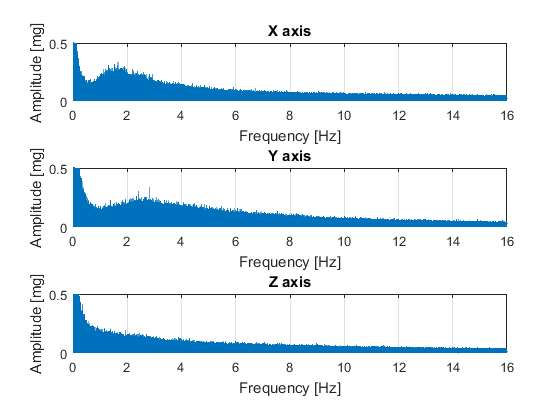
\includegraphics[width = 0.75\textwidth]{figures/frequencyanalysis2.png}
\caption{The results of the frequency analysis of the first data set. The frequency spectrum of each axis consists of significant components at frequencies close to zero-frequency and minor components at non-zero frequencies.} \label{frequenyspectrumfigure}
\end{figure}


\begin{figure}[h]
\centering
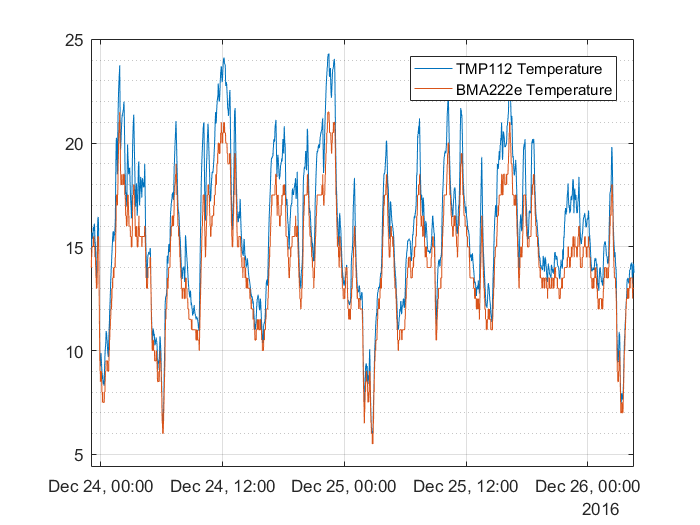
\includegraphics[width = 0.75\textwidth]{figures/lehma9885temperature.png}
\caption{The temperature sensor readings do not correlate with any other results. More likely, temperature correlates with the air temperature inside cowshed.} \label{cowtemperature}
\end{figure}





\subsubsection{SD File Operations}

In the first data recording process, it was desired to record the data in as high bandwidth as possible. The maximum bandwidth of the accelerometer were \SI{1000}{\hertz}. Consequently, the update time was \SI{0.5}{\milli \second}. However, the duration of SD file operations restricts the maximum recording bandwidth significantly. Finally, in the first data recording process the bandwidth was selected to be \SI{125}{\hertz}. Yet, the file operations exceeded the time \dots

SD card file operation times were recorded after the actual data recording using the original hardware. The original software was improved with timer operations in order to enable the recording of the file operation times. The file operation times had an affect on the data recording process. The time consumed for opening a file increased among the file size. The minimum opening time was \SI{7.26}{\milli\second} and the maximum time for \SI{1.37}{\giga \byte} file a was \SI{1440}{\milli \second}. The average value was \SI{747.14}{\milli \second}. The file closing times varied from \SI{8.04}{\milli \second} to \SI{160.03}{\milli \second} and seemed not to be dependent on the file size. The average file closing time was \SI{19.75}{\milli \second}. The time spent of writing a single data line was from \SI{56}{\micro \second} to \SI{162.36}{\milli\second} and the average was \SI{997.76}{\milli\second}. 



\begin{figure}[h]
\centering
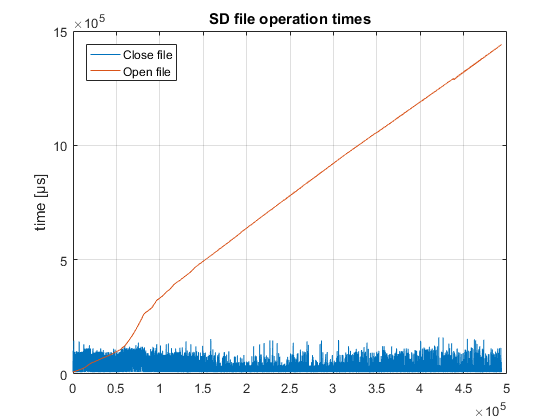
\includegraphics[width = 0.75\textwidth]{figures/openclosetimes_vanha.png}
\caption{} \label{openclosetimes_old}
\end{figure}

\begin{figure}[h]
\centering
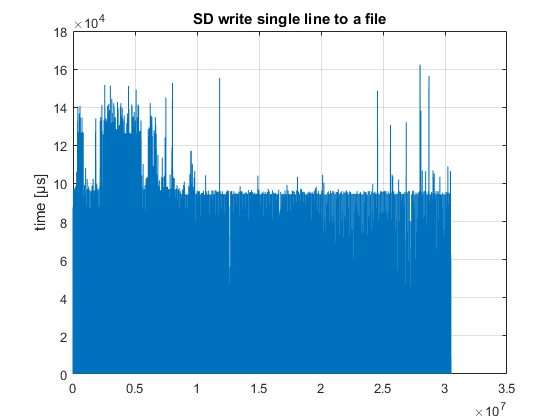
\includegraphics[width = 0.75\textwidth]{figures/writetimes_vanharauta.png}
\caption{} \label{writetimes_old}
\end{figure}


This subsection concentrates in the results of estrus detection. As discussed in section \ref{proceduresection} six cows were used in data recording process. However, two out of six data recordings failed. Thus, that data had to be discarded. The estruses were confirmed by Heatime estrus detection system. \\
In this study, a total of six cows were used for long period data recording.

\subsubsection{Behaviour monitoring}

\subsection{Algorithm Evaluation} \label{algorithmevaluationsection}

In previous subsection, we discussed of the results in general. The results of the first recorded data set were used for improving the sensor device application software as discussed in section \ref{softwaresection}. Conversely, the results of the second data set were used for developing and testing of the algorithms discussed in section \ref{estrusdetectionalgorithmssection}. An additional third set of data was further testing and tuning of the developed algorithms. In this section, we discuss of the results of the estrus detection algorithms. First we discuss of the results of estrus detection in general level. Additionally, we consider the affect of different parameters in estrus detection. Finally, we survey through each algorithm in separate subsections and discuss in detail of their pros and cons. \\
In order to validate the results of the algorithms, it is mandatory to define some measures of quality. Considering estrus detection, it is rather relevant to define if the cow is in estrus than how much it is in estrus. Therefore, simple categorization of the results such as positive and negative is a fair staring point. Additionally, the positive and negative results shall be divided into true and false results. In conclusion, we have four different measures for the results and they are defined as follows:


\begin{itemize}
\item \textit{True positive} means a condition when the algorithm detects an ongoing estrus and the cow is in estrus.
\item \textit{True Negative} is a condition when the estrus detection algorithm yields negative for estrus and the cow is not in estrus.
\item \textit{False positive} states that the estrus detection algorithm yields positive for estrus but the cow is not in estrus.
\item \textit{False negative} mean a condition when the estrus detection algorithm yields not in estrus but the cow is in estrus.
\end{itemize}

In addition to these measures, it is beneficial to be able to depict the differences between positive and negative periods. For example, comparison of the amplitudes. In the following subsections the results are normalized. That is, a median value is subtracted from all the data. Next the data is normalized so that, the extreme value is either $\pm1$. Therefore, we are able to compare the results within the algorithm as well as between the algorithms. 

In this study, the detected estruses are verified with Heatime estrus detection and rumination monitoring system. Thus, each cow wearing the sensor device of this study additionally dons Heatime sensor. The Heatime id considered relatively reliable in estrus detection. Nevertheless, none of the detected estruses were not veterinarian verified. Thus the results of this study are at most as reliable as the results of the Heatime. Furthermore, all the possible false detection of Heatime that conflicts with our device will remain unsolved in this study. \\
As discussed earlier, a total of six cows were used for the actual estrus data recording. The first three cows were 319, 659 and 9885 of which only two sets of data, 319 and 9885, were valid to use in the algorithm development. Both of the cows had two or more estruses in the data log of the Heatime as shown in pictures \ref{heatime_kiima_319} and \ref{heatime_kiima_9885}.The next three cows were 767, 787 and 812 of which only the data of 767 and 787 were valid to use in algorithm tuning and evaluation. Also both of these cows had detectable estruses in the log of Heatime. They are shown in pictures \ref{heatime_kiima_767} and \ref{heatime_kiima_787}. Nevertheless, the data recording period in this study lasted only approximately 30 days per instance. Thus, only one detectable estrus per cow were included in our recording period except the cow 9885 with two periods.




\begin{figure}[h]
\centering
\includegraphics[width = 0.75\textwidth]{figures/heatime_kiima_319}
\caption{The activity data of Heatime system of the cow 319. The cow has had estruses approximately on October the 30\textsuperscript{th} and December the 20\textsuperscript{th}. The latter of the estruses should be detectable in this study, hence it is within our data recording period.}
\label{heatime_kiima_319}
\end{figure}

\begin{figure}[h]
\centering
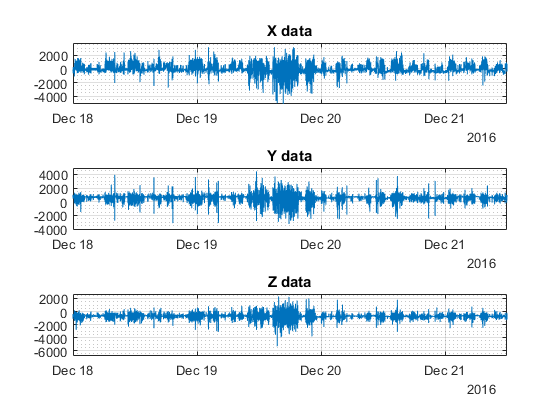
\includegraphics[width = 0.75\textwidth]{figures/kiimadata_319.png}
\caption{The raw acceleration data of each axis of the cow 319. The time frame of this picture is restricted around the estrus.}
\label{kiimadata_319}
\end{figure}



The proestrus period corresponding the detected estrus by Heatime is visually detectable in raw accelerometer data. The increased activity level of the cow appears in exceptionally long period of high amplitude activity. Furthermore, the change of activity is detectable in all axis of the accelerometer. Figure \ref{kiimadata_319} represents the raw accelerometer data of the cow 319 around of the proestrus period. Similarly, figures \ref{kiimadata_9885_1} and \ref{kiimadata_9885_2} shows the raw accelerometer data around the both proestrus periods of the cow 9885. In conclusion, these highly active periods are easily detectable for human simply by visually inspecting these plots. Nevertheless, it is necessary to develop computational algorithms that yields either\textit{is in estrus} or \textit{not in estrus}. However, it is the proestrus rather than the actual estrus. Thus, in algorithm level it is more sensible to define whether the cow is in proestrus or is not in proestrus. Consequently, the end of proestrus indicates the beginning of the estrus and this state transition shall be indicated to the end user.


The following subsections discuss of each estrus detection algorithm individually. First we start with the activity measurement algorithm, which is rather straight forwarding and does not require any advantageous computation. Second, we evaluate the variance detection algorithm which is based on variance of periodic short data samples. Lastly, we discuss of the inactivity detection algorithm, which detects rather lack of inactivity than activity directly. Additionally, we discuss of tuning of the algorithm parameters as well as the optimal results based on the recorder data. 

The parameters are tuned with iterative methods. That is, testing various values and evaluating the results before applying new values. This iteration is continued until, iteration yields no more benefits.


\begin{table} \caption{Increased activity periods detected with Heatime cow monitoring system. Increased activity is considered as proestrus. These detections are used as a reference in this study.}
\centering
\begin{tabular}{| p{1.25cm} | p{2.25cm} | p{9 cm} |}
\hline
\textbf{Cow ID} & \textbf{Occurrence of increased activity} & \textbf{Other notifications} \\  \hline
319 & 30-11-2016 & High activity period considered as pro-estrus. However, this period is outside of our sampling period. \\ \hline
319 & 19-12-2016 &  Second period of high activity considered as pro-estrus. This activity period is within our data recording period.  \\ \hline
9885 & 24-11-2016 & First high activity period of this cow and it is considered as a pro-estrus. However, the occurrence is outside of our data recording period.  \\ \hline
9885  & 22-12-2016  & The second activity period of this cow is considered as proestrus. However, this activity period is delayed possibly because of stress cause by the new sensor. Nevertheless, the proestrus is within our data recording period.  \\ \hline
9885  & 04-01-2017  & Third high activity period of the cow 9885. In contrast to the previous occurrence, this is slightly early. However, also this occurrence is within our data recording period.  \\ \hline
 767 &  21-01-2017 & The first high activity period of this cow. Unfortunately, the occurrence is outside of our data recording period.  \\ \hline
 767 & 13-02-2017  & The second activity period of this cow is within of our data recording period.  \\ \hline
 787 & 08-01-2017 &  The first activity period of this cow. However, the amplitude of the activity is not very high. Therefore, it is considered as proestrus with restrictions. Additionally, the occurrence is outside of our data recording period. \\ \hline
 787 & 19-01-2017  & The second increased activity period of the cow. This time the activity is high enough and the event should be considered as proestrus. However, also this occurrence is outside of our data recording period.  \\ \hline
 787 & 10-02-2017  &  The third occurrence of increased activity of this cow. The occurrence is within our data recording period. Thus it can be used as a reference in algorithm development. \\ \hline
\end{tabular}
\end{table}


\subsubsection{Activity Monitoring} \label{activitymeasurementevaluation}


\begin{figure}[htb]
\centering
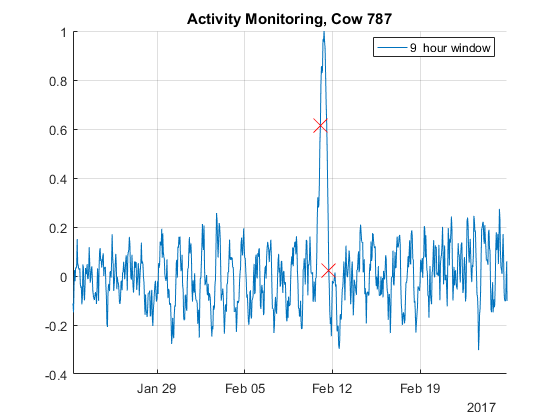
\includegraphics[width = 0.75 \textwidth]{figures/ActivityMonitoringCow787.png}
\caption{The results of activity measurement of the cow 787. The difference between the estrus and rest of the period is most distinct within this algorithm. Thus, the risk of false positive and false negative results is least significant.}
\label{ActivityMonitoringCow787}
\end{figure}

\begin{figure}[htb]
\centering
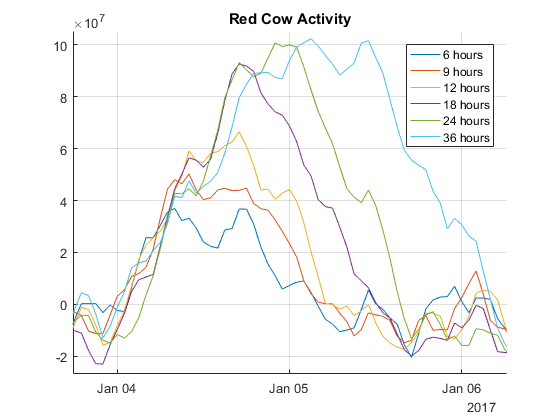
\includegraphics[width = 0.75\textwidth]{figures/redcowactivity2.png}
\caption{The activity plots of the second proestrus of the cow 9885. The figure illustrates the affect of varying the size of the integration window. Wider window increases the amplitude of the estrus and eases the detectability. However, simultaneously it delays the moment of detection. }
\label{integrationwindows}
\end{figure}



As stated earlier, data of four different cows were used in the algorithm development and data of two cows had to be discarded since it was not valid. Nevertheless, the data of four cows consists of five proestrus periods, and thus, slightly compensates the smaller amount of usable data.

The first estrus detection algorithm was based on activity measurement. In is very straight forwarding and does not require any complex computation. However, the algorithm is sensitive to offset in the data. Thus, the offset shall be removed with appropriate filter before integrating the values together. Developing of such filter requires knowledge of \dots

In despite of the complex algorithm development, the actual filtering requires simple floating point multiplications and summing depending of the order of the filter. Therefore, even with the offset compensating filter this algorithm is rather straight forward and mathematically simple. In contrast to its simplicity this algorithm requires continuous sampling and continuous computing of the samples. First, applying a high-pass filter as an offset compensation. Next, integrating the results. Additionally, there are only few tunable parameters that affect the estrus detection, width of the integration window and threshold. All the other parameters affect only to the computational load and visualization of the results.

According to the duration of proestrus, the optimal integration window is approximately from 9 to 12 hours. Narrower window might trigger the begin on estrus too early. Additionally, it makes the algorithm more sensitive to detect to false positives because the amplitude difference between proestrus and other periods decrease. Therefore, a scared cow behaving restlessly might yield false positive.

The results of the activity measurement algorithm are shown in figures \ref{ActivityMonitoringCow319}, \ref{ActivityMonitoringCow9885}, \ref{ActivityMonitoringCow767} and \ref{ActivityMonitoringCow787}. In these results, three different integration windows are included, 6 hour, 9 hours and 12 hours. In general, the performance of this algorithm is stable. No false positives of false negatives occurred. The difference between proestrus and other periods are obvious. However, the amplitude outside of proestrus is occasionally significant. In addition to the detected estruses, the affect of the width of the integration window is illustrated in picture \ref{integrationwindows}. It is seen that wider window delays the triggering of the end of the proestrus. Conversely, wider integration window enhances the amplitude of the proestrus phase. 

Quite straight-forward algorithm without any advantageous data processing. That is, the algorithm integrated the activity in certain periods and represented the activity of the period in one number. Required continuous sampling. Nevertheless, it detected all the estruses easily and no false positives were found.


\subsubsection{Variance Detection} \label{variancedetectionevaluation}

\begin{figure}[htb]
\centering
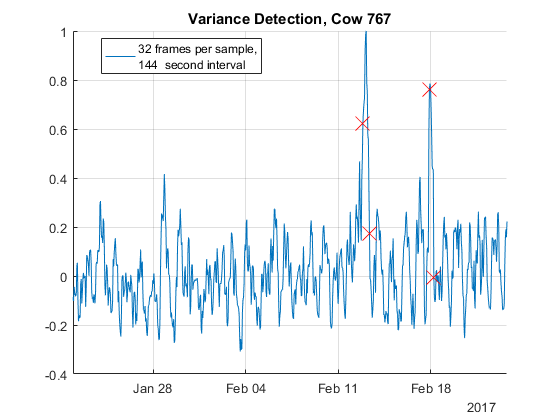
\includegraphics[width = 0.75 \textwidth]{figures/VarianceDetectionCow767_32frames144seconds.png}
\caption{More seldom sampling yield false positive results as seen in this picture.}
\label{VarianceDetectionCow767_32frames144seconds}
\end{figure}


Previously we discussed of activity measurement which is the most simple estrus detection algorithm of this study. It was based on continuous filtering and data sampling. Computationally, it was relatively simple but it loads the processor continuously. In contrast, the second estrus detection algorithm, variance detection, is based on samples with regular intervals instead of continuous data streams. Nevertheless, it is computationally slightly more complex than the former algorithm. However, it is still considered as suitable for micro-controller platforms. In addition to higher computational complexity of the algorithm, it comes with two additional tunable parameters, the size of the sample and sampling interval. In the optimized solution of this study, the sample size is 32 data frames and sampling interval is \SI{12}{\minute}. According to the configurations of the accelerometer, the 32 data frames responses to approximately 2 second period of data. 

Figures \ref{VarianceDetectionCow319}, \ref{VarianceDetectionCow9885}, \ref{VarianceDetectionCow767} and \ref{VarianceDetectionCow787} represents the results with optimized parameters. The parameters for all algorithms are common. As seen, the algorithms occationally detects the proestrus. However, the results includes numerous false positives and even one false negative with the cow 9885. The reliability, seems to depend on the cow and individually tuned parameters. Nevertheless, no appropriate parameters were found for all f the cows during this study.

The data of the cow 9885 were analyzed with various parameters because the algorithm yielded one true positive and one false negative. Thus it was interested to tune the parameters and see if the algorithm could yield two true positives.


Varying the sample size affect the results:







\subsubsection{Inactivity Detection}\label{inactivitydetectionevaluation}

\begin{figure}[htb]
\centering
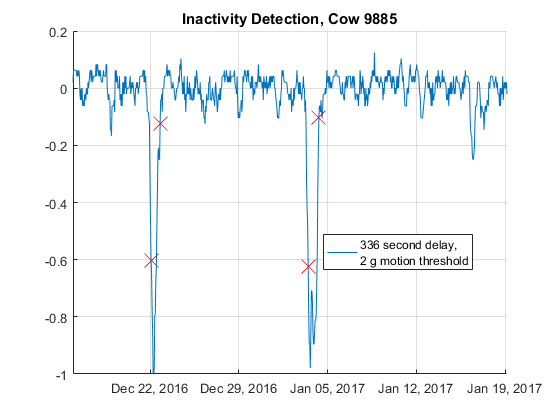
\includegraphics[width = 0.75 \textwidth]{figures/InactivityDetectionCow9885.png}
\caption{The results of inactivity detection algorithm of the cow 9885. The parameters are 336 second delay and \SI{2}{\gram} motion threshold. Both of the estruses are detected as true positive on December the 22\textsuperscript{nd} and January the 4\textsuperscript{th}. No false positive or false negative detection occurred. The amplitude difference between proestrus and non-estrus is obvious.}
\label{InactivityDetectionCow9885}
\end{figure}

Similarly to the variance detection algorithm, the inactivity detection algorithm has to more tunable parameters than the activity monitoring algorithm. Nevertheless, the parameters differ from the previous algorithms. That is, the tunable parameters are the motion threshold and the delay the motion shall not exceed the threshold. Otherwise, the algorithms follows similar integration time as the activity monitoring algorithm. Additionally, testing showed that this algorithm is not very sensitive to the parameters. Consequently, proestruses were detected as true positives with any feasible parameters. Furthermore, the algorithm did not yield any false positives or false negatives during this study.




The first set of data provided relatively wide frequency spectrum of data.


The sampling period provided a total of three probable estruses. One of the sensors failed during the sampling period, and therefore, no estrus could be estimated. However, one of the cows had two estruses during the sampling period and thus, compensated the failed sensor.

Based on pure visual analysis of the acceleration data, the red cow has two highly active proestrus periods. First begins December the 22nd at 9 pm end ends December the 23rd at 9 am. The second period begins January the 4th at 2 am and ends 6 pm. Proper insemination is from 6 to 24 hours after proestrus period.

The estrus was detected using Heatime estrus detection system. The detected estruses are represented in figures...



The activity could be measured in several ways. Pedometers measures the number of steps. However, sensor worn in neck could not probably be used for step counting and therefore, no steps were estimated. Human activity bracelets and other devices could measure steps but if total energy consumption is being estimated, the values of acceleration should be taken into account. A research have shown that the sum of absolute value of the axis, instead of a absolute value is the best simple estimate for energy consumption and therefore, a good activity measure.

The cow activity was measured as a sum of absolute value acceleration vector. The activity was summed over a varying time window from 6 hours to 36 six hours. Since the resulting activity is always a sum of past activity, this method causes delay and widening of the activity peak. However, the size of the window does not affect the steepness of the rising or falling edges. Nevertheless, the size of the window widens the peaks if the window size is too high. In result, increasing the window might delay the estrus detection, if the detection has dependencies in the falling edge. Based on the three found heat activity peaks of estrus, an optimal window size is somewhere between 9 end 12 hours.



\subsection{Conclusions} \label{conclusionssection}

Previously in this section we discussed of the results of the research of this study. First, we discussed the results in general level. Next we focused on presenting the results of the estrus detection algorithms. Consequently, in this subsection we will draw conclusions based on the presented results. First, we will evaluate sensor based estrus detection as a concept. The evaluation will take into account former studies as well as the results gained in this study. Second, We will focus on failures of this study and propose actions to correct the failures and mistakes. Third, the scope is in suggestions for the future studies as continuation for this study.

\subsubsection{Sensor Based Estrus Detection}

This study introduced a sensor device for dairy cow estrus detection. The introduction included as well as the hardware configuration as well as the software implementation. Furthermore, we discussed of three different estrus detection algorithms suitable for the device. Practically, the algorithms were developed and tested with Matlab on computer after recording of real cow data. The algorithms were different in their approach to the topic. However, all of them were based on the accelerometer data only. In general, all of the algorithms performed the estrus detection well after tuning of the algorithm specific parameters. Nevertheless, there were differences in the reliability as well as in the clearance of the results. The conclusions of the algorithms are discussed in following.

The activity monitoring algorithm was a straightforward integration of the accelerometer data. The only tunable parameter was the size of the integration time. The most suitable integration time corresponds approximately the duration of the proestrus phase of the estrus cycle, that is roughly from 9 to \SI{12}{\hour}. Extending of the integration time only delayed the triggering of the begin of estrus. Thus, it was not beneficial. Conversely, integration time less than \SI{6}{\hour} yielded a risk of triggering estrus too early in the middle of the proestrus phase. These results were so obvious, hence, it was decided to use \SI{9}{\hour} window with the rest of the algorithms without further tuning of it. Furthermore, the algorithm was quite robust. That is, the results were clear and there were no high risk of yielding false results within the suggested integration time. However, the algorithm is sensitive to data offset and it shall be removed before any other computation. Nevertheless, offset did not prevent from detecting the estrus in this study. Actually, it only reduced the amplitude difference between the proestrus and other periods.

In contrast to the activity monitoring algorithm, the variance detection algorithm was sensitive to the parameters. That is, too short sample or too long sampling interval effected to the results significantly. However, \dots

Similarly to the variance detection, the inactivity detection algorithm had two additional tunable parameters. However, inactivity detection did not seem to be sensitive to the tuning of the parameters. In this study, any reasonable parameter values yielded true positive and true negative results. Furthermore, no false results occurred. Nevertheless,  the most radical parameter values begun to affect to the amplitude difference between proestrus and other phases of the estrus cycle. In conclusion, the performance and reliability of this algorithm seemed most promising in this study. Furthermore, this algorithm is the most suitable for the micro-controller based solutions. That is, most of the computations are performed in the accelerometer and the micro-controller only summarizes seldom interrupt the accelerometer generates. Additionally, it enables efficient use of power saving modes of the micro-controller which is critical with battery powered solutions. 


The dairy cow estrus is detectable with triaxial accelerometer only and no other sensors are required. The results were verified with one single commercial product. Thus, the results may not be completely reliable and valid. Furthermore, none of the detected estruses were verified by a vet.

The estrus detection algorithms developed in this study are suitable for micro-controller environments. Therefore, algorithm computation with computers is not required. Consequently, there is no need to large data storage or transmitting raw sensor data wirelessly.


\subsubsection{Failures and considerations}

Previously, we discussed of sensor based dairy cow estrus detection based on the results of this study. The conclusion was that the estrus of a dairy cow is detectable with an accelerometer base wearable sensor. Furthermore, it seemed the estrus is rather detectable with various algorithms. However, there were differences in the performance and reliability of different algorithms. Whereas the previous subsection focused on the successful part of this study, in this subsection the scope is in failures and suggestions for improvements.

Firstly, the body temperature measurement was a total failure. That is, the heat conducting system did not conduct the heat enough. Conversely, the results of the temperature measurements seemed to follow the temperature of the surrounding air. It was also seen from the temperature curve of the accelerometer \ref{cowtemperature}, hence, both of the temperatures seemed synchronous. Additionally, it was tested to filter the results and calculate the differential of the two temperatures sensors. Nevertheless, no correlation with a ongoing estrus or proestrus were found in this study. In contrast to the sensor setup of this study, the temperature sensor should be placed into more direct skin contact. Thereby, the sensor would more likely measure the body temperature rather than the surrounding air. Nevertheless, this discussion is only hypothetical. Furthermore, the body temperature was assumed to rise only up to two degrees during the estrus. Therefore, detecting of such minor alterations with micro-controller suitable algorithms may not be reliable at all.

Secondly, total of three attempts to record cow data were ruined because of an error state of the sensor device. Unfortunately, there was no method to define the cause of the error directly. However, it seemed that the device continued working even in the error state but the data was invalid. However, further analysis of the error data provided an assumption that the accelerometer had reset meanwhile the micro-controller had not. Consequently, the micro-controller stopped receiving any interrupts from the accelerometer. Furthermore, the range of the accelerometer was set to default of \SI{2}{\gram}. Meanwhile, the micro-controller applications continued of executing of its software loop. Nevertheless, without fetching data normally. Therefore in both software implementations, the watchdog timer triggered an event for reading single data frame from the FIFO memory of the accelerometer. Considering the number of the invalid samples and the period of watchdog timer matched with the time cow was wearing the sensor. In order to avoid such failures in the future, the software should include a method for detecting erroneous state of the accelerometer. Additionally, the hardware might be causing blackouts to the accelerometer. This possibility should be inspected and the hardware design improved according the discoveries.

Lastly, the hardware design did not provide optimal performance for high sampling rate as seen in section \ref{generalresultssection}. Therefore, the first recorded set of data was partially corrupted because of frequent buffer overflows. Furthermore, high sampling rate fulfilled the SD memory card relatively fast. Thus high sampling rate together with SD memory card would not be preferred solution in long term data recording. 



\subsubsection{Suggestions for Future Studies}

This study has introduced three different sensor based algorithms for dairy cow estrus detection. Furthermore, we have evaluated the algorithms and concluded that the estrus id detectable with accelerometer based wearable sensor. Additionally, we have discussed of secondary products and other observations during this study. Lastly in this study, we will discuss of suggestions for potential future studies based on the introduced results and conclusions.

Firstly, the detected estruses in this study were not confirmed at any point. The results were verified only with another sensor device as a reference. Thus, the results of this study are not completely reliable. Therefore, the algorithms developed in this study shall be implemented directly for micro-controller. Furthermore, they shall be tested with dairy cattle in real-time instead of posterior data processing sessions. In order to fully validate the algorithms, the results shall be verified by a veterinary. That is, each cow shall be inseminated once an estrus has been detected. Consequently, the detection is considered as true positive if the insemination is successful and the cow becomes pregnant.  Nevertheless, the normal success rate of insemination as well as the estrus cycle shall be taken into account.

Secondly, the amount of data used for algorithm development was quite small. That is, only four months of cow data was valid to use in algorithm development. Luckily, the data consisted total of five estruses. Nevertheless, statistically sampling is minor considering the head count world wide. Furthermore, it is assumed there are significant differences in cow activity levels, hence, it varied already in this study. Additionally, a complementary study should cover various breeds in various environments e.g., tie-stall and pasture. Furthermore, we did no discuss of  algorithm tuning thoughtfully. Actually, the methods of this study tuned the algorithms for each cow individually after analyzing all of the data. Thus, the parameters suitable for one cow might not be suitable for another. However, more of recorded data would enable the developing of algorithms with self-adjustable parameters. Consequently, it would improve the real-time performance of the estrus detection algorithms discussed in this study.

Thirdly, behavior monitoring was considered as on optional topic in this study. A successful behavior monitoring would provide prominent information for the farmer about the state of the cattle. Furthermore, exceptions in behavior could indicate concerns in the cows health and treatment could be started before issues escalate. In this study, we recorded in-cowshed video for studying of behavior recognition. However, the the video quality was insufficient and there were no valid time synchronization between the video and motion data. Thus, this option was discarded in early phase of this study. However, based on the brief preliminary study, this option seemed promising. Therefore, study of valid motion and video data with proper time synchronization would provide algorithms for such topics as rumination and lameness detection.


\clearpage

\section{Summary} \label{summarysection}


Summary of all the previous. Alternatively ``Discussion'' or ``Conclusions''...


\clearpage
%% Lähdeluettelo

\thesisbibliography

%\begin{thebibliography}{99}

\begin{thebibliography}{99}

\begin{thebibliography}{99}

\include{bibliography.tex}

%% Alla pilkun jälkeen on pakotettu oikea väli \<välilyönti>-merkeillä.
\bibitem{Kauranen} Kauranen,\ I., Mustakallio,\ M. ja Palmgren,\ V.
  \textit{Tutkimusraportin kirjoittamisen opas opinnäytetyön
    tekijöille.}  Espoo, Teknillinen korkeakoulu, 2006.

\bibitem{Itkonen} Itkonen,\ M. \textit{Typografian käsikirja.} 3.\
  painos.  Helsinki, RPS-yhtiöt, 2007.

\bibitem{Koblitz} Koblitz,\ N. \textit{A Course in Number Theory and
    Cryptography. Graduate Texts in Mathematics 114.}  2.\ painos. New
  York, Springer, 1994.

%% Kun on useampi nimikirjain, jokaisen nimikirjaimen väliin
%% kuuluu välilyönti. Oikea välin määrä on saatu \<välilyönnillä>
\bibitem{bcs} Bardeen,\ J., Cooper,\ L.\ N. ja Schrieffer,\ J.\ R.
  Theory of Superconductivity. \textit{Physical Review,} 1957, vol.\
  108, nro~5, s.\ 1175--1204.

\bibitem{Deschamps} Deschamps,\ G.\ A. Electromagnetics and
  Differential Forms. \textit{Proceedings of the IEEE,} 1981, vol.\
  69, nro~6, s.\ 676--696.

%% Alla esimerkki englanninkielisen tavuttamisen pakottamisesta.
%% Oletusarvoisesti käytetään suomalaista tavutusta, mutta viitteissä
%% esiintyy usein muunkielisiä lauseita, jotka tulevat siten tavutetuksi
%% suomen kielen sääntöjen mukaan. Tämän voi korjata \foreignlanguage-
%% komennolla, jonka ensimmäinen parametri on vieraan kielen nimi ja toinen 
%% on vieraalla kielellä tavutettava teksti. 
\bibitem{Sihvola} Sihvola,\ A.\ et al.
  \foreignlanguage{english}{Interpretation of measurements of helix 
    and bihelix superchiral structures.}
  Teoksessa: Jacob,\ A.\ F. ja
  Reinert,\ J. (toim.) \textit{Bianisotropics '98 7th International
    Conference on Complex Media.}  Braunschweig, 3.--6.6.1998.
  Braunscweig, Technische Universität Braunschweig, 1998, s.\
  317--320.

%% Alla on suomalainen yhdistelmäsukunimi. Sen nimien välissä 
%% käytetään yhdysmerkkiä l. tavuviivaa, kirjoitetaan -.
\bibitem{Lindblom} Lindblom-Ylänne,\ S. ja Wager,\ M.  Tieteellisten
  opinnäytetöiden ohjaaminen. Teoksessa: Lindblom-Ylänne,\ S. ja
  Nevgi,\ A. (toim.) \textit{Yliopisto- ja korkeakouluopettajan
    käsikirja.}  Helsinki, WSOY, 2004, s.\ 314--325.
 
\bibitem{Miinusmaa} Miinusmaa,\ H. Neliskulmaisen reiän poraamisesta
  kolmikulmaisella poralla. Diplomityö, Teknillinen korkeakoulu,
  konetekniikan osasto, Espoo, 1977.

%% Tässä taas pakotettu englanninkielinen tavutus. 
%% Pedanttinen kirjoittaja pakottaa tietysti jokaiseen englanninkieliseen
%% lauseeseen englannin tavutuksen, mutta tässä esityksessä ei näin ole
%% tehty selvyyden ja lähdekoodin luettavuuden takia. 
\bibitem{Loh} Loh,\ N.\ C. High-Resolution Micromachined
  Interferometric Accelerometer. Master's Thesis, Massachusetts
  Institute of Technology, Cambridge,
  \foreignlanguage{english}{Massachusetts,} 1992.

\bibitem{Lonnqvist} Lönnqvist,\ A.
  \foreignlanguage{english}{Applications of hologram-based compact
    range: antenna radiation pattern, radar cross section, and
    absorber reflectivity measurements.}
  Väitöskirja, Teknillinen korkeakoulu, sähkö- ja tietoliikennetekniikan
  osasto, 2006.

\bibitem{sfs} SFS 5342. Kirjallisuusviitteiden laatiminen. 2.\ painos.
  Helsinki, Suomen standardisoimisliitto, 2004. 20~s.

\bibitem{haastattelu} Palmgren,\ V. Suunnittelija. Teknillinen
  korkeakoulu, kirjasto. Otaniementie 9, 02150 Espoo. Haastattelu
  15.1.2007.

\bibitem{Ribeiro} Ribeiro,\ C.\ B., Ollila,\ E. ja Koivunen,\ V.
  \foreignlanguage{english}{Stochastic Maximum-Likelihood Method for
    MIMO Propagation Parameter Estimation.}
 \textit{IEEE Transactions
    on Signal Processing,} verkkolehti, vol.\ 55, nro~1, s.\ 46--55.
  Viitattu 19.1.2007. Lehti ilmestyy myös painettuna. DOI:
  10.1109/TSP.2006.882057.

\bibitem{Stieber} Stieber,\ T. GnuPG Hacks. \textit{Linux Journal,}
  verkkolehti, 2006, maaliskuu, nro~143. Viitattu 19.1.2007. Lehti
  ilmestyy myös painettuna. Saatavissa:
  \url{http://www.linuxjournal.com/article/8732.}

\bibitem{kone} Pohjois-Koivisto,\ T. Voiko kone tulevaisuudessa arvata
  tahtosi?  \textit{Apropos,} verkkolehti, helmikuu, nro~1, 2005.
  Viitattu 19.1.2007.  Saatavissa:
  \url{http://www.apropos.fi/1-2005/prima.php.}

\bibitem{Adida} Adida,\ B.  Advances in Cryptographic Voting Systems.
  Verkkodokumentti. Ph.D.\ Thesis, Massachusetts Institute of
  Technology, Cambridge, 
  \foreignlanguage{english}{Massachusetts,}
  2006. Viitattu 19.1.2007.  Saatavissa:
  \url{http://crypto.csail.mit.edu/~cis/theses/adida-phd.pdf.}

\bibitem{viittaaminen} Kilpeläinen,\ P. WWW-lähteisiin viittaaminen
  tutkielmatekstissä. Verkkodokumentti. Päivitetty 26.11.2001.
  Viitattu 19.1.2007. Saatavissa:
  \url{http://www.cs.uku.fi/~kilpelai/wwwlahteet.html.}

\end{thebibliography}

%% Alla pilkun jälkeen on pakotettu oikea väli \<välilyönti>-merkeillä.
\bibitem{Kauranen} Kauranen,\ I., Mustakallio,\ M. ja Palmgren,\ V.
  \textit{Tutkimusraportin kirjoittamisen opas opinnäytetyön
    tekijöille.}  Espoo, Teknillinen korkeakoulu, 2006.

\bibitem{Itkonen} Itkonen,\ M. \textit{Typografian käsikirja.} 3.\
  painos.  Helsinki, RPS-yhtiöt, 2007.

\bibitem{Koblitz} Koblitz,\ N. \textit{A Course in Number Theory and
    Cryptography. Graduate Texts in Mathematics 114.}  2.\ painos. New
  York, Springer, 1994.

%% Kun on useampi nimikirjain, jokaisen nimikirjaimen väliin
%% kuuluu välilyönti. Oikea välin määrä on saatu \<välilyönnillä>
\bibitem{bcs} Bardeen,\ J., Cooper,\ L.\ N. ja Schrieffer,\ J.\ R.
  Theory of Superconductivity. \textit{Physical Review,} 1957, vol.\
  108, nro~5, s.\ 1175--1204.

\bibitem{Deschamps} Deschamps,\ G.\ A. Electromagnetics and
  Differential Forms. \textit{Proceedings of the IEEE,} 1981, vol.\
  69, nro~6, s.\ 676--696.

%% Alla esimerkki englanninkielisen tavuttamisen pakottamisesta.
%% Oletusarvoisesti käytetään suomalaista tavutusta, mutta viitteissä
%% esiintyy usein muunkielisiä lauseita, jotka tulevat siten tavutetuksi
%% suomen kielen sääntöjen mukaan. Tämän voi korjata \foreignlanguage-
%% komennolla, jonka ensimmäinen parametri on vieraan kielen nimi ja toinen 
%% on vieraalla kielellä tavutettava teksti. 
\bibitem{Sihvola} Sihvola,\ A.\ et al.
  \foreignlanguage{english}{Interpretation of measurements of helix 
    and bihelix superchiral structures.}
  Teoksessa: Jacob,\ A.\ F. ja
  Reinert,\ J. (toim.) \textit{Bianisotropics '98 7th International
    Conference on Complex Media.}  Braunschweig, 3.--6.6.1998.
  Braunscweig, Technische Universität Braunschweig, 1998, s.\
  317--320.

%% Alla on suomalainen yhdistelmäsukunimi. Sen nimien välissä 
%% käytetään yhdysmerkkiä l. tavuviivaa, kirjoitetaan -.
\bibitem{Lindblom} Lindblom-Ylänne,\ S. ja Wager,\ M.  Tieteellisten
  opinnäytetöiden ohjaaminen. Teoksessa: Lindblom-Ylänne,\ S. ja
  Nevgi,\ A. (toim.) \textit{Yliopisto- ja korkeakouluopettajan
    käsikirja.}  Helsinki, WSOY, 2004, s.\ 314--325.
 
\bibitem{Miinusmaa} Miinusmaa,\ H. Neliskulmaisen reiän poraamisesta
  kolmikulmaisella poralla. Diplomityö, Teknillinen korkeakoulu,
  konetekniikan osasto, Espoo, 1977.

%% Tässä taas pakotettu englanninkielinen tavutus. 
%% Pedanttinen kirjoittaja pakottaa tietysti jokaiseen englanninkieliseen
%% lauseeseen englannin tavutuksen, mutta tässä esityksessä ei näin ole
%% tehty selvyyden ja lähdekoodin luettavuuden takia. 
\bibitem{Loh} Loh,\ N.\ C. High-Resolution Micromachined
  Interferometric Accelerometer. Master's Thesis, Massachusetts
  Institute of Technology, Cambridge,
  \foreignlanguage{english}{Massachusetts,} 1992.

\bibitem{Lonnqvist} Lönnqvist,\ A.
  \foreignlanguage{english}{Applications of hologram-based compact
    range: antenna radiation pattern, radar cross section, and
    absorber reflectivity measurements.}
  Väitöskirja, Teknillinen korkeakoulu, sähkö- ja tietoliikennetekniikan
  osasto, 2006.

\bibitem{sfs} SFS 5342. Kirjallisuusviitteiden laatiminen. 2.\ painos.
  Helsinki, Suomen standardisoimisliitto, 2004. 20~s.

\bibitem{haastattelu} Palmgren,\ V. Suunnittelija. Teknillinen
  korkeakoulu, kirjasto. Otaniementie 9, 02150 Espoo. Haastattelu
  15.1.2007.

\bibitem{Ribeiro} Ribeiro,\ C.\ B., Ollila,\ E. ja Koivunen,\ V.
  \foreignlanguage{english}{Stochastic Maximum-Likelihood Method for
    MIMO Propagation Parameter Estimation.}
 \textit{IEEE Transactions
    on Signal Processing,} verkkolehti, vol.\ 55, nro~1, s.\ 46--55.
  Viitattu 19.1.2007. Lehti ilmestyy myös painettuna. DOI:
  10.1109/TSP.2006.882057.

\bibitem{Stieber} Stieber,\ T. GnuPG Hacks. \textit{Linux Journal,}
  verkkolehti, 2006, maaliskuu, nro~143. Viitattu 19.1.2007. Lehti
  ilmestyy myös painettuna. Saatavissa:
  \url{http://www.linuxjournal.com/article/8732.}

\bibitem{kone} Pohjois-Koivisto,\ T. Voiko kone tulevaisuudessa arvata
  tahtosi?  \textit{Apropos,} verkkolehti, helmikuu, nro~1, 2005.
  Viitattu 19.1.2007.  Saatavissa:
  \url{http://www.apropos.fi/1-2005/prima.php.}

\bibitem{Adida} Adida,\ B.  Advances in Cryptographic Voting Systems.
  Verkkodokumentti. Ph.D.\ Thesis, Massachusetts Institute of
  Technology, Cambridge, 
  \foreignlanguage{english}{Massachusetts,}
  2006. Viitattu 19.1.2007.  Saatavissa:
  \url{http://crypto.csail.mit.edu/~cis/theses/adida-phd.pdf.}

\bibitem{viittaaminen} Kilpeläinen,\ P. WWW-lähteisiin viittaaminen
  tutkielmatekstissä. Verkkodokumentti. Päivitetty 26.11.2001.
  Viitattu 19.1.2007. Saatavissa:
  \url{http://www.cs.uku.fi/~kilpelai/wwwlahteet.html.}

\end{thebibliography}

%% Alla pilkun jälkeen on pakotettu oikea väli \<välilyönti>-merkeillä.
\bibitem{Kauranen} Kauranen,\ I., Mustakallio,\ M. ja Palmgren,\ V.
  \textit{Tutkimusraportin kirjoittamisen opas opinnäytetyön
    tekijöille.}  Espoo, Teknillinen korkeakoulu, 2006.

\bibitem{Itkonen} Itkonen,\ M. \textit{Typografian käsikirja.} 3.\
  painos.  Helsinki, RPS-yhtiöt, 2007.

\bibitem{Koblitz} Koblitz,\ N. \textit{A Course in Number Theory and
    Cryptography. Graduate Texts in Mathematics 114.}  2.\ painos. New
  York, Springer, 1994.

%% Kun on useampi nimikirjain, jokaisen nimikirjaimen väliin
%% kuuluu välilyönti. Oikea välin määrä on saatu \<välilyönnillä>
\bibitem{bcs} Bardeen,\ J., Cooper,\ L.\ N. ja Schrieffer,\ J.\ R.
  Theory of Superconductivity. \textit{Physical Review,} 1957, vol.\
  108, nro~5, s.\ 1175--1204.

\bibitem{Deschamps} Deschamps,\ G.\ A. Electromagnetics and
  Differential Forms. \textit{Proceedings of the IEEE,} 1981, vol.\
  69, nro~6, s.\ 676--696.

%% Alla esimerkki englanninkielisen tavuttamisen pakottamisesta.
%% Oletusarvoisesti käytetään suomalaista tavutusta, mutta viitteissä
%% esiintyy usein muunkielisiä lauseita, jotka tulevat siten tavutetuksi
%% suomen kielen sääntöjen mukaan. Tämän voi korjata \foreignlanguage-
%% komennolla, jonka ensimmäinen parametri on vieraan kielen nimi ja toinen 
%% on vieraalla kielellä tavutettava teksti. 
\bibitem{Sihvola} Sihvola,\ A.\ et al.
  \foreignlanguage{english}{Interpretation of measurements of helix 
    and bihelix superchiral structures.}
  Teoksessa: Jacob,\ A.\ F. ja
  Reinert,\ J. (toim.) \textit{Bianisotropics '98 7th International
    Conference on Complex Media.}  Braunschweig, 3.--6.6.1998.
  Braunscweig, Technische Universität Braunschweig, 1998, s.\
  317--320.

%% Alla on suomalainen yhdistelmäsukunimi. Sen nimien välissä 
%% käytetään yhdysmerkkiä l. tavuviivaa, kirjoitetaan -.
\bibitem{Lindblom} Lindblom-Ylänne,\ S. ja Wager,\ M.  Tieteellisten
  opinnäytetöiden ohjaaminen. Teoksessa: Lindblom-Ylänne,\ S. ja
  Nevgi,\ A. (toim.) \textit{Yliopisto- ja korkeakouluopettajan
    käsikirja.}  Helsinki, WSOY, 2004, s.\ 314--325.
 
\bibitem{Miinusmaa} Miinusmaa,\ H. Neliskulmaisen reiän poraamisesta
  kolmikulmaisella poralla. Diplomityö, Teknillinen korkeakoulu,
  konetekniikan osasto, Espoo, 1977.

%% Tässä taas pakotettu englanninkielinen tavutus. 
%% Pedanttinen kirjoittaja pakottaa tietysti jokaiseen englanninkieliseen
%% lauseeseen englannin tavutuksen, mutta tässä esityksessä ei näin ole
%% tehty selvyyden ja lähdekoodin luettavuuden takia. 
\bibitem{Loh} Loh,\ N.\ C. High-Resolution Micromachined
  Interferometric Accelerometer. Master's Thesis, Massachusetts
  Institute of Technology, Cambridge,
  \foreignlanguage{english}{Massachusetts,} 1992.

\bibitem{Lonnqvist} Lönnqvist,\ A.
  \foreignlanguage{english}{Applications of hologram-based compact
    range: antenna radiation pattern, radar cross section, and
    absorber reflectivity measurements.}
  Väitöskirja, Teknillinen korkeakoulu, sähkö- ja tietoliikennetekniikan
  osasto, 2006.

\bibitem{sfs} SFS 5342. Kirjallisuusviitteiden laatiminen. 2.\ painos.
  Helsinki, Suomen standardisoimisliitto, 2004. 20~s.

\bibitem{haastattelu} Palmgren,\ V. Suunnittelija. Teknillinen
  korkeakoulu, kirjasto. Otaniementie 9, 02150 Espoo. Haastattelu
  15.1.2007.

\bibitem{Ribeiro} Ribeiro,\ C.\ B., Ollila,\ E. ja Koivunen,\ V.
  \foreignlanguage{english}{Stochastic Maximum-Likelihood Method for
    MIMO Propagation Parameter Estimation.}
 \textit{IEEE Transactions
    on Signal Processing,} verkkolehti, vol.\ 55, nro~1, s.\ 46--55.
  Viitattu 19.1.2007. Lehti ilmestyy myös painettuna. DOI:
  10.1109/TSP.2006.882057.

\bibitem{Stieber} Stieber,\ T. GnuPG Hacks. \textit{Linux Journal,}
  verkkolehti, 2006, maaliskuu, nro~143. Viitattu 19.1.2007. Lehti
  ilmestyy myös painettuna. Saatavissa:
  \url{http://www.linuxjournal.com/article/8732.}

\bibitem{kone} Pohjois-Koivisto,\ T. Voiko kone tulevaisuudessa arvata
  tahtosi?  \textit{Apropos,} verkkolehti, helmikuu, nro~1, 2005.
  Viitattu 19.1.2007.  Saatavissa:
  \url{http://www.apropos.fi/1-2005/prima.php.}

\bibitem{Adida} Adida,\ B.  Advances in Cryptographic Voting Systems.
  Verkkodokumentti. Ph.D.\ Thesis, Massachusetts Institute of
  Technology, Cambridge, 
  \foreignlanguage{english}{Massachusetts,}
  2006. Viitattu 19.1.2007.  Saatavissa:
  \url{http://crypto.csail.mit.edu/~cis/theses/adida-phd.pdf.}

\bibitem{viittaaminen} Kilpeläinen,\ P. WWW-lähteisiin viittaaminen
  tutkielmatekstissä. Verkkodokumentti. Päivitetty 26.11.2001.
  Viitattu 19.1.2007. Saatavissa:
  \url{http://www.cs.uku.fi/~kilpelai/wwwlahteet.html.}

\end{thebibliography}



\printbibliography




%% Liitteet
\clearpage

\thesisappendix

%\clearpage
\section{Heatime Data Plots}

\begin{figure}[h]
\centering
\includegraphics[width = 0.75\textwidth]{figures/heatime_kiima_319}
\caption{The activity data of Heatime system of the cow 319. The cow has had estruses approximately on October the 30\textsuperscript{th} and December the 20\textsuperscript{th}. The latter of the estruses should be detectable in this study, hence it is within our data recording period.}
\label{heatime_kiima_319}
\end{figure}


\begin{figure}[h]
\centering
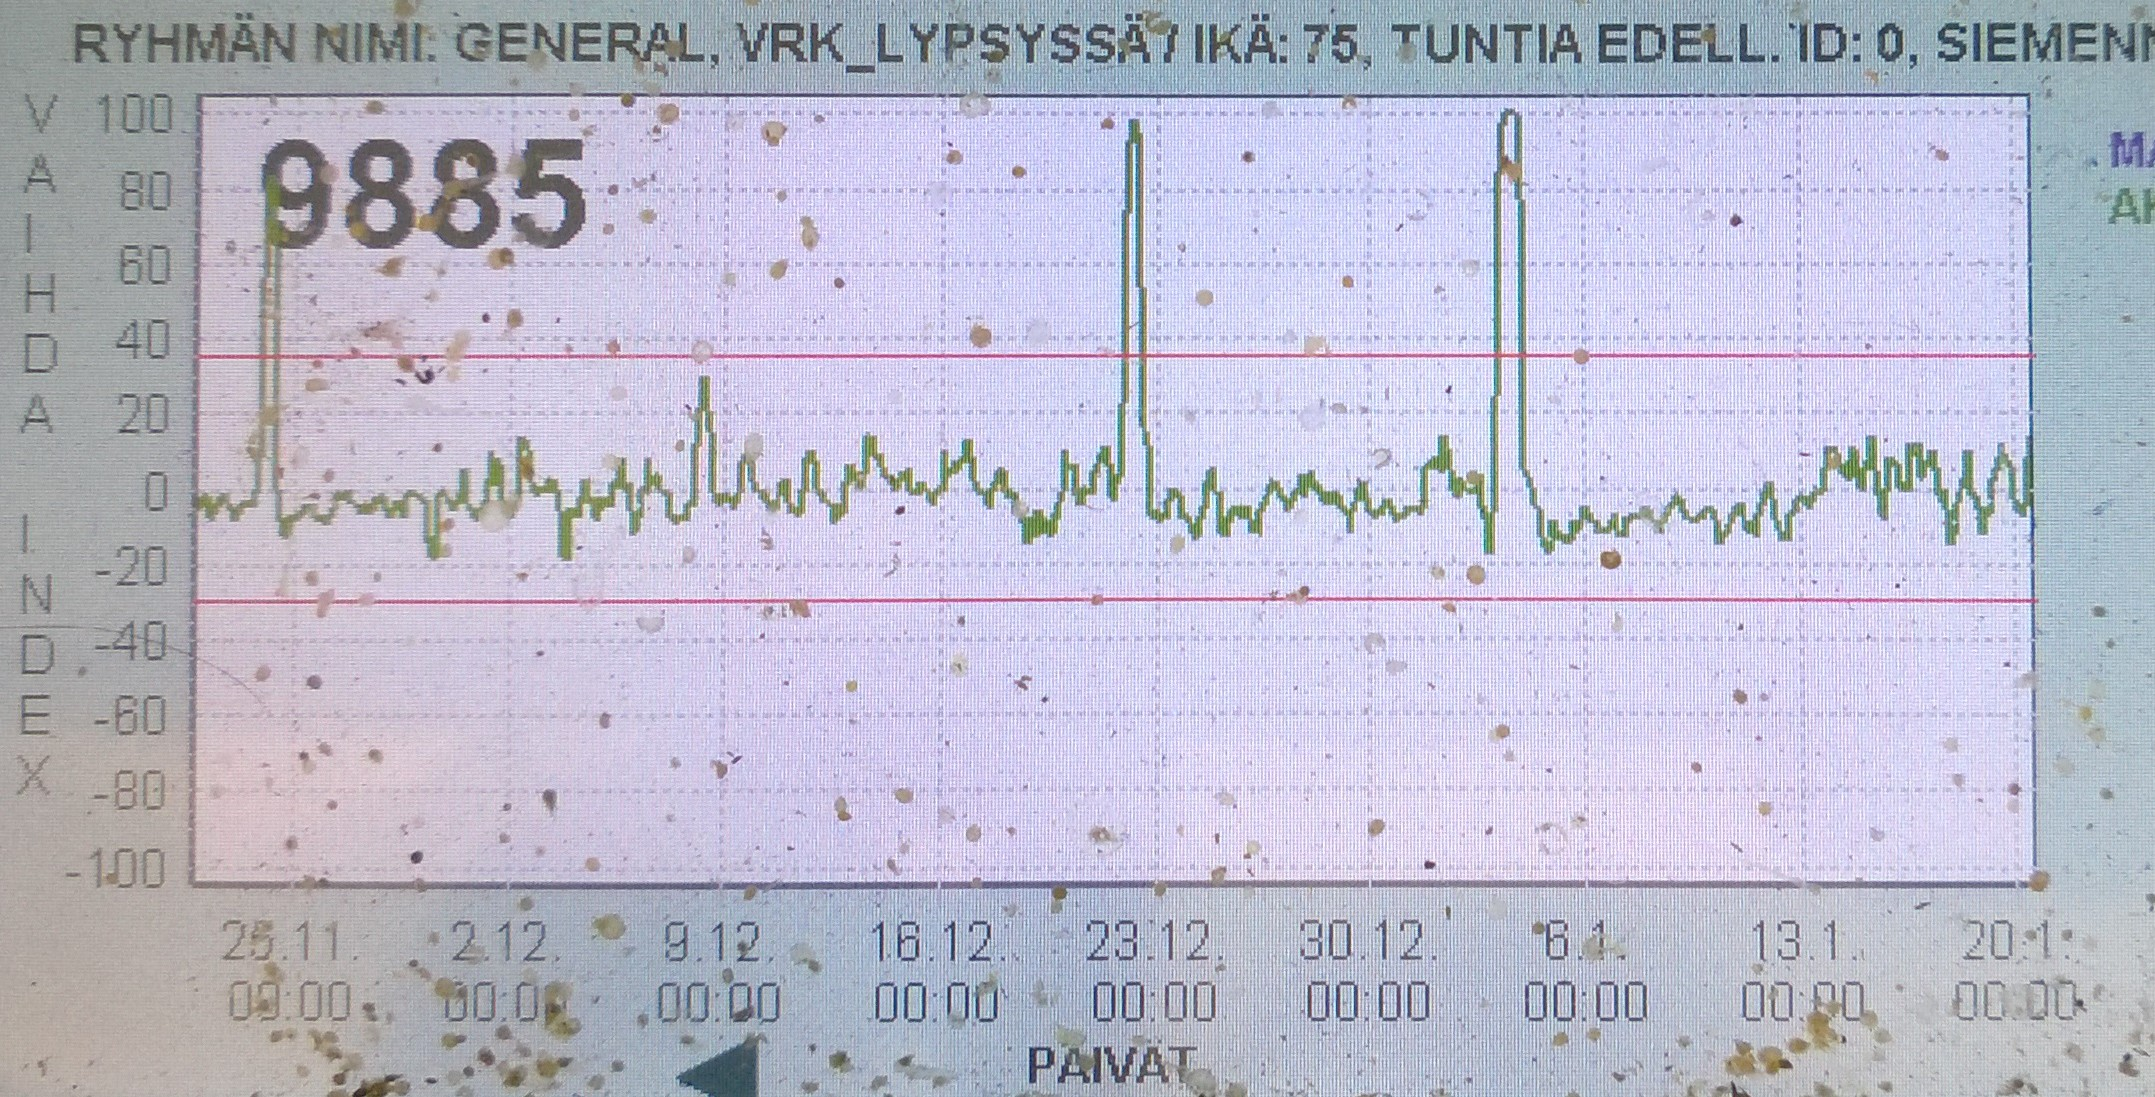
\includegraphics[width = 0.75\textwidth]{figures/heatime_kiima_9885}
\caption{The activity data of Heatime system of the cow 9885. The cow has had estruses approximately on October the 24\textsuperscript{th}, December the 22\textsuperscript{nd} and January the 4\textsuperscript{th}. Two latter estruses should be detectable in this study, hence they both are within our dat recording period. }
\label{heatime_kiima_9885}
\end{figure}

\begin{figure}[h]
\centering
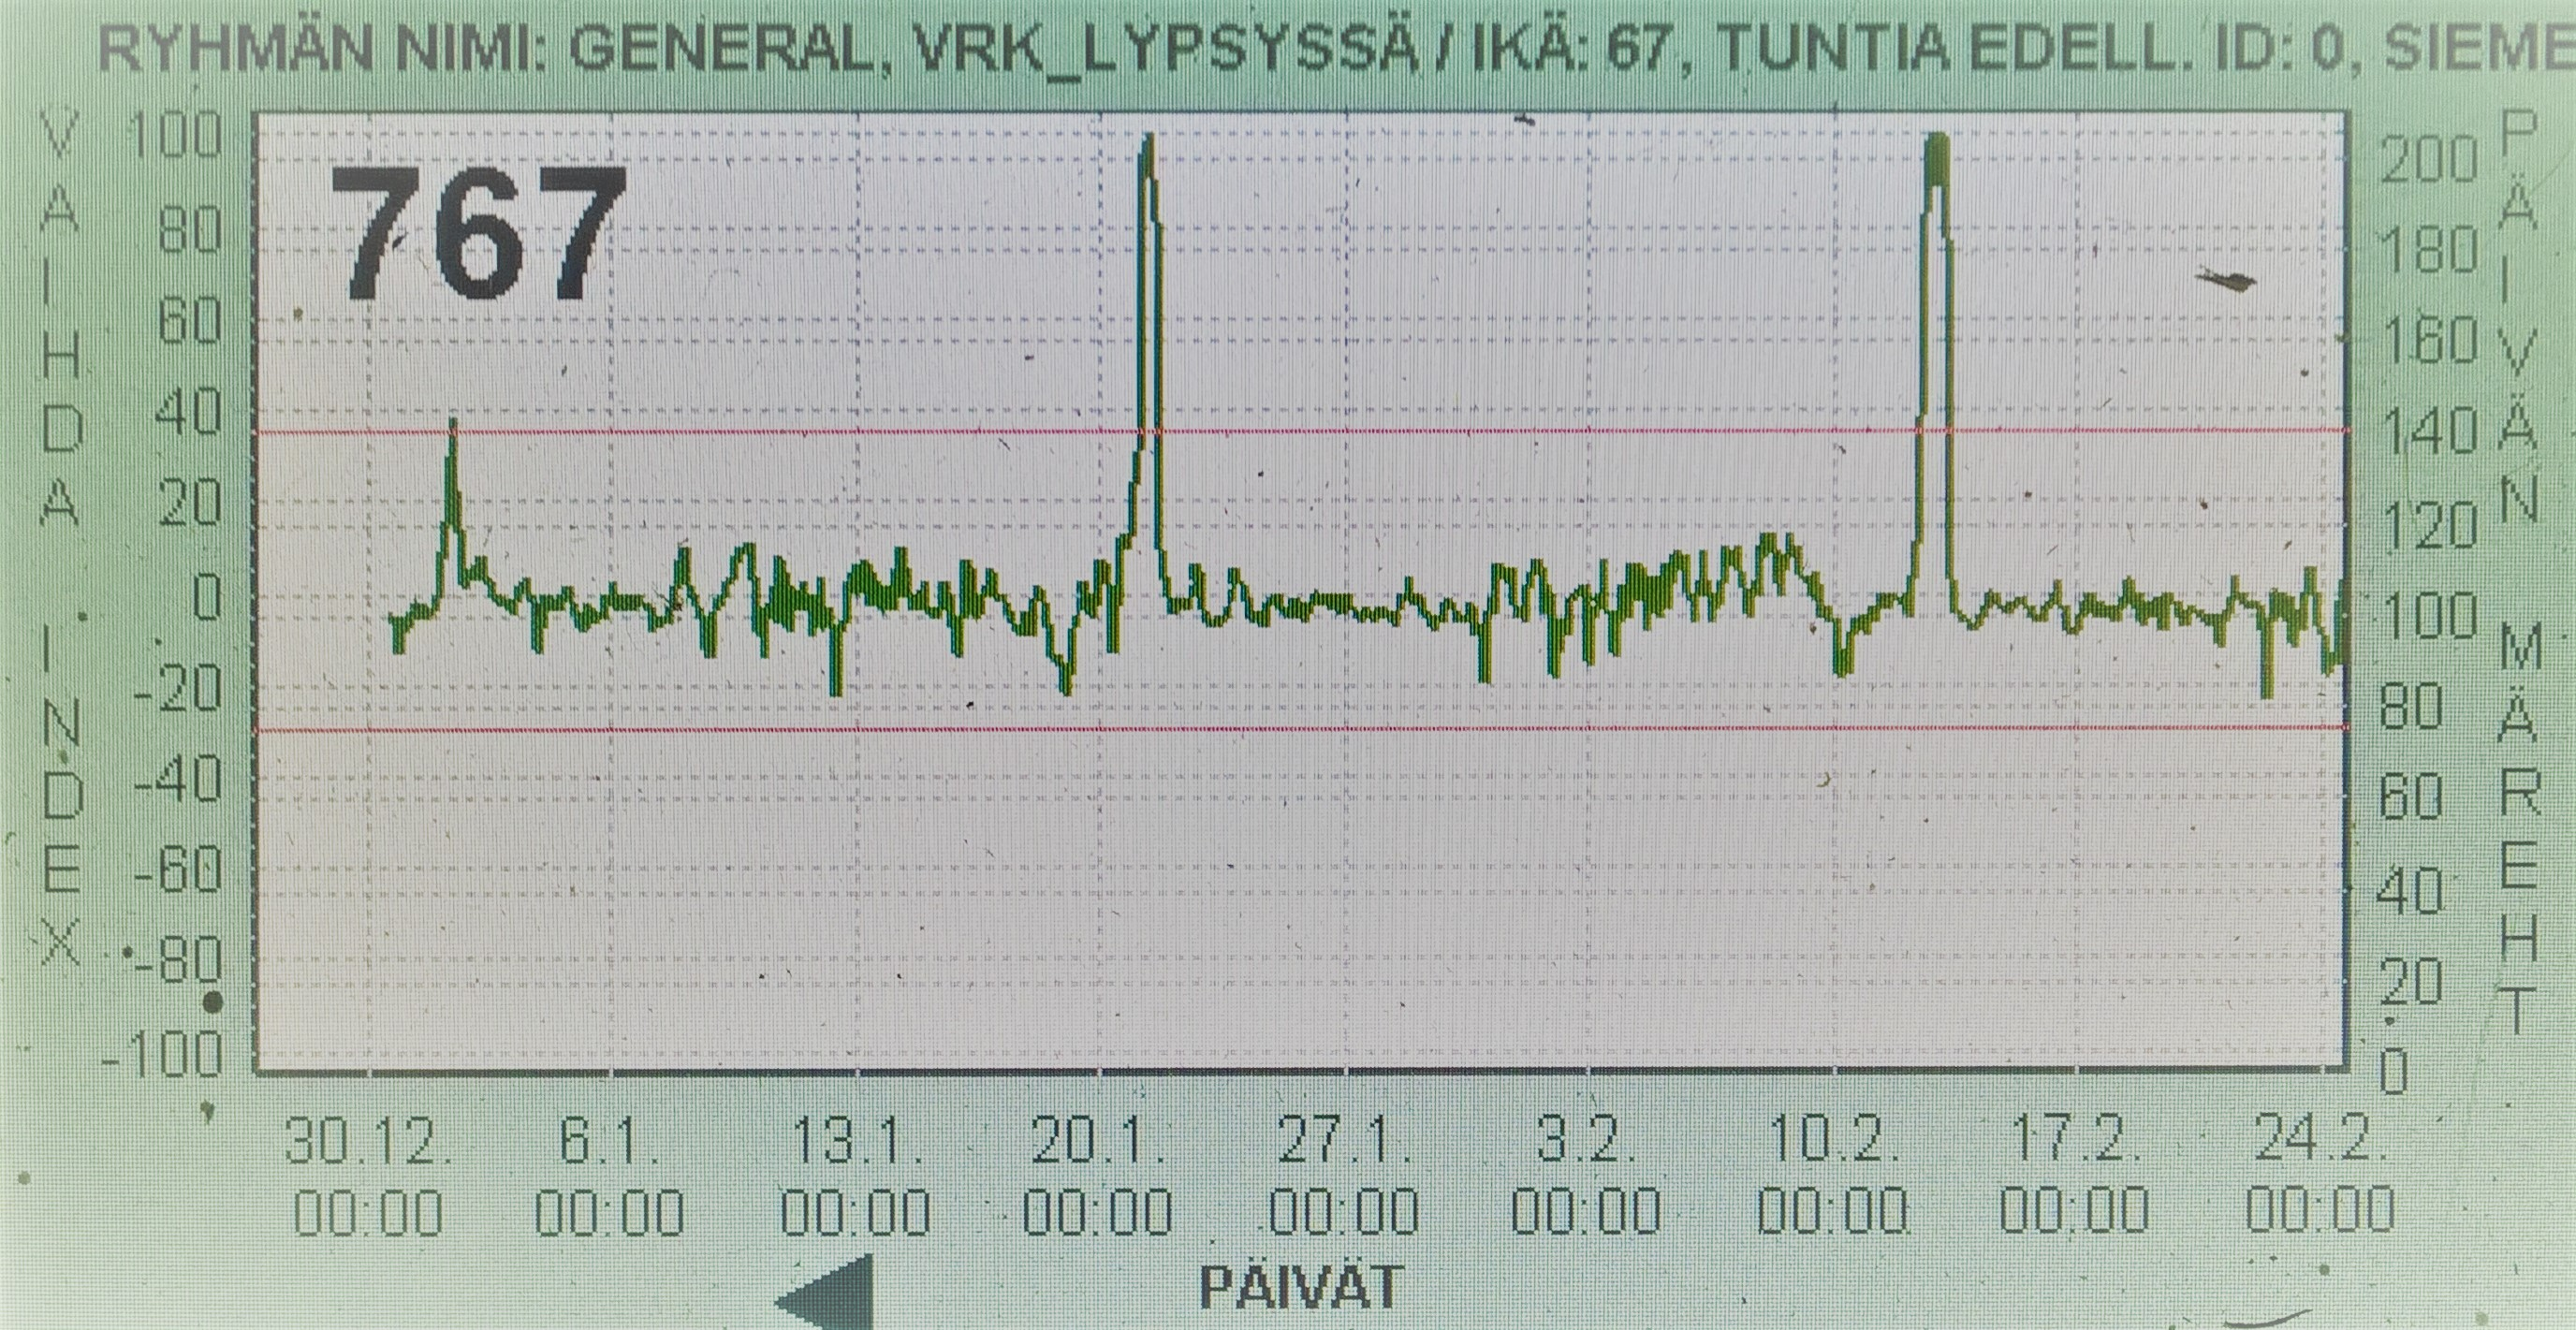
\includegraphics[width = 0.75\textwidth]{figures/heatime_kiima_767}
\caption{The activity data of Heatime system of the cow 767. The cow has had estruses approximately on January the 21\textsuperscript{st} and February the 13\textsuperscript{th}. The latter of the estruses should be detectable in this study, hence it is within our data recording period.}
\label{heatime_kiima_767_2}
\end{figure}

\begin{figure}[h]
\centering
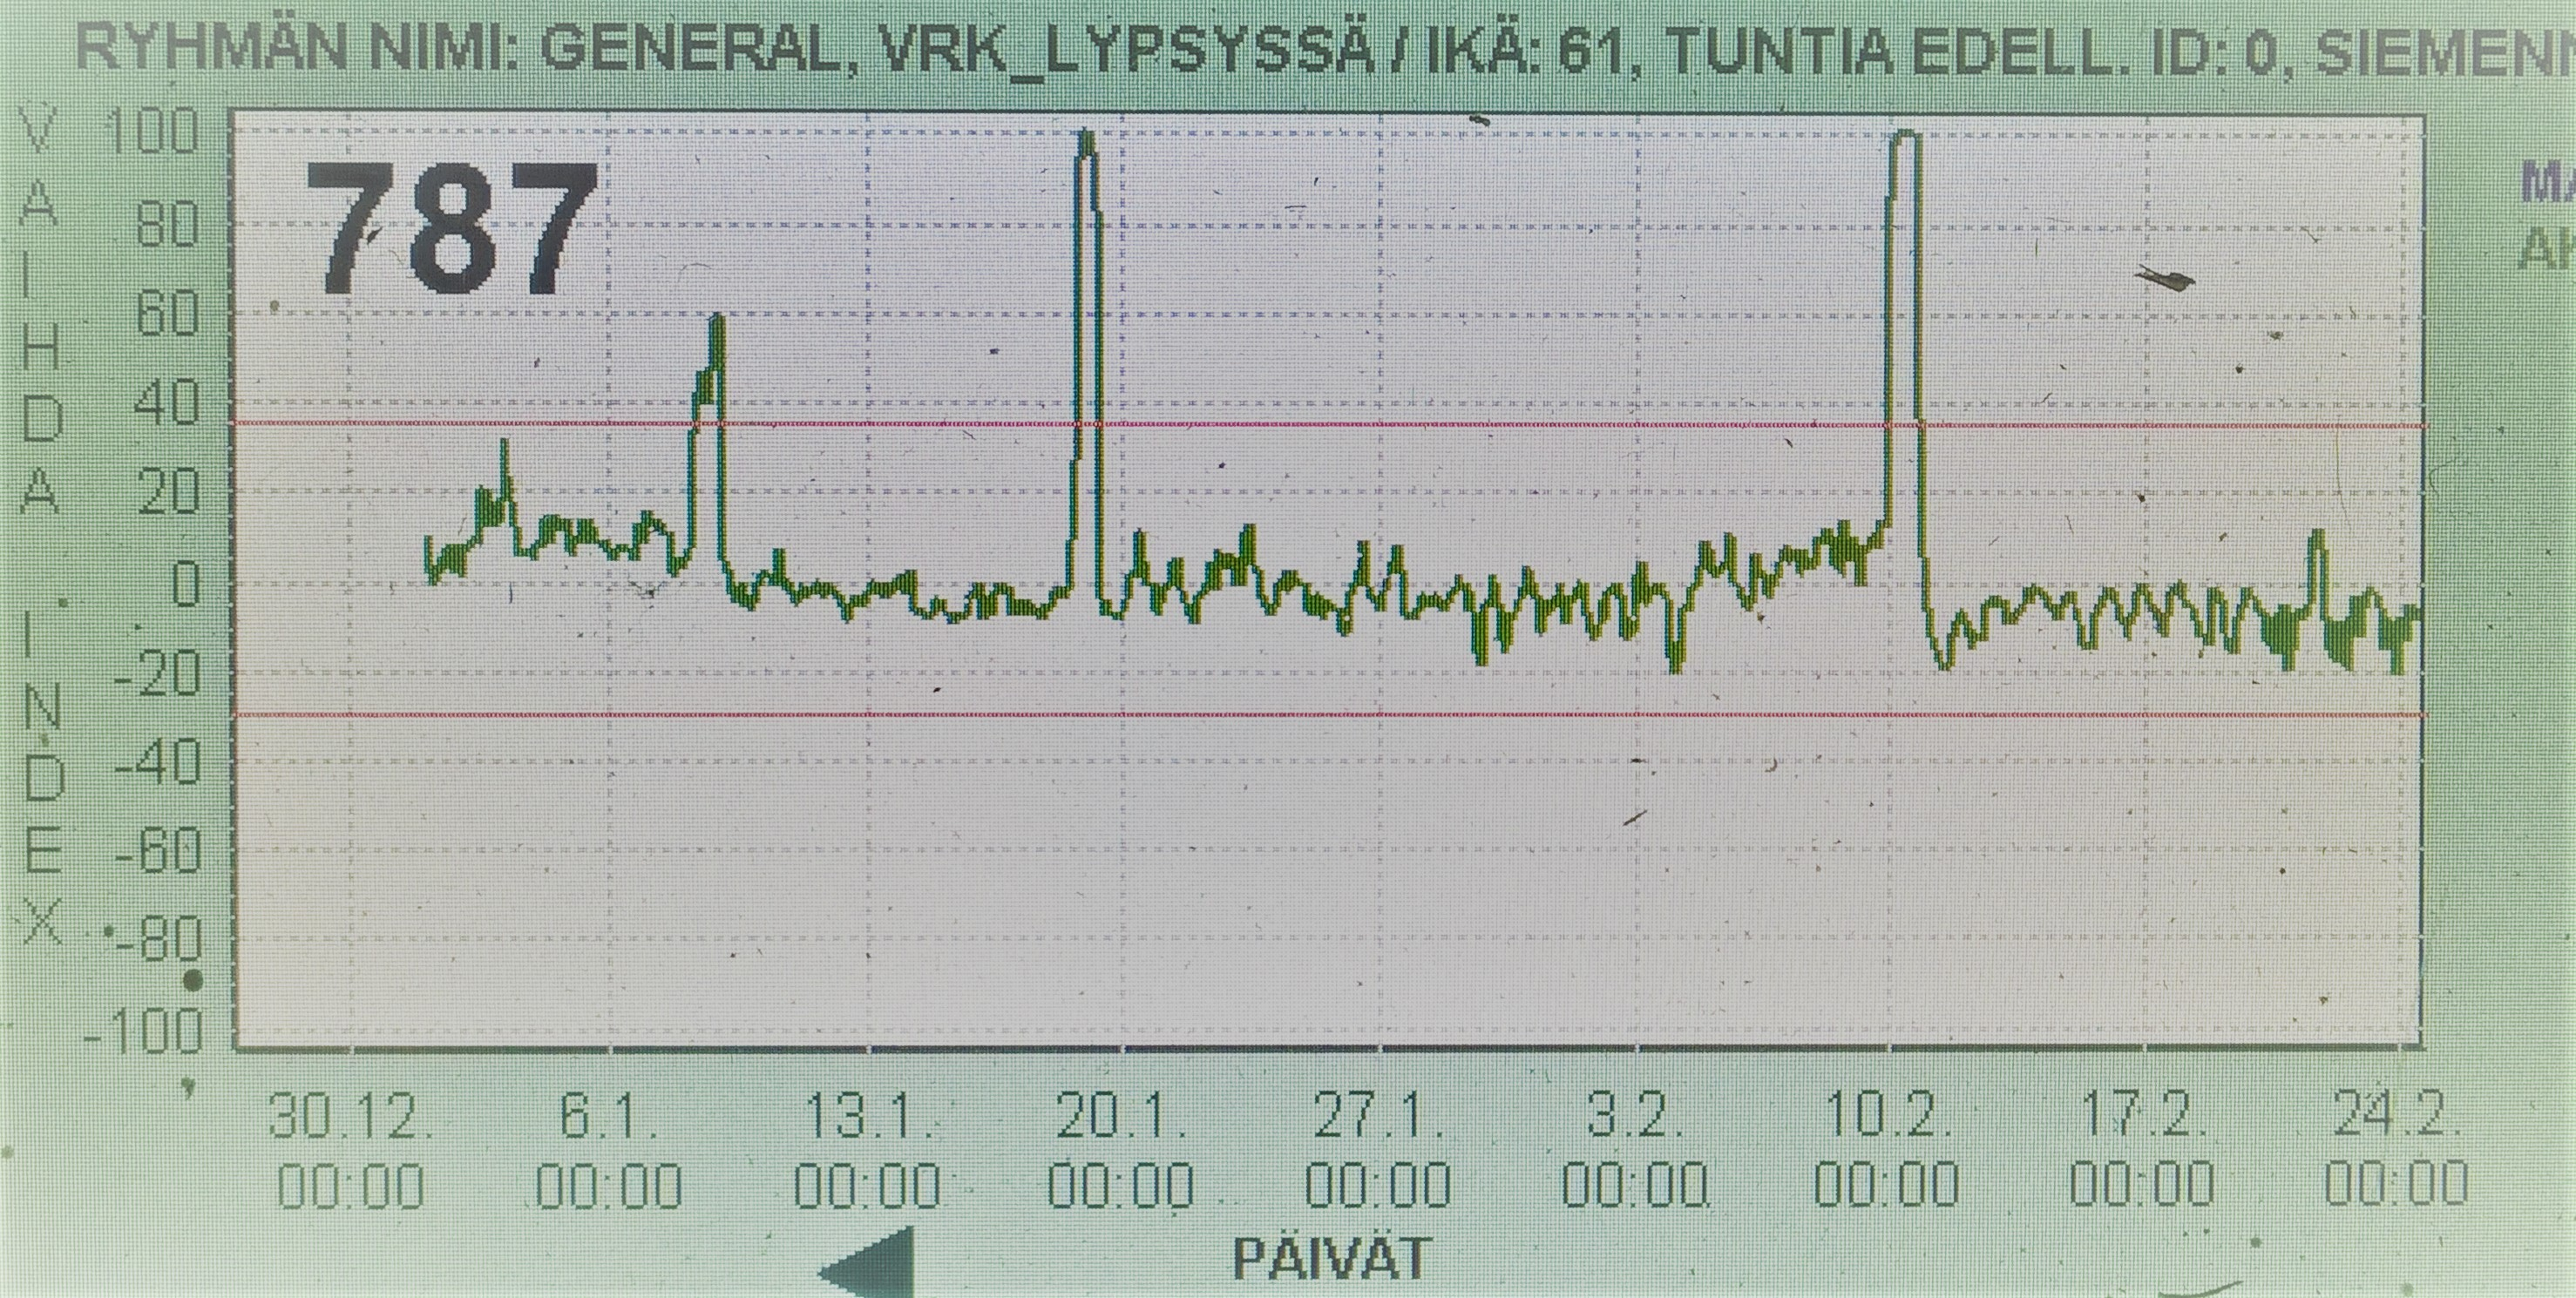
\includegraphics[width = 0.75\textwidth]{figures/heatime_kiima_787}
\caption{The activity data of Heatime system of the cow 787. The cow has had estruses approximately on January the 19\textsuperscript{th} and February the 10\textsuperscript{th}. The latter of the estruses should detectable in this study, hence it is within our data recording period.}
\label{heatime_kiima_787}
\end{figure}



\clearpage
\section{Raw Accelerometric Data}

\begin{figure}[h]
\centering
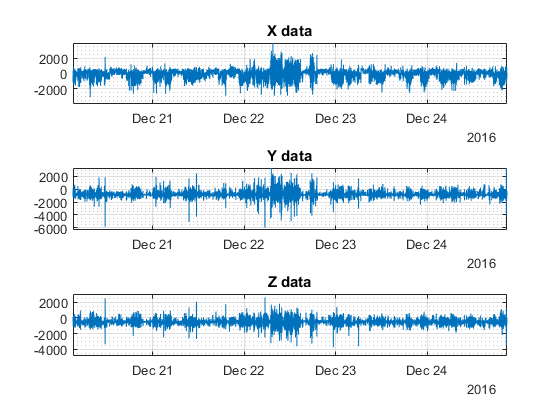
\includegraphics[width = 0.75\textwidth]{figures/kiimadata_9885_1.png}
\caption{The raw acceleration data of each axis of the cow 9885. The time frame is scaled around the first detectable estrus period. }
\label{kiimadata_9885_1}
\end{figure}

\begin{figure}[h]
\centering
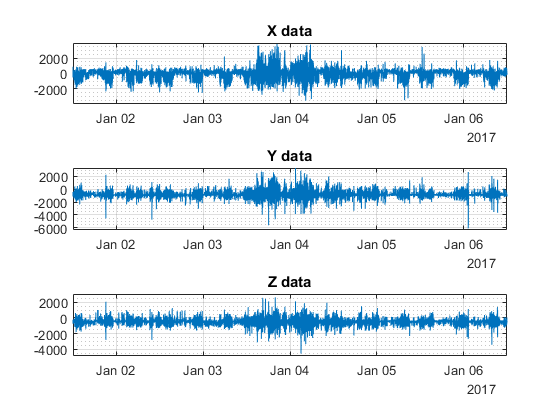
\includegraphics[width = 0.75\textwidth]{figures/kiimadata_9885_2.png}
\caption{The raw acceleration data of each axis of the cow 9885. The time frame is scaled around the second detectable estrus period. }
\label{kiimadata_9885_2}
\end{figure}

\clearpage
\section{Activity Monitoring Full Results}

\begin{figure}[h]
\centering
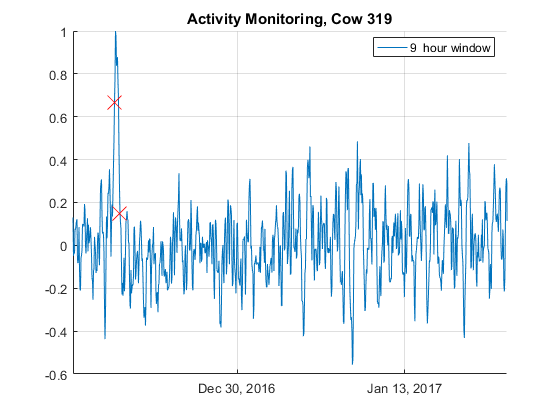
\includegraphics[width = 0.75 \textwidth]{figures/ActivityMonitoringCow319.png}
\caption{The plot of the results of the activity measurement algorithm of cow 319. A true positive estrus is detected and no false positive or false negative detection occurred. However, there is a lot of variation when not in estrus. Thus, the risk of false positive and false negative results is plausible.}
\label{ActivityMonitoringCow319}
\end{figure}

\begin{figure}[h]
\centering
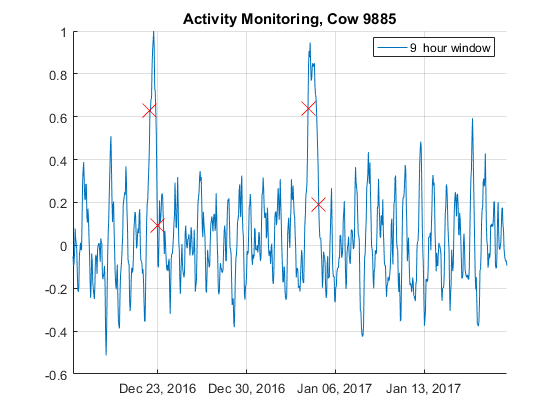
\includegraphics[width = 0.75 \textwidth]{figures/ActivityMonitoringCow9885.png}
\caption{The results of activity measurement of the cow 9885. Both of the estruses are detected. However, the difference between the estruses and the rest of the period is insignificant as it was with cow 319. Thus, the possibility of false positive and false negative results exists.}
\label{ActivityMonitoringCow9885}
\end{figure}

\begin{figure}[h]
\centering
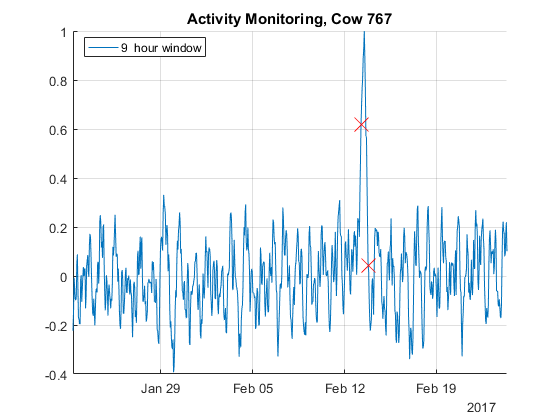
\includegraphics[width = 0.75 \textwidth]{figures/ActivityMonitoringCow767.png}
\caption{The plot of the activity measurement results of the cow 767. A true positive estrus is detected and no occurrence of false positives of false negatives. Additionally, the difference between proestrus and rest of the period is obvious. The risk of false positive or false negative results is minor. }
\label{ActivityMonitoringCow767}
\end{figure}

\begin{figure}[h]
\centering
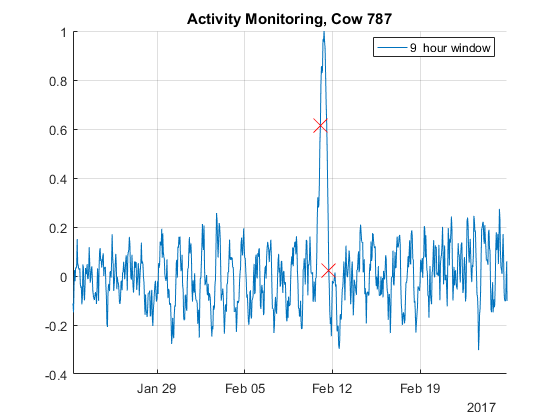
\includegraphics[width = 0.75 \textwidth]{figures/ActivityMonitoringCow787.png}
\caption{The results of activity measurement of the cow 787. The difference between the estrus and rest of the period is most distinct within this algorithm. Thus, the risk of false positive and false negative results is least significant.}
\label{ActivityMonitoringCow787}
\end{figure}

\begin{figure}[h]
\centering
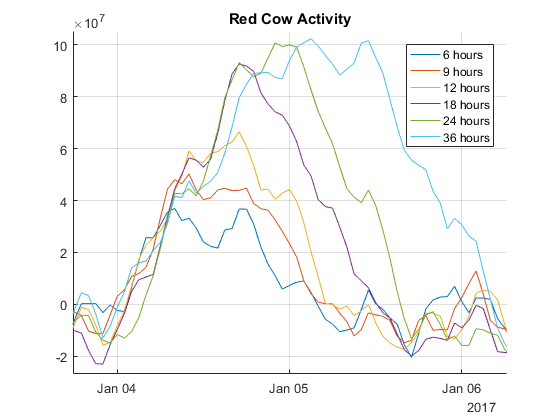
\includegraphics[width = 0.75\textwidth]{figures/redcowactivity2.png}
\caption{The activity plots of the second proestrus of the cow 9885. The figure illustrates the affect of varying the size of the integration window. Wider window increases the amplitude of the estrus and eases the detectability. However, simultaneously it delays the moment of detection. }
\label{integrationwindows}
\end{figure}

\clearpage
\section{Variance Detection Full Results}

\begin{figure}[h]
\centering
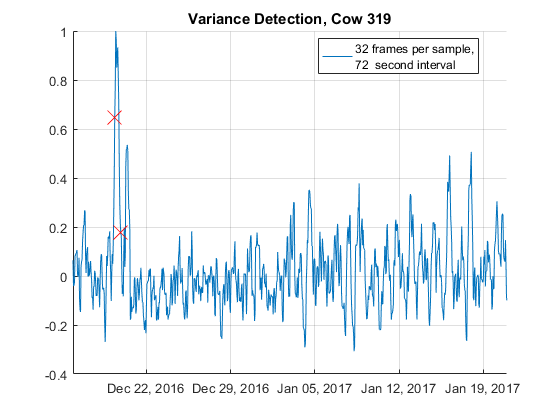
\includegraphics[width = 0.75 \textwidth]{figures/VarianceDetectionCow319.png}
\caption{The results of the variance detection algorithm of the cow 319. The estrus on December the 20\textsuperscript{th} is barely detectable. Additionally, algorithm yielded several false positive estruses. Furthermore, the amplitude of the false positives exceeds the true positive.}
\label{VarianceDetectionCow319}
\end{figure}

\begin{figure}[h]
\centering
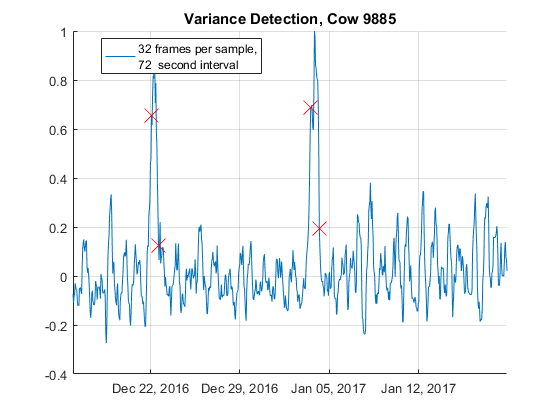
\includegraphics[width = 0.75 \textwidth]{figures/VarianceDetectionCow9885.png}
\caption{The results of variance detection algorithm of the cow 9885. The true positive estrus is detected on December the 22\textsuperscript{st}. Furthermore, the amplitude difference between the detected estrus and other period is significant. However, the algorithm yield a false negative on January the 4\textsuperscript{th}.}
\label{VarianceDetectionCow9885}
\end{figure}

\begin{figure}[h]
\centering
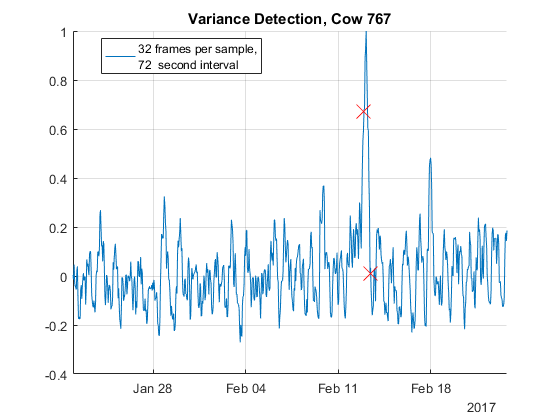
\includegraphics[width = 0.75 \textwidth]{figures/VarianceDetectionCow767.png}
\caption{The variance detection results of the cow 767. There are multiple false positive detections in the data period. In general, there is no obvious difference between the estrus and non-estrus periods. Nevertheless, a true positive estrus is detected on February the 13\textsuperscript{th}.}
\label{VarianceDetectionCow767}
\end{figure}

\begin{figure}[h]
\centering
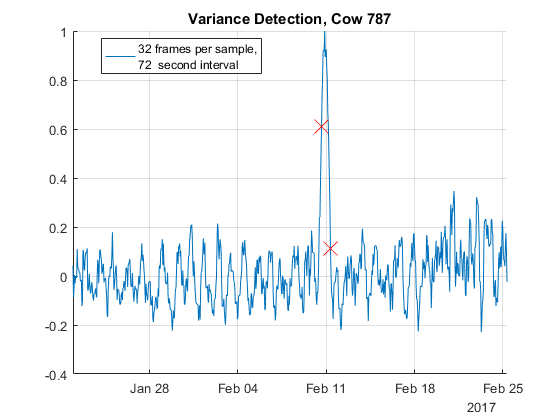
\includegraphics[width = 0.75 \textwidth]{figures/VarianceDetectionCow787.png}
\caption{The results of variance detection algorithm of the cow 787. The true positive estrus is detected on February the 10\textsuperscript{th}. However, a false positive detection occurred on February the 21\textsuperscript{st}. Otherwise, the amplitude  difference between estrus and non-estrus periods is obvious.}
\label{VarianceDetectionCow787}
\end{figure}

\begin{figure}[h]
\centering
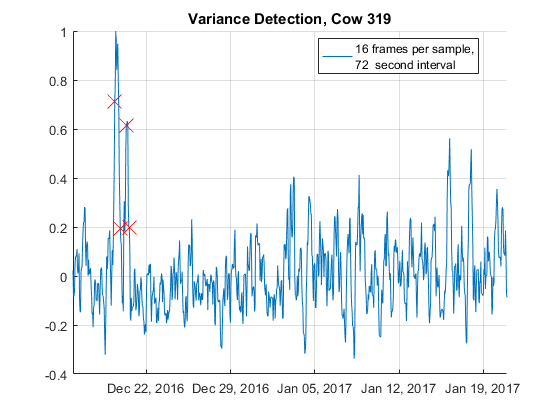
\includegraphics[width = 0.75 \textwidth]{figures/VarianceDetectionCow319_16frames72seconds.png}
\caption{Reducing the sample size to 16 frames per sample and keeping the sampling interval in 72 seconds yields false positive results with the cow 319}
\label{}
\end{figure}

\begin{figure}[h]
\centering
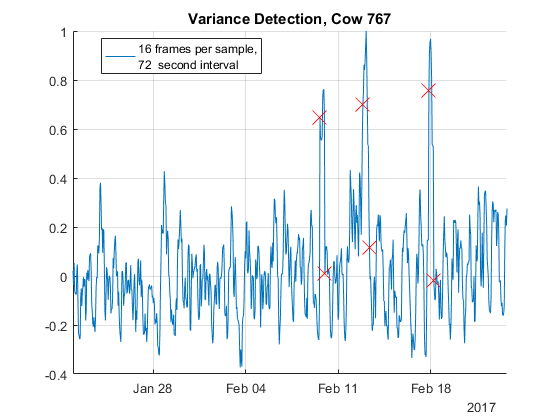
\includegraphics[width = 0.75 \textwidth]{figures/VarianceDetectionCow767_16frames72seconds.png}
\caption{Reducing the sample size to 16 frames per sample and keeping the sampling interval in 72 seconds yields false positive results with the cow 767}
\label{}
\end{figure}

%------------%

\begin{figure}[h]
\centering
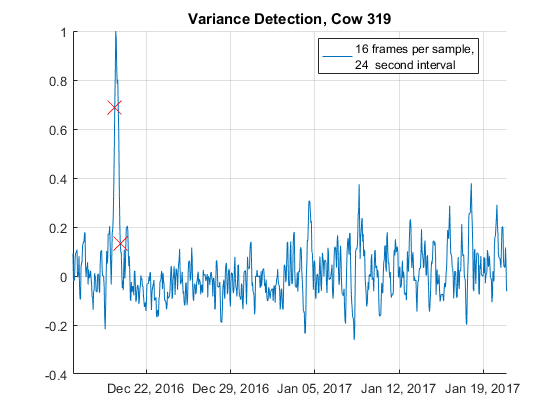
\includegraphics[width = 0.75 \textwidth]{figures/VarianceDetectionCow319_16frames24seconds.png}
\caption{Reducing the sample size to 16 frames and increasing the sampling interval to 24 seconds improves the performance of the variance detection algorithm. Consequently, no false positive results occurs.}
\label{}
\end{figure}

\begin{figure}[h]
\centering
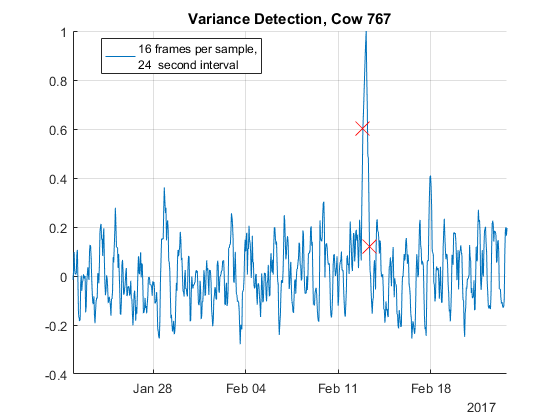
\includegraphics[width = 0.75 \textwidth]{figures/VarianceDetectionCow767_16frames24seconds.png}
\caption{Reducing the sample size to 16 frames and increasing the sampling interval to 24 seconds improves the performance of the variance detection algorithm. Consequently, no false positive results occurs.}
\label{}
\end{figure}


Varying the sampling interval affect the results:


\begin{figure}[h]
\centering
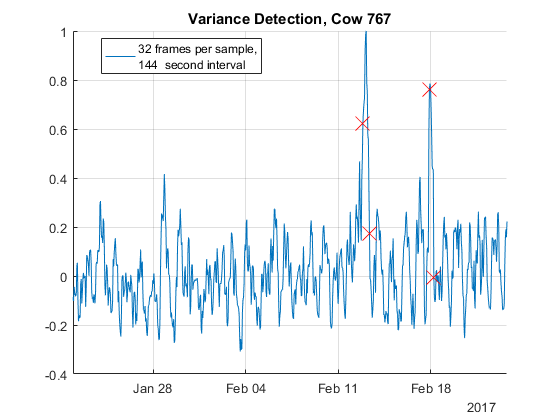
\includegraphics[width = 0.75 \textwidth]{figures/VarianceDetectionCow767_32frames144seconds.png}
\caption{More seldom sampling yield false positive results as seen in this picture.}
\label{}
\end{figure}


\begin{figure}[h]
\centering
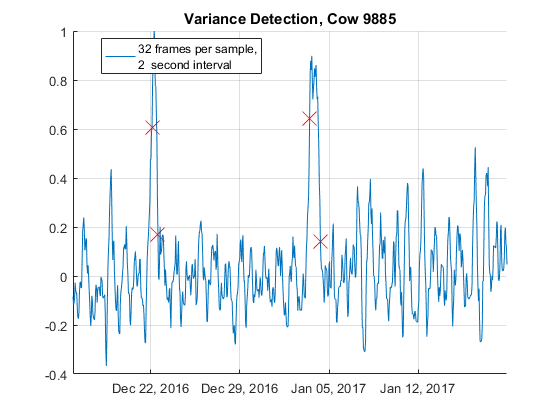
\includegraphics[width = 0.75 \textwidth]{figures/VarianceDetectionCow9885_32frames2seconds.png}
\caption{Decreasing the sampling interval does not directly improve the results as it is with the cow 9885. This sampling frequency corresponds approximately continuous sampling. Nevertheless, the results are worse than formerly.}
\label{}
\end{figure}



\begin{figure}[h]
\centering
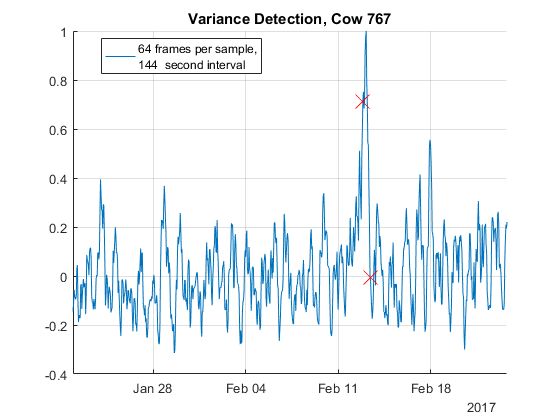
\includegraphics[width = 0.75 \textwidth]{figures/VarianceDetectionCow767_64frames144seconds.png}
\caption{}
\label{}
\end{figure}

\begin{figure}[htb]
\centering
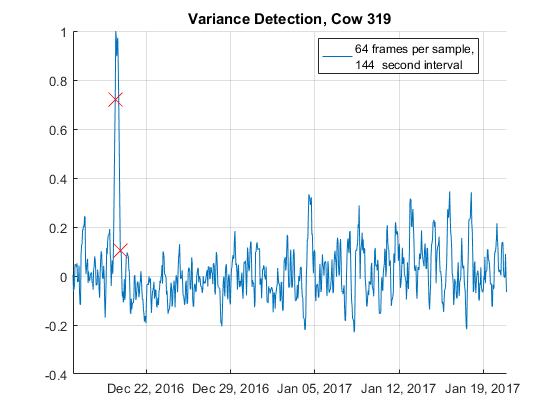
\includegraphics[width = 0.75 \textwidth]{figures/VarianceDetectionCow319_64frames144seconds.png}
\caption{}
\label{}
\end{figure}

\begin{figure}[h]
\centering
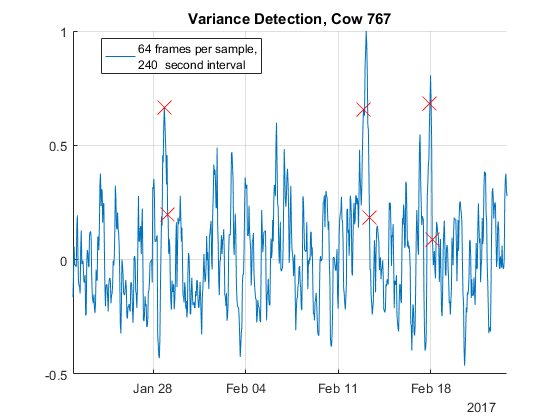
\includegraphics[width = 0.75 \textwidth]{figures/VarianceDetectionCow767_64frames240seconds.png}
\caption{}
\label{}
\end{figure}


\clearpage
\section{Inactivity Detection Full Results}


\begin{figure}[h]
\centering
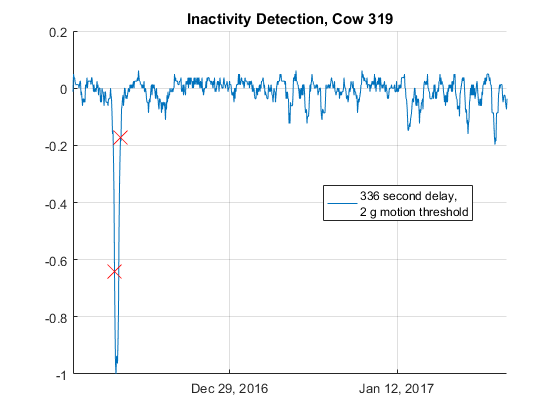
\includegraphics[width = 0.75 \textwidth]{figures/InactivityDetectionCow319.png}
\caption{The results of the inactivity detection algorithm of the cow 319. The parameters are 336 second delay and \SI{2}{\gram} motion threshold. A true positive estrus is detected on December the 20\textsuperscript{th}. The amplitude of proestrus and non-estrus is significant. }
\label{InactivityDetectionCow319}
\end{figure}


\begin{figure}[h]
\centering
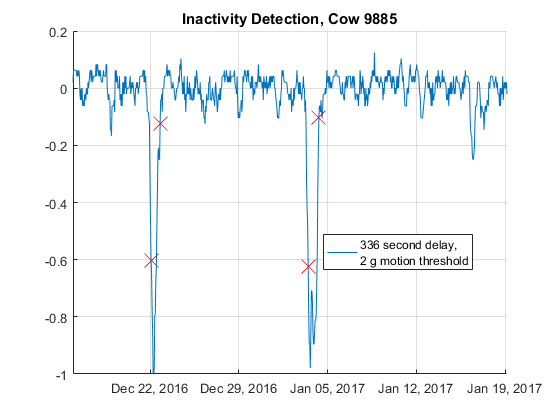
\includegraphics[width = 0.75 \textwidth]{figures/InactivityDetectionCow9885.png}
\caption{The results of inactivity detection algorithm of the cow 9885. The parameters are 336 second delay and \SI{2}{\gram} motion threshold. Both of the estruses are detected as true positive on December the 22\textsuperscript{nd} and January the 4\textsuperscript{th}. No false positive or false negative detection occurred. The amplitude difference between proestrus and non-estrus is obvious.}
\label{InactivityDetectionCow9885}
\end{figure}


\begin{figure}[h]
\centering
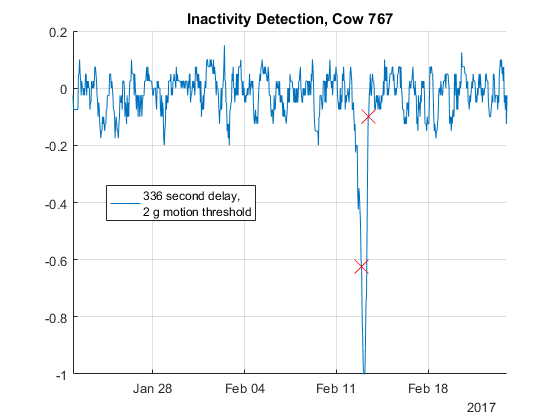
\includegraphics[width = 0.75 \textwidth]{figures/InactivityDetectionCow767.png}
\caption{The results of the inactivity detection algorithm of the cow 767. The parameters are 336 second delay and \SI{2}{\gram} motion threshold. A true positive estrus is detected on February the 13\textsuperscript{th}. Additionally, the amplitude of the proestrus differs from none-estrus significantly.}
\label{InactivityDetectionCow767}
\end{figure}

\begin{figure}[h]
\centering
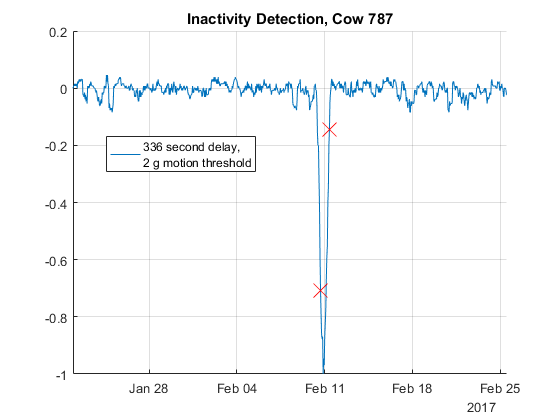
\includegraphics[width = 0.75 \textwidth]{figures/InactivityDetectionCow787.png}
\caption{The results of inactivity detection algorithm of the cow 787. The parameters are 336 second delay and \SI{2}{\gram} motion threshold. A ture positive estrus is detected on February the 11\textsuperscript{th} and no false positives of false negatives occurred. Furthermore, the difference between estrus and other periods is most significant.}
\label{InactivityDetectionCow787}
\end{figure}



\begin{figure}[h]
\centering
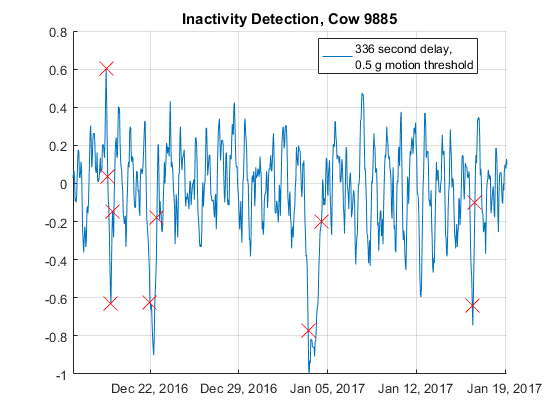
\includegraphics[width = 0.75 \textwidth]{figures/InactivityDetectionCow9885_336period05threshold.png}
\caption{}
\label{}
\end{figure}

\begin{figure}[h]
\centering
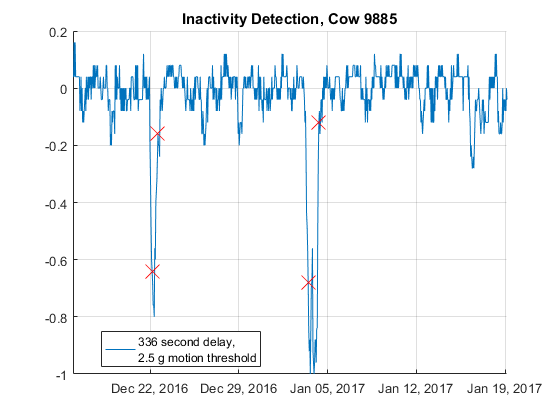
\includegraphics[width = 0.75 \textwidth]{figures/InactivityDetectionCow9885_336period2_5threshold.png}
\caption{}
\label{}
\end{figure}

\begin{figure}[h]
\centering
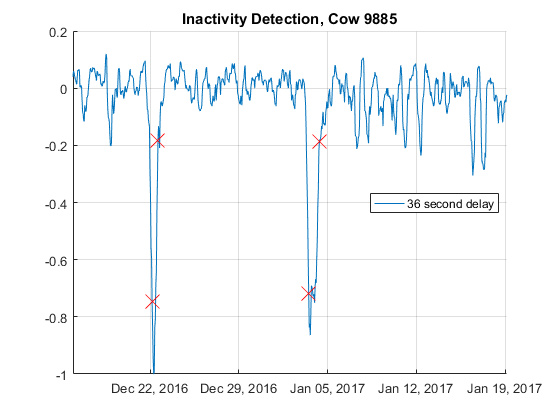
\includegraphics[width = 0.75 \textwidth]{figures/InactivityDetectionCow9885_36period.png}
\caption{}
\label{}
\end{figure}

\begin{figure}[h]
\centering
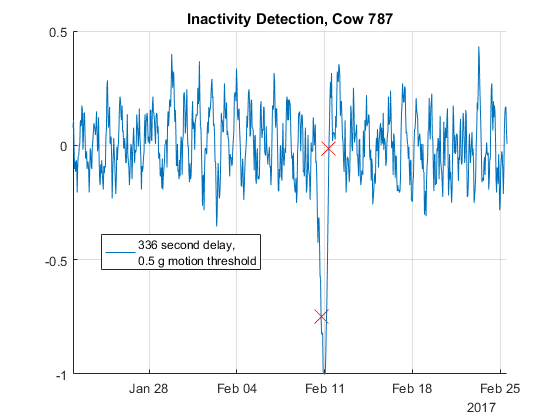
\includegraphics[width = 0.75 \textwidth]{figures/InactivityDetectionCow787_336period05threshold.png}
\caption{}
\label{}
\end{figure}

\begin{figure}[h]
\centering
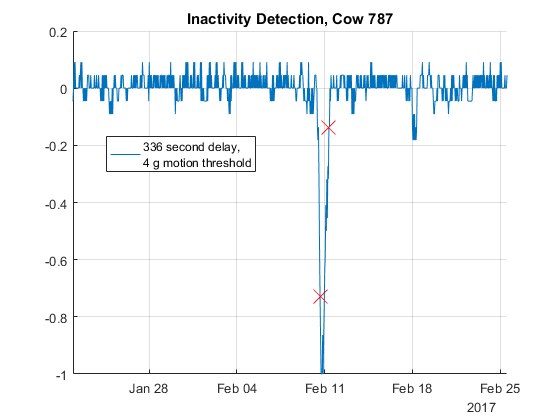
\includegraphics[width = 0.75 \textwidth]{figures/InactivityDetectionCow787_336period4threshold.png}
\caption{}
\label{}
\end{figure}

\begin{figure}[h]
\centering
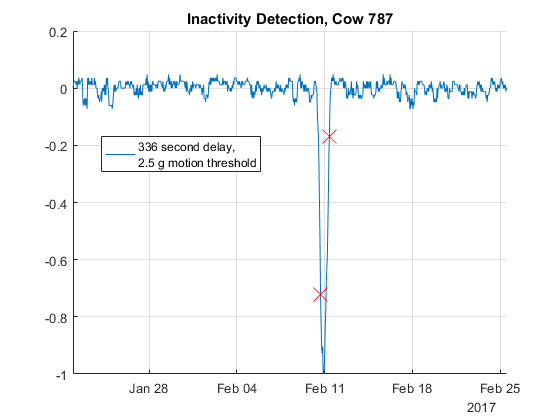
\includegraphics[width = 0.75 \textwidth]{figures/InactivityDetectionCow787_336period2_5threshold.png}
\caption{}
\label{}
\end{figure}

\begin{figure}[h]
\centering
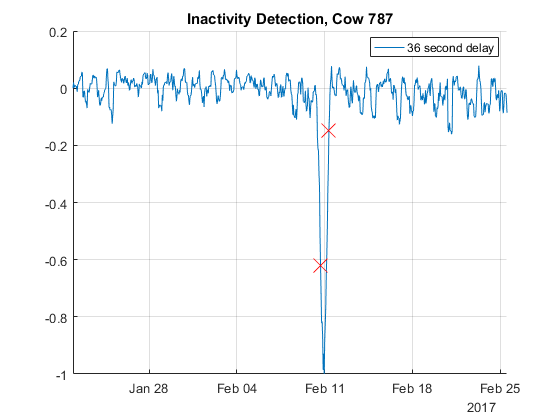
\includegraphics[width = 0.75 \textwidth]{figures/InactivityDetectionCow787_36period.png}
\caption{}
\label{}
\end{figure}

\begin{figure}[h]
\centering
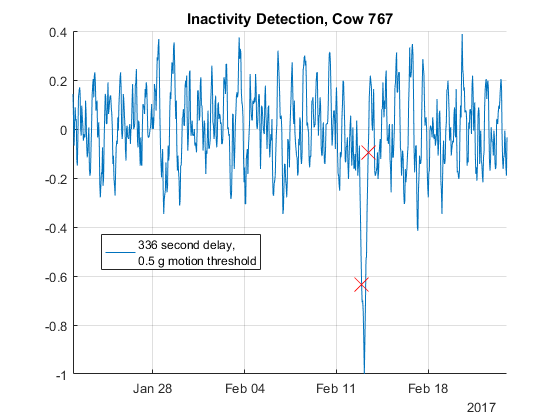
\includegraphics[width = 0.75 \textwidth]{figures/InactivityDetectionCow767_336period05threshold.png}
\caption{}
\label{}
\end{figure}

\begin{figure}[h]
\centering
\includegraphics[width = 0.75 \textwidth]{figures/InactivityDetectionCow767_336period4threshold.png}
\caption{}
\label{}
\end{figure}


\begin{figure}[h]
\centering
\includegraphics[width = 0.75 \textwidth]{figures/InactivityDetectionCow767_336period2_5threshold.png}
\caption{}
\label{}
\end{figure}

\begin{figure}[h]
\centering
\includegraphics[width = 0.75 \textwidth]{figures/InactivityDetectionCow767_36period.png}
\caption{}
\label{}
\end{figure}

\begin{figure}[h]
\centering
\includegraphics[width = 0.75 \textwidth]{figures/InactivityDetectionCow319_336period05threshold.png}
\caption{}
\label{}
\end{figure}

\begin{figure}[h]
\centering
\includegraphics[width = 0.75 \textwidth]{figures/InactivityDetectionCow319_336period2_5threshold.png}
\caption{}
\label{}
\end{figure}

\begin{figure}[h]
\centering
\includegraphics[width = 0.75 \textwidth]{figures/InactivityDetectionCow319_36period.png}
\caption{}
\label{}
\end{figure}




%
%\section{Esimerkki liitteestä\label{LiiteA}}
%
%Liitteet eivät ole opinnäytteen kannalta välttämättömiä ja 
%opinnäytteen tekijän on 
%kirjoittamaan ryhtyessään hyvä ajatella pärjäävänsä ilman liitteitä.
%Kokemattomat kirjoittajat, jotka ovat huolissaan
%tekstiosan pituudesta, paisuttavat turhan 
%helposti liitteitä pitääkseen tekstiosan pituuden annetuissa rajoissa.
%Tällä tavalla ei synny hyvää opinnäytettä.   
%
%Liite on itsenäinen kokonaisuus, vaikka se täydentääkin tekstiosaa.
%Liite ei siten ole pelkkä listaus, kuva tai taulukko, vaan 
%liitteessä selitetään aina sisällön laatu ja tarkoitus. 
%
%Liitteeseen voi laittaa esimerkiksi listauksia. Alla on 
%listausesimerkki tämän liitteen luomisesta. 
%
%%% Verbatim-ympäristö ei muotoile tai tavuta tekstiä. Fontti on monospace.
%%% Verbatim-ympäristön sisällä annettuja komentoja ei LaTeX käsittele. 
%%% Vasta \end{verbatim}-komennon jälkeen jatketaan käsittelyä.
%\begin{verbatim}
%	\clearpage
%	\appendix
%	\addcontentsline{toc}{section}{Liite A}
%	\section*{Liite A}
%	...
%	\thispagestyle{empty}
%	...
%	tekstiä
%	...
%	\clearpage
%\end{verbatim}
%
%Kaavojen numerointi muodostaa liitteissä oman kokonaisuutensa:
%\begin{eqnarray}
%d \wedge A  &=& F, \label{liitekaava1}\\
%d \wedge F  &=& 0. \label{liitekaava2}
%\end{eqnarray}
%
%
%\clearpage
%\section{Toinen esimerkki liitteestä\label{LiiteB}}
%
%%% Liitteiden kaavat, taulukot ja kuvat numeroidaan omana kokonaisuutenaan
%
%Liitteissä voi myös olla kuvia, jotka
%eivät sovi leipätekstin joukkoon:
%%% Ympäristön figure parametrit htb pakottavat
%%% kuvan tähän, eikä LaTeX yritä siirrellä niitä
%%% hyväksi katsomaansa paikkaan. 
%%% Ympäristöä center voi käyttää \centering-
%%% komennon sijaan
%%%
%\begin{figure}[htb]
%\begin{center}
%\includegraphics[height=8cm]{kuva2}
%\end{center}
%\caption{Kuvateksti, jossa on liitteen numerointi}
%\label{liitekuva}
%\end{figure}
%%%
%Liitteiden taulukoiden numerointi on kuvien ja kaavojen kaltainen:
%\begin{table}[htb]
%\caption{Taulukon kuvateksti.}
%\label{liitetaulukko}
%\begin{center}
%\fbox{
%\begin{tabular}{lp{0.5\linewidth}}
%9.00--9.55  & Käytettävyystestauksen tiedotustilaisuus (osanottajat
%ovat saaneet sähköpostitse valmistautumistehtävät, joten tiedotustilaisuus
%voidaan pitää lyhyenä).\\
%9.55--10.00 & Testausalueelle siirtyminen
%\end{tabular}}
%\end{center}
%\end{table}
%Kaavojen numerointi muodostaa liitteissä oman kokonaisuutensa:
%\begin{eqnarray}
%T_{ik} &=& -p g_{ik} + w u_i u_k + \tau_{ik},  \label{liitekaava3} \\
%n_i    &=& n u_i + v_i.                      \label{liitekaava4}
%\end{eqnarray}


\end{document}
